
\documentclass[12pt,twoside]{reedthesis}

\usepackage{graphicx,latexsym} 
\usepackage{amssymb,amsthm,amsmath}
\usepackage{longtable,booktabs,setspace}
\usepackage[hyphens]{url}
\usepackage{rotating}
\usepackage{natbib}
%\usepackage{xcolor}
\usepackage[dvipsnames]{xcolor}
\usepackage{scrextend}
\usepackage{caption}
\usepackage{subcaption}
\usepackage{float}

% pdflatex --shell-escape svg.tex;

\newcommand{\code}[1]{\texttt{#1}}
% Comment out the natbib line above and uncomment the following two lines to use the new 
% biblatex-chicago style, for Chicago A. Also make some changes at the end where the 
% bibliography is included. 
%\usepackage{biblatex-chicago}
%\bibliography{thesis}

% \usepackage{times} % other fonts are available like times, bookman, charter, palatino

\title{The L-Systems Explorer: An Introduction to Generative Art} % Not really an introduction. There's probably a better way to describe this
\author{R Jacob Hoopes}
\date{May 2023}
\division{Mathematics and Natural Sciences}
\advisor{Dylan McNamee}
\department{Computer Science}

\setlength{\parskip}{0pt}
%%
%% End Preamble
%%
%% The fun begins:
\begin{document}

  \maketitle
  \frontmatter % this stuff will be roman-numbered
  \pagestyle{empty} % this removes page numbers from the frontmatter

% Acknowledgements (Acceptable American spelling) are optional
% So are Acknowledgments (proper English spelling)
    \chapter*{Acknowledgements}
	This thesis has been a joy to put together. I've reveled in each opportunity to engage with the material and explore more about this idea whose depth I feel I have only begun to understand. Engaging with my peers and mentors about L-Systems and Generative Art has opened my mind to new ways of thinking about these ideas, not to mention the joy I feel when they respond with their interests in kind. I've attempted to make this thesis multidisciplinary, in the spirit of L-Systems as a child of both Art and Computer Science, but also in the spirit of Reed College as a Liberal Arts institution. For this, and in all things, I have found that no idea is complete without a range of perspectives.
	
	I'm grateful to Sky Peterson, Jon DeVries, Jaden Nichols, Aria Killebrew Bruehl, Izzy McKenna, Keith Ng, Will Howes, Astrid Lilly, Nathan Hagan, Izzy Laun, Ariana Fleet, Calvin Beeman-Weber, Ross Tidwell, Miles Silvey, and all the others who I've talked with about the construction of this thesis. You've kept me afloat.
	
	Unending thanks to my roommates, Henry Wilson, Brent Ellis, and Gabe Fish for your support in everything. This would not be possible at all without your presence. With Bridge, Root, and whatever other new thing we have going on, this has only happened because I've been able to retreat back to a loving home when I'm done with my work. My gratitude really surpasses expression.
	
	
	%\textit{The cell has been the ``tangible immaterial means of representation for everything. [...] [these things are] realities that emerge from handwork,"} - Rainer Maria Rilke, - Kelty and Landecker (58)
	
	%\textcolor{blue}{[A large, beautiful L-System]}
	
	%\includesvg{pretty}
	\begin{figure}[h]
	\centering
	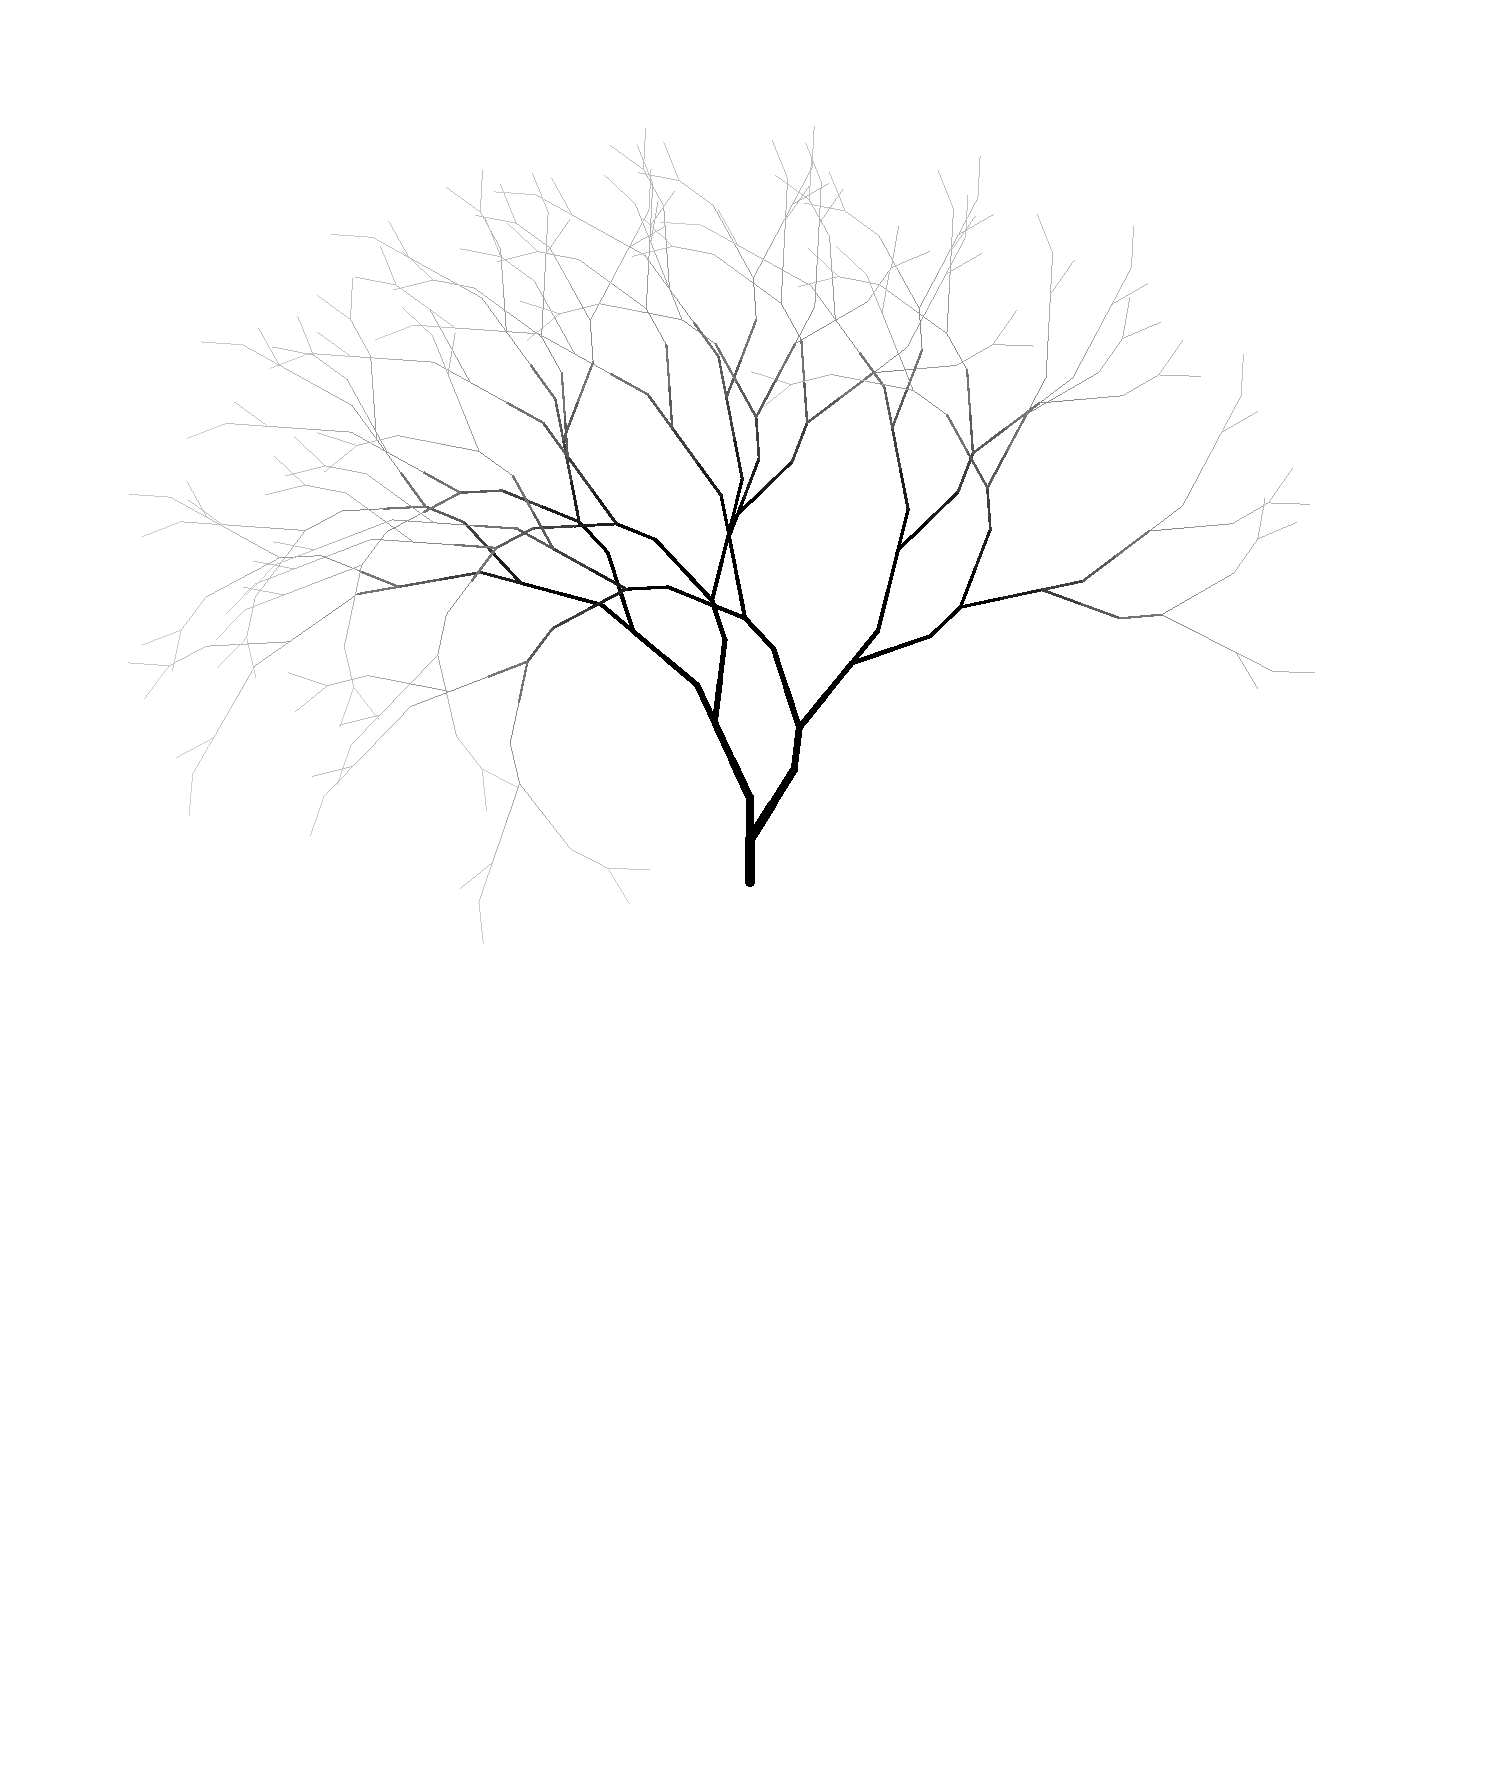
\includegraphics[clip=true, viewport=1in 5.5in 9in 11.3in, scale=0.49]{Images/Acknowledgements1}
	\caption[Gratitude]{Gratitude\footnotemark}
	\label {Acknowledgements1}
	\end{figure}
	\footnotetext{A; A $\rightarrow$ F[F+FA]-FB, B $\rightarrow$ F+F[–FA]+FB; $\theta$ = 32$^{\circ}$, $\phi$ = -7$^{\circ}$; Iterations = 7; IW = 4.5, WC = 0.85}
	


    \tableofcontents
% if you want a list of tables, optional
   % \listoftables
% if you want a list of figures, also optional
	\listoffigures

% The abstract is not required if you're writing a creative thesis (but aren't they all?)
% If your abstract is longer than a page, there may be a formatting issue.
\chapter*{Abstract}
	The world is a mess of systems. I hope to establish the context for one system that interests me and build it up for you so that you may be as interested in it as I have been. There will be an overview of the structure and function of L-Systems, later followed by the brief introduction of some different types of L-Systems. I'll explain the program that allows users to learn about and explore L-Systems, followed by a demonstration of its capabilities and its development. I will also discuss some related work, and go on to explain possible extensions. Wrapping things up, I take a step back from the program to ask some larger questions.
	
	%\textcolor{blue}{[Another large, beautiful L-System]}
	\begin{figure}[h]
	\centering
	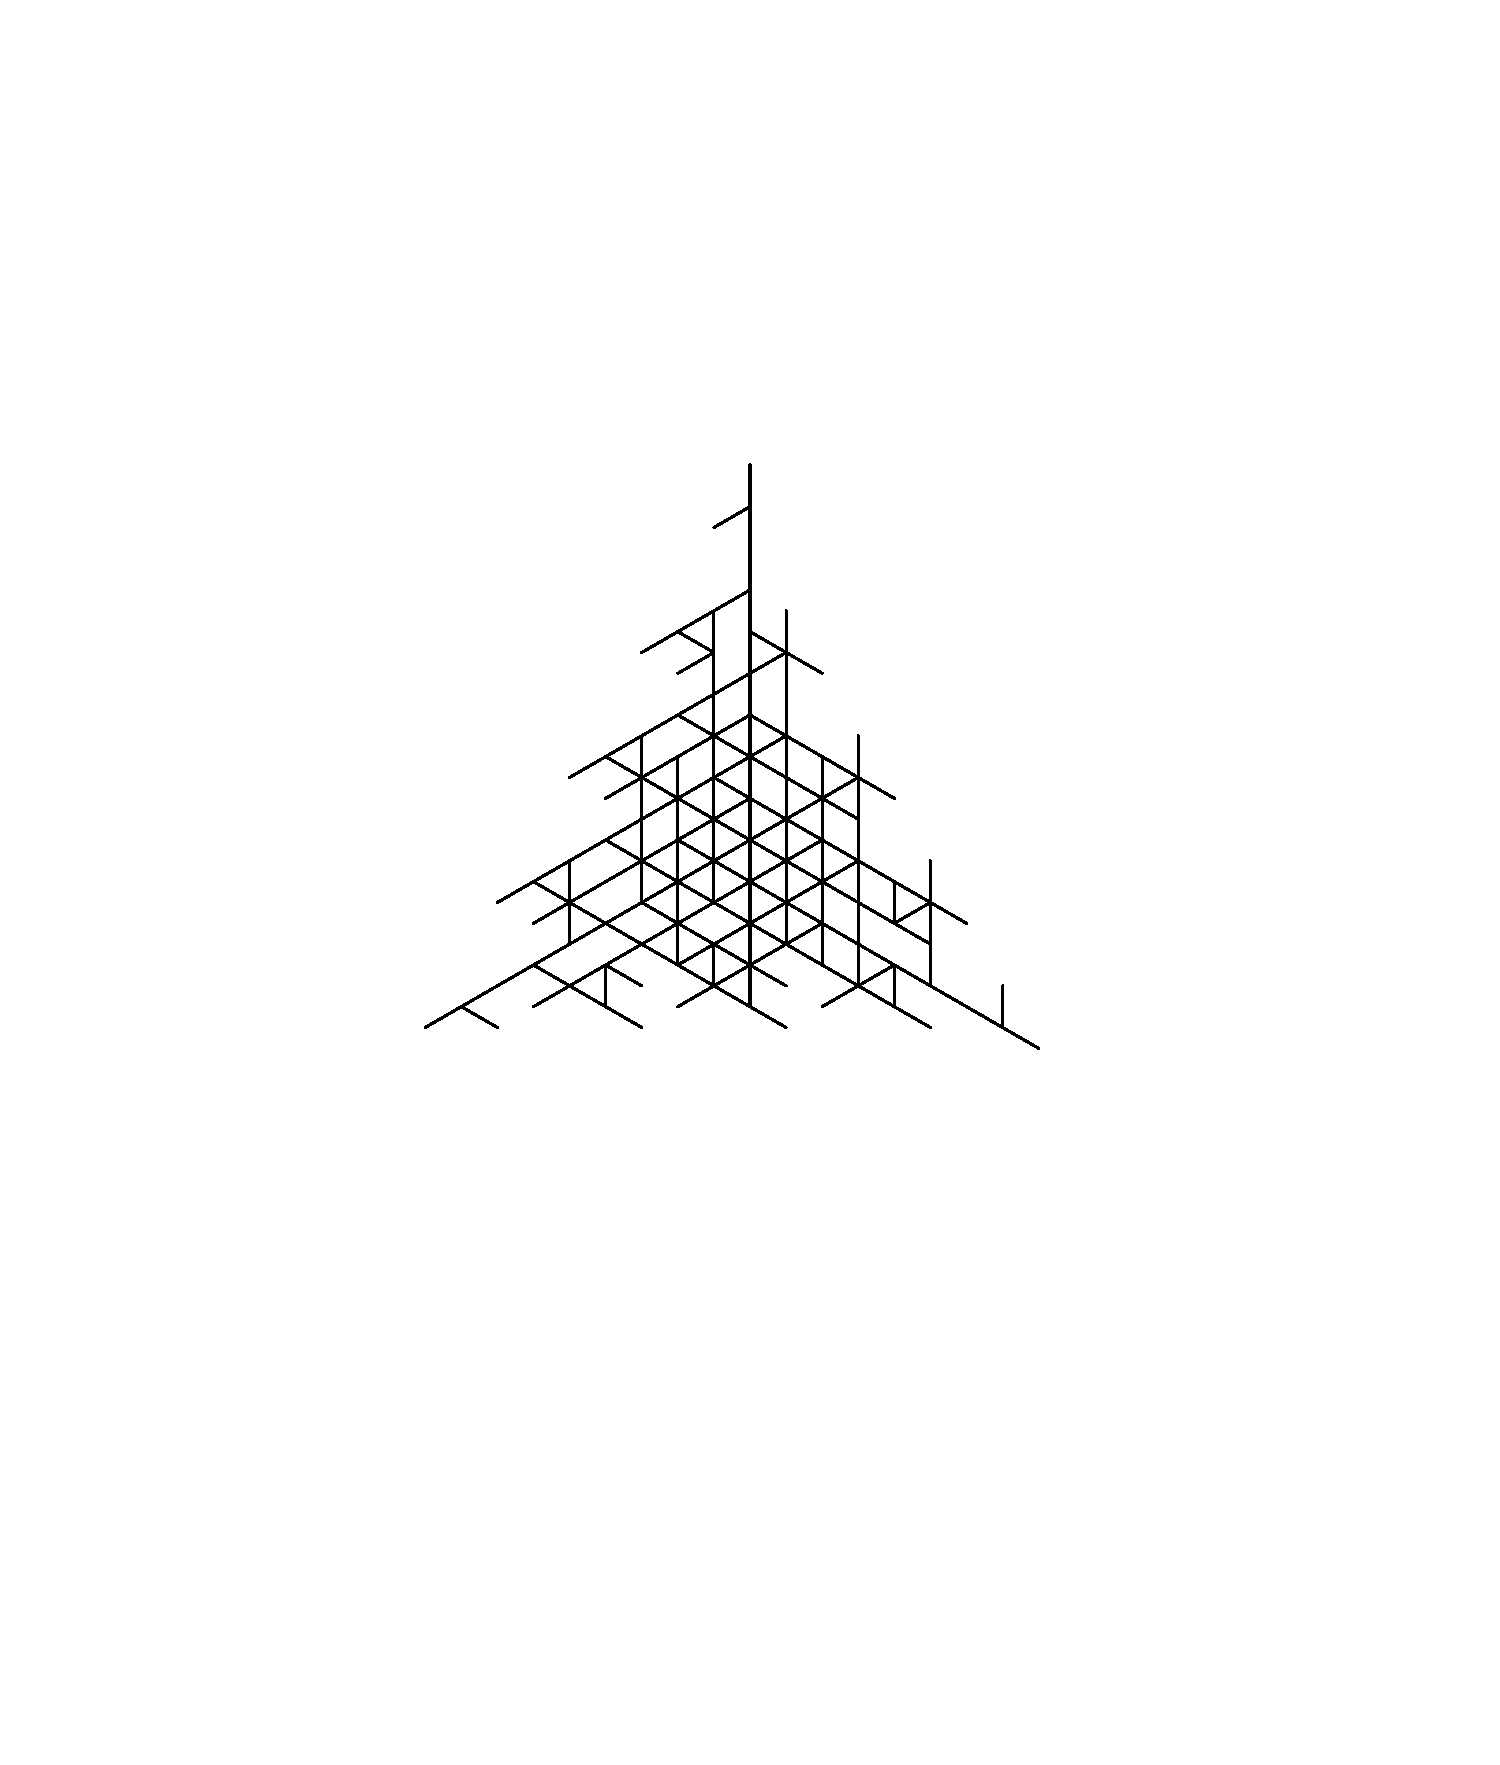
\includegraphics[clip=true, viewport=1in 4.5in 9in 9in, scale=0.6]{Images/Abstract1}
	\caption[Three-point Mirror]{Three-point Mirror\protect\footnotemark}
	\label {Acknowledgements1}
	\end{figure}
	\footnotetext{A; A $\rightarrow$ [F[–FA]FA]+A; $\theta$ = -120$^{\circ}$; Iterations = 5}
	
\chapter*{Dedication}
	\begin{center}
	
	To the unending search for understanding.\\
	
	\textit{for worlds. in worlds and over worlds}\\
	
	
	
	\end{center}
	
	
	\begin{figure}[h]
	\centering
	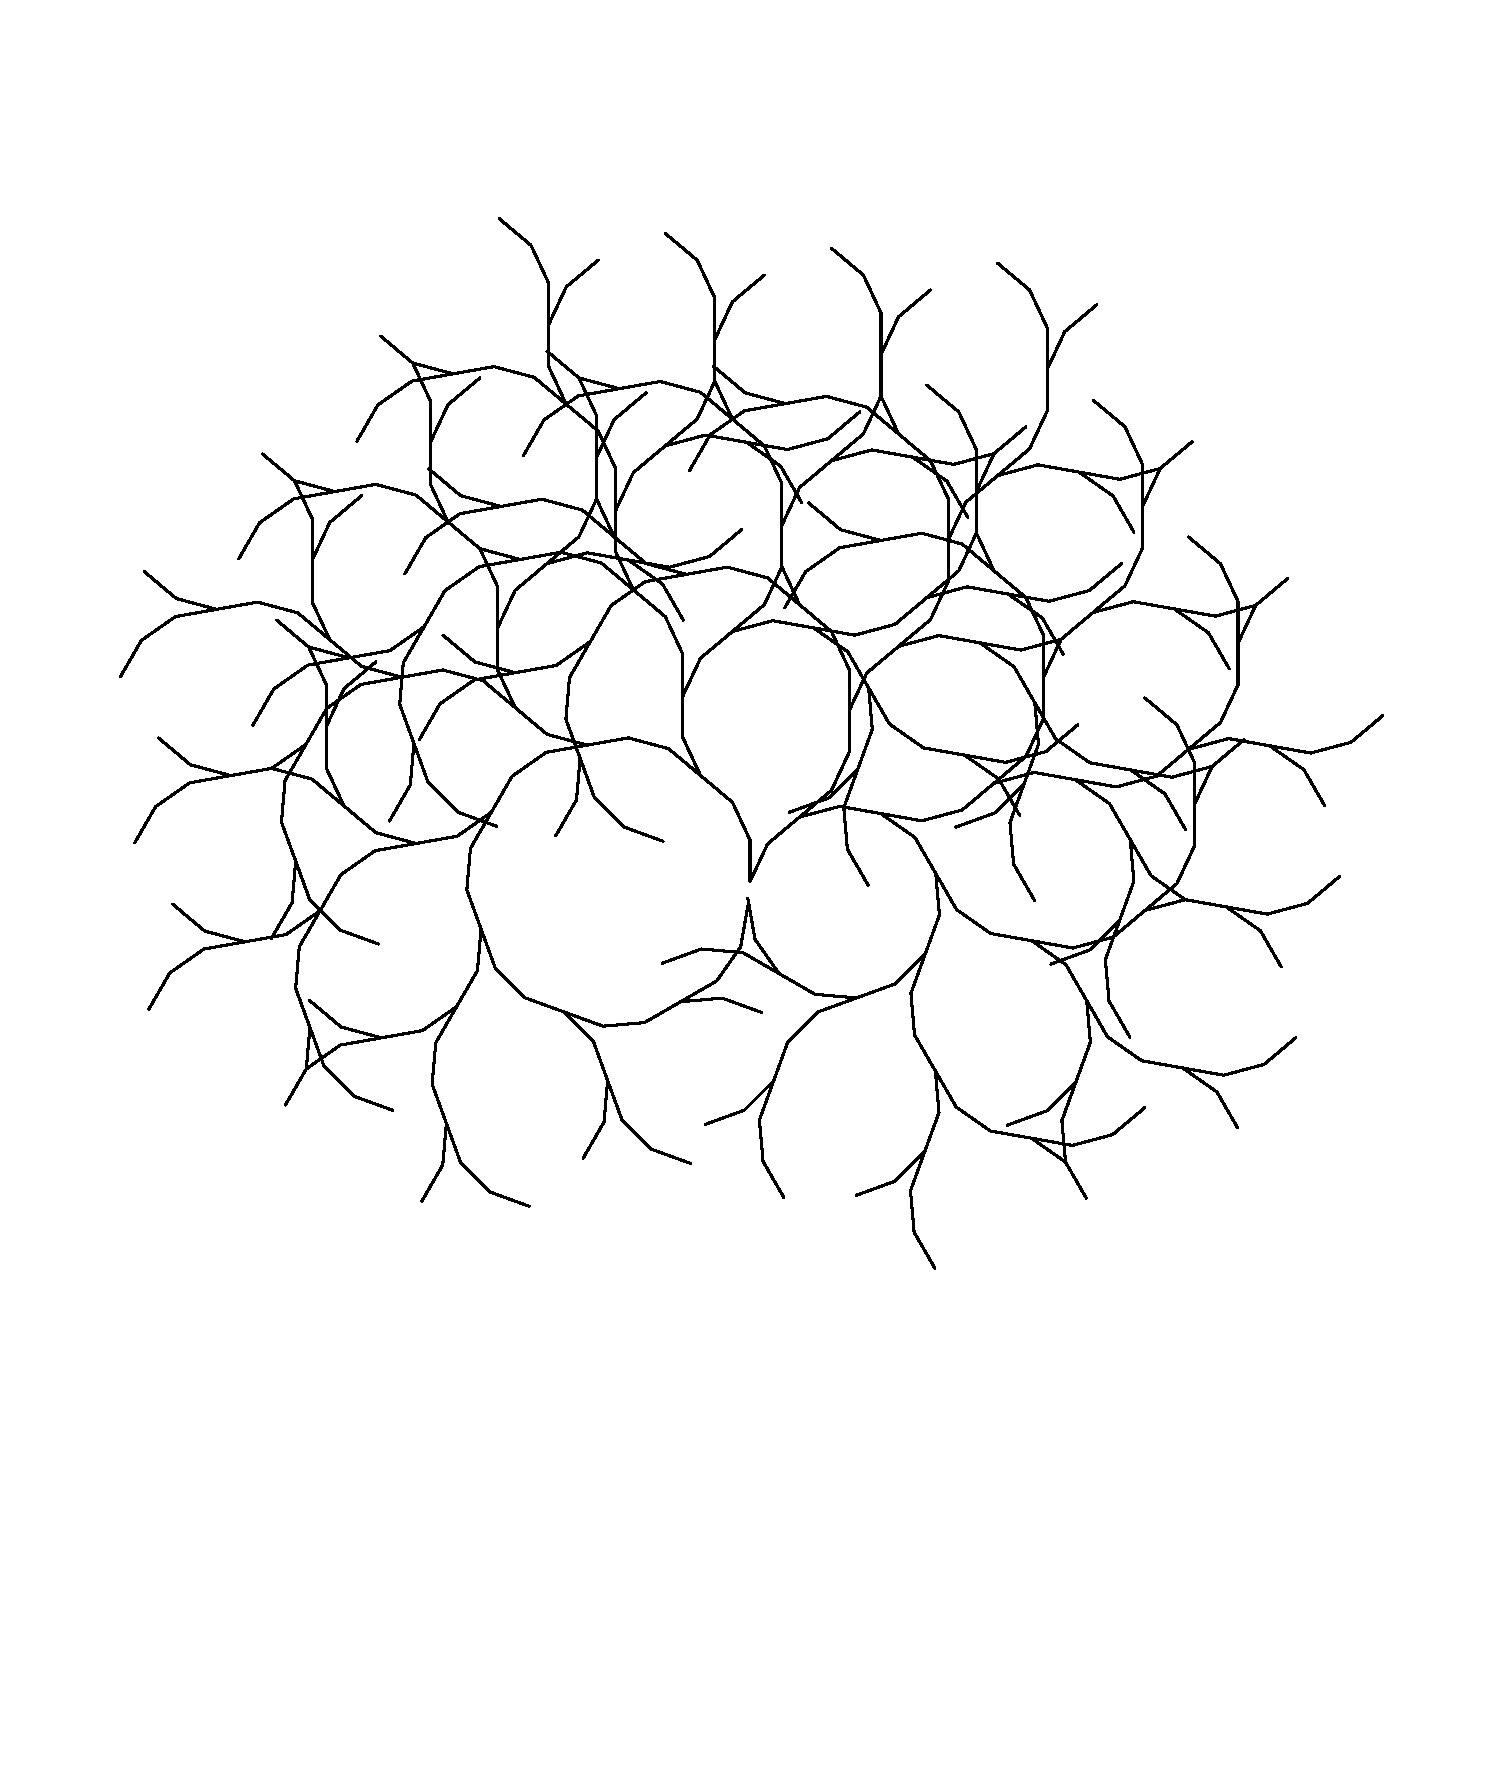
\includegraphics[clip=true, viewport=1in 3in 9in 10.5in, scale=0.6]{Images/Dedication1}
	\caption[Transcendent Spirals]{Transcendent Spirals\footnotemark}
	\label {Acknowledgements1}
	\end{figure}
	\footnotetext{A; A $\rightarrow$ [F+F+FA]–F–FA; $\theta$ = 25$^{\circ}$; Iterations = 7}

  \mainmatter % here the regular arabic numbering starts
  \pagestyle{fancyplain} % turns page numbering back on

\chapter*{Introduction: }
	%\addcontentsline{toc}{chapter}{Introduction}
	\chaptermark{Introduction}
	\markboth{Introduction}{Introduction}
	
%\textcolor{blue}{[Illustration of a simple L-System, perhaps just a fractal tree]}\\
	\begin{figure}[h]
	\centering
	
\includegraphics[clip=true, viewport=2.5in 5.5in 7.5in 8.5in, scale=1]{Images/Introduction1} % x-middle is 5, y-middle varies
	\caption[Classic Tree]{Classic Tree\footnotemark}
	\label {Introduction1}
	\end{figure}
	\footnotetext{A; A $\rightarrow$ F[+FA]–FA; $\theta$ = 32$^{\circ}$; Iterations = 5}


The world of Computer Science can seem like a wilderness, teeming with complex and specialized topics like Zero-knowledge proofs,\footnote{\cite{ZeroKnowledge1989}} NP-Completeness,\footnote{\cite{PvsNP1971}}  Finite State Machines,\footnote{\cite{FSMs2018}}  and the Halting Problem,\footnote{\cite{turing1936}}  but I hope to help show how approachable this discipline can be. Specifically at the hands of those from distant disciplines, like Anthropology, Economics, and Psychology, as well as the locals, pure Math, Bio, Chem, and Physics. The tool I introduce here will demonstrate the accessibility of this powerful, subtle, yet familiar discipline: Computer Science. The ideas that I employ in the program were named L-Systems, and their capabilities and beauty can astound.
	
Before we jump in, there are some things that must be said. This is a Computer Science Thesis, and so (essentially by necessity,) there will be code. I would like to keep this Thesis as accessible as possible to those who don’t code, and so I have tried to design it so that anyone with the ability to feel wonder and joy can find something of value between these covers. The code is accessible on my github, \textit{github.com/RJacobH/Thesis} as well as my website, \textit{rjacobh.github.io/website}. Some parts of the code of the central project will also be discussed at a later point in the thesis. However! I have included pictures at every moment I could, and I’d like to imagine that they tell enough of a story by themselves that to some extent the words are ultimately unnecessary.

%\textcolor{blue}{[An L-System that's mirrored across a horizontal line]}\\
	\begin{figure}[h]
	\centering
	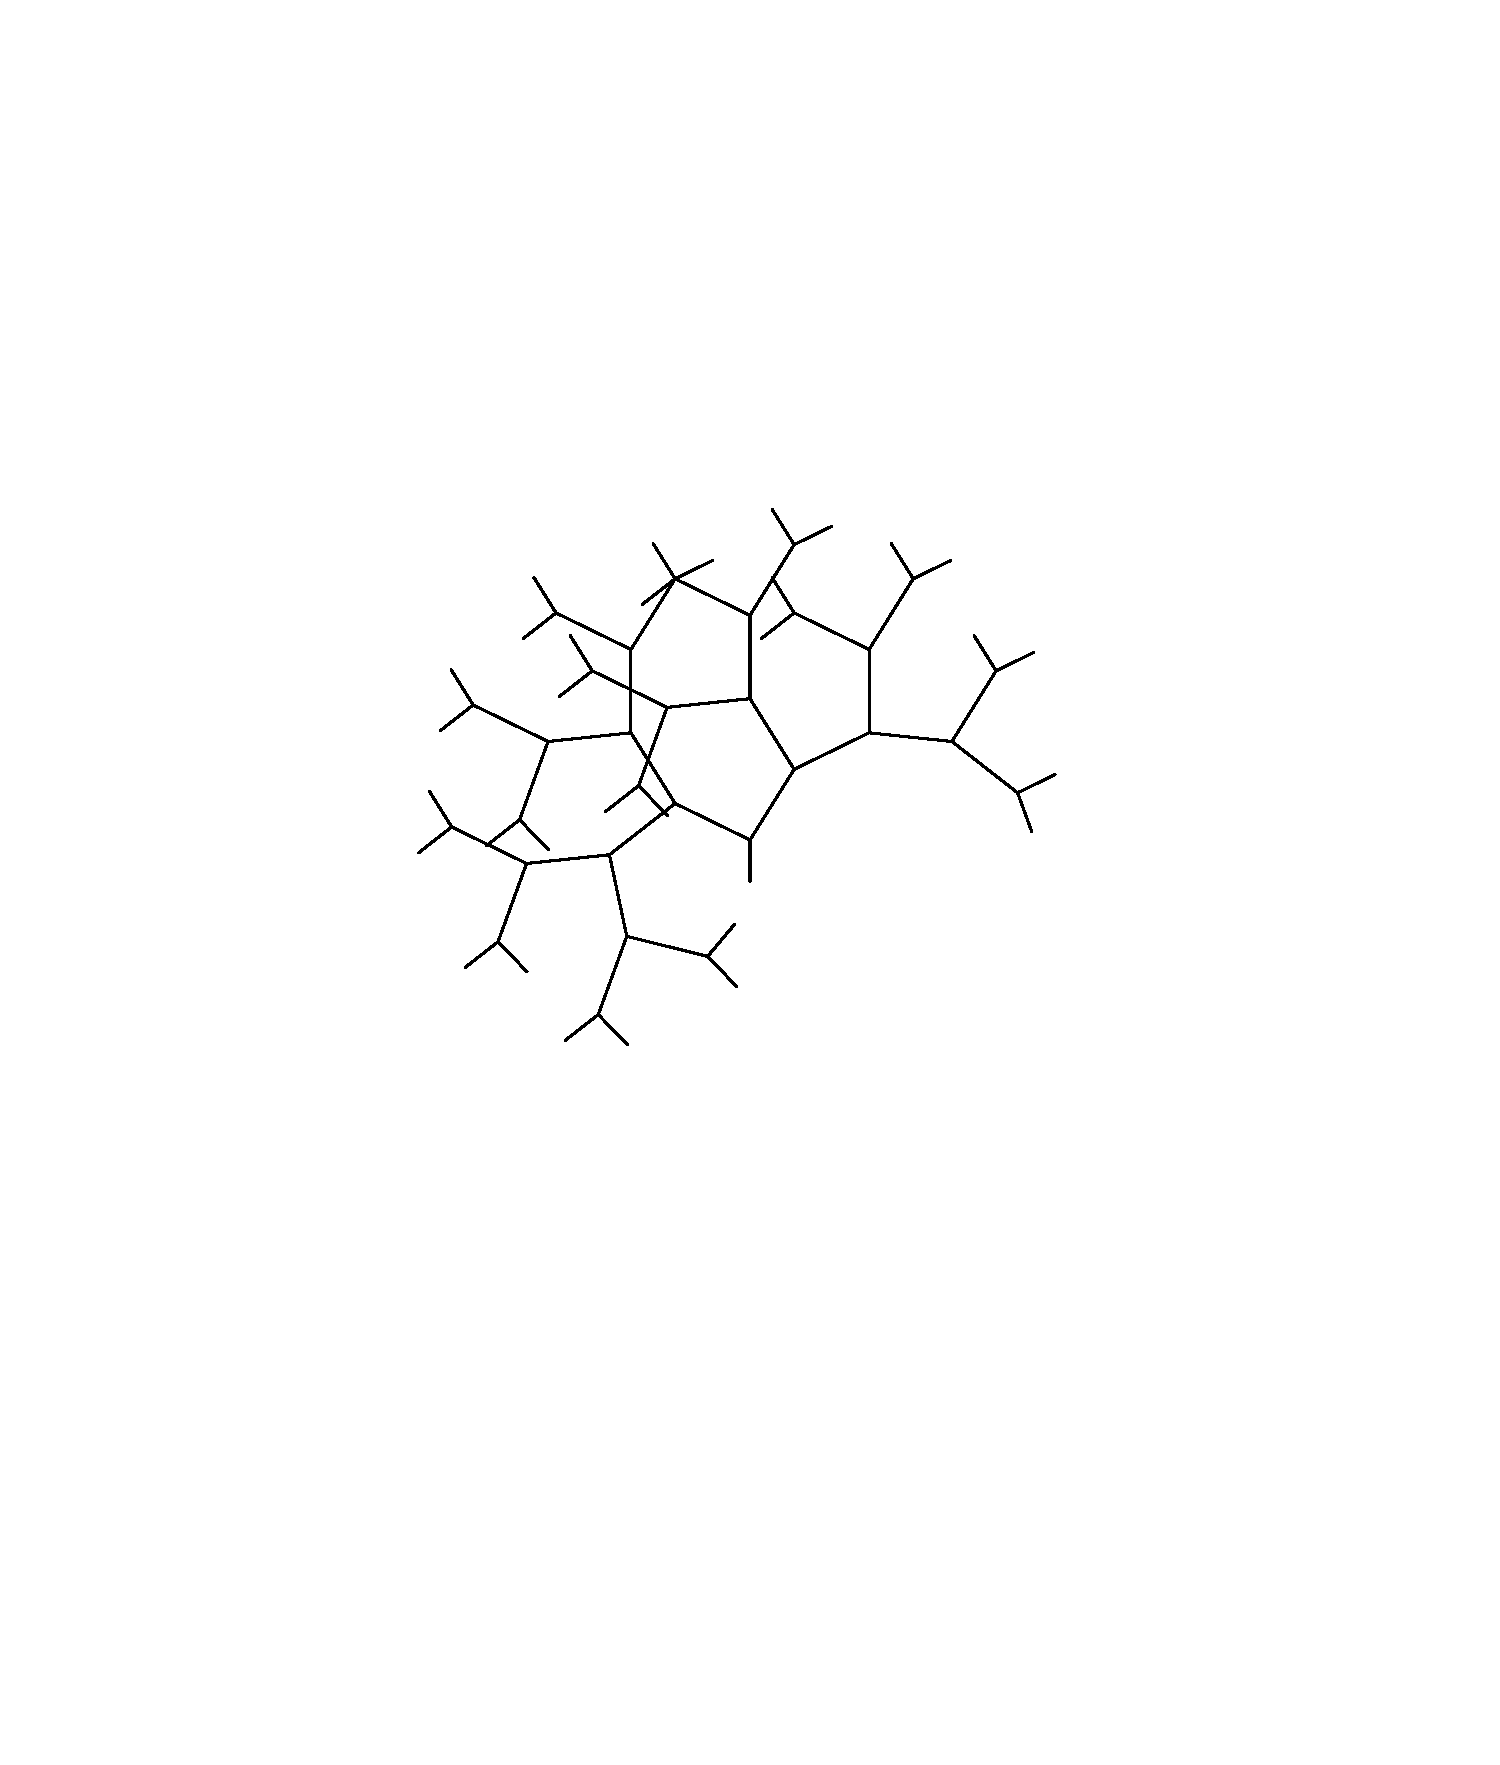
\includegraphics[clip=true, viewport=2.5in 4.5in 7.5in 8.5in, scale=0.75]{Images/Introduction2} 
	\caption[Tilted Classic Tree]{Tilted Classic Tree\footnotemark}
	\label {Introduction2}
	\end{figure}
	\footnotetext{A; A $\rightarrow$ F[++FA]–FA; $\theta$ = 32$^{\circ}$; Iterations = 5}

The structures that I will be discussing throughout this thesis are \textit{Lindenmayer Systems}, usually called \textit{L-Systems}. They are a type of ``rewriting" system that have a distinct visual flavor. Introduced by Aristid Lindenmayer in 1968\footnote{\cite{OG1967}} , they were first imagined as a framework for understanding the development of simple multicellular organisms. They were soon applied to larger systems, such as the structures of plants. A publication of Lindenmayer and others, \textit{The Algorithmic Beauty of Plants},\footnote{\cite{ABOP1990}} was written in 1990 and has been an invaluable resource for me in the formation of this thesis. It introduces L-Systems as a tool to celebrate and understand the beautiful complexity of plants, as well as to understand complex developments with limited arguments. Beyond this book, there have been a number of other vital resources in this process which I will discuss as they become relevant.

The images that appear throughout this thesis that look like Figure \ref{Introduction2} are specific examples of L-Systems. If you look at the footnotes that I've included with all of these images, you'll see a line of strange characters. I'll briefly describe here what those are, though I'll go into more detail in Section \ref{Understanding-through-Definitions}. Right now, all that's important to know is that they're fundamentally recipes for creating each of these L-Systems.\footnote{Beyond the discussion in Section \ref{Understanding-through-Definitions}, I direct you to Section \ref{Interpretations} to learn more about about the fifth part specifically.} If you'd like, you can create any of these L-System images on your own or in my program by following the recipe.  Also, unless otherwise noted, every image in this thesis was created or generated by me. The L-Systems that I show have almost always been created by one of my programs. 

L-Systems are fundamentally a collaborative topic, they cannot be understood from the perspective of just one discipline. An idea of their structure and abilities can only be sufficient if a variety of fields are consulted. I've tried to reflect this awareness in the form of my thesis as well as its content. I've tried to write something that would be as interesting for an artist to read as a computer scientist. If you're here for the pictures, please enjoy! But if you're here for the discussion of the systems that create those pictures, I urge you to stay and engage with some of the larger questions that I've asked about life, computers, and the place this thesis has in that discussion. But regardless of what brought you here, I hope you have a fun time looking through this thesis, and it warms my heart to know that there are people interested in this work which has captured by imagination so completely.


%\textcolor{blue}{[Illustration of an L-System, something that parallels the first one, and yet does something dramatically different (maybe the same image, just upside down? Inverted somehow?) Maybe just another cool L-System.]}


	\begin{figure}[h]
	\centering
	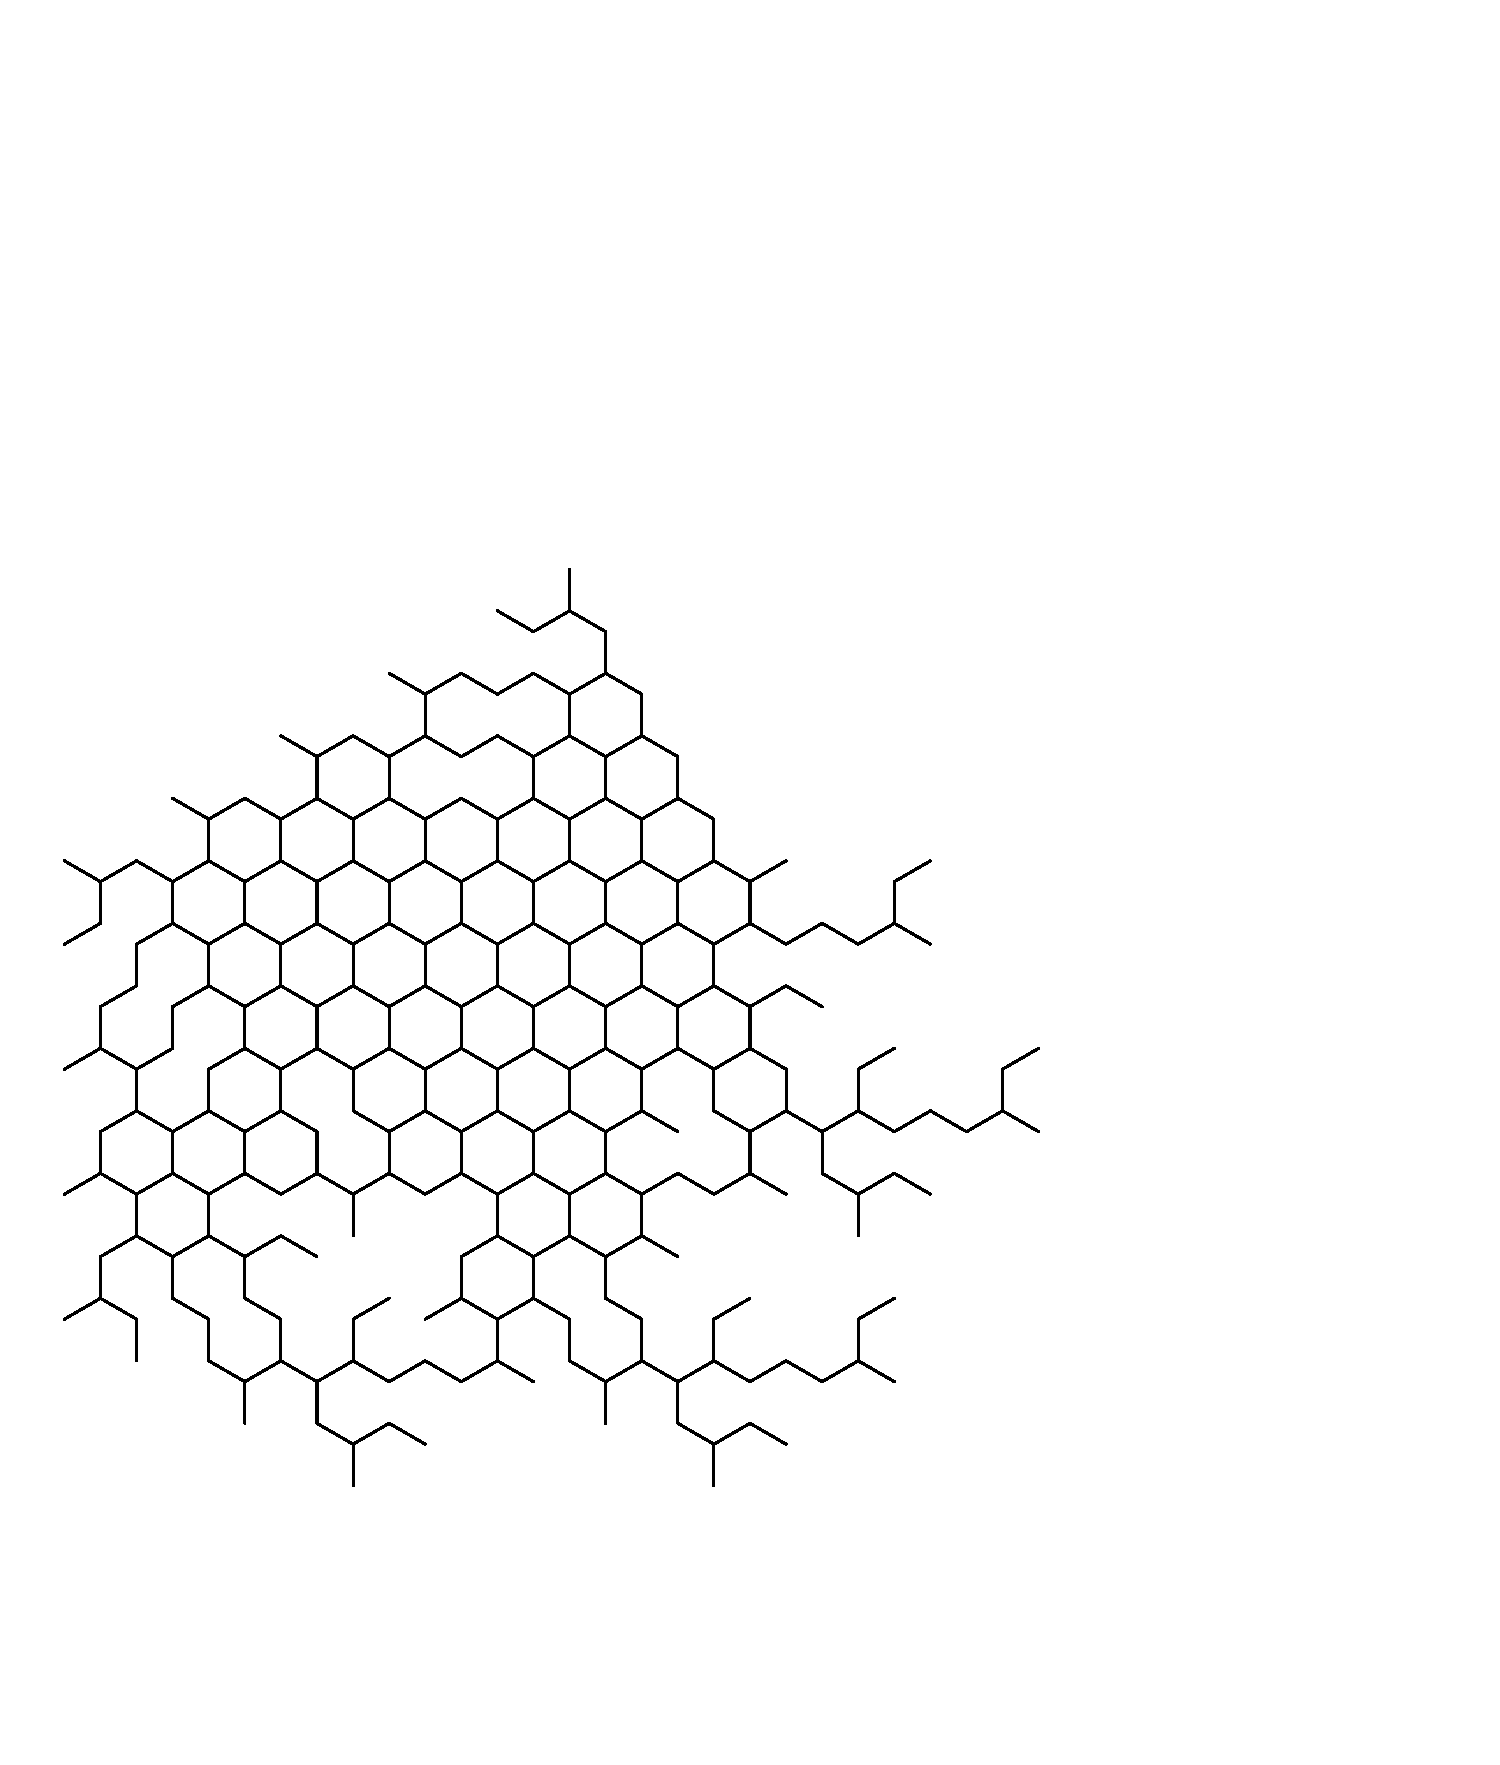
\includegraphics[clip=true, viewport=0in 1.5in 7.5in 8.5in, scale=0.4]{Images/Introduction3} 
	\caption[Aspirational Honeycomb]{Aspirational Honeycomb\footnotemark}
	\label {Introduction3}
	\end{figure}
	\footnotetext{A; A $\rightarrow$ +F[A+F–FA]–FA; $\theta$ = 60$^{\circ}$; Iterations = 5}

\section*{Motivations}

	The primary motivation, and the reason that I have become so personally invested in this topic, is the idea of \textit{pattern}. Patterns that I demonstrate with L-Systems and other generative arts appear at different scales throughout life, the world, and our universe. I was in near constant conversation with my friends and acquaintances in other disciplines while I was writing this, and I was amazed at how often questions of self-reference, universality, and beauty from simple rules arise in areas beyond just Computer Science. % I want specific examples, but I don't have any right now
	
	%\footnote{We can see } %I hope to draw in Economists and Anthropologists in addition to Physicists and those from other areas with discussion of patterns that appear in the structures of society and social organization, and which can be illustrated to some extent with the methods that I outline here.

%\textcolor{blue}{[Mathy L-System (Something Fractal)]}\\
	\begin{figure}[H]
	\begin{subfigure}{0.5\textwidth}
		\centering
		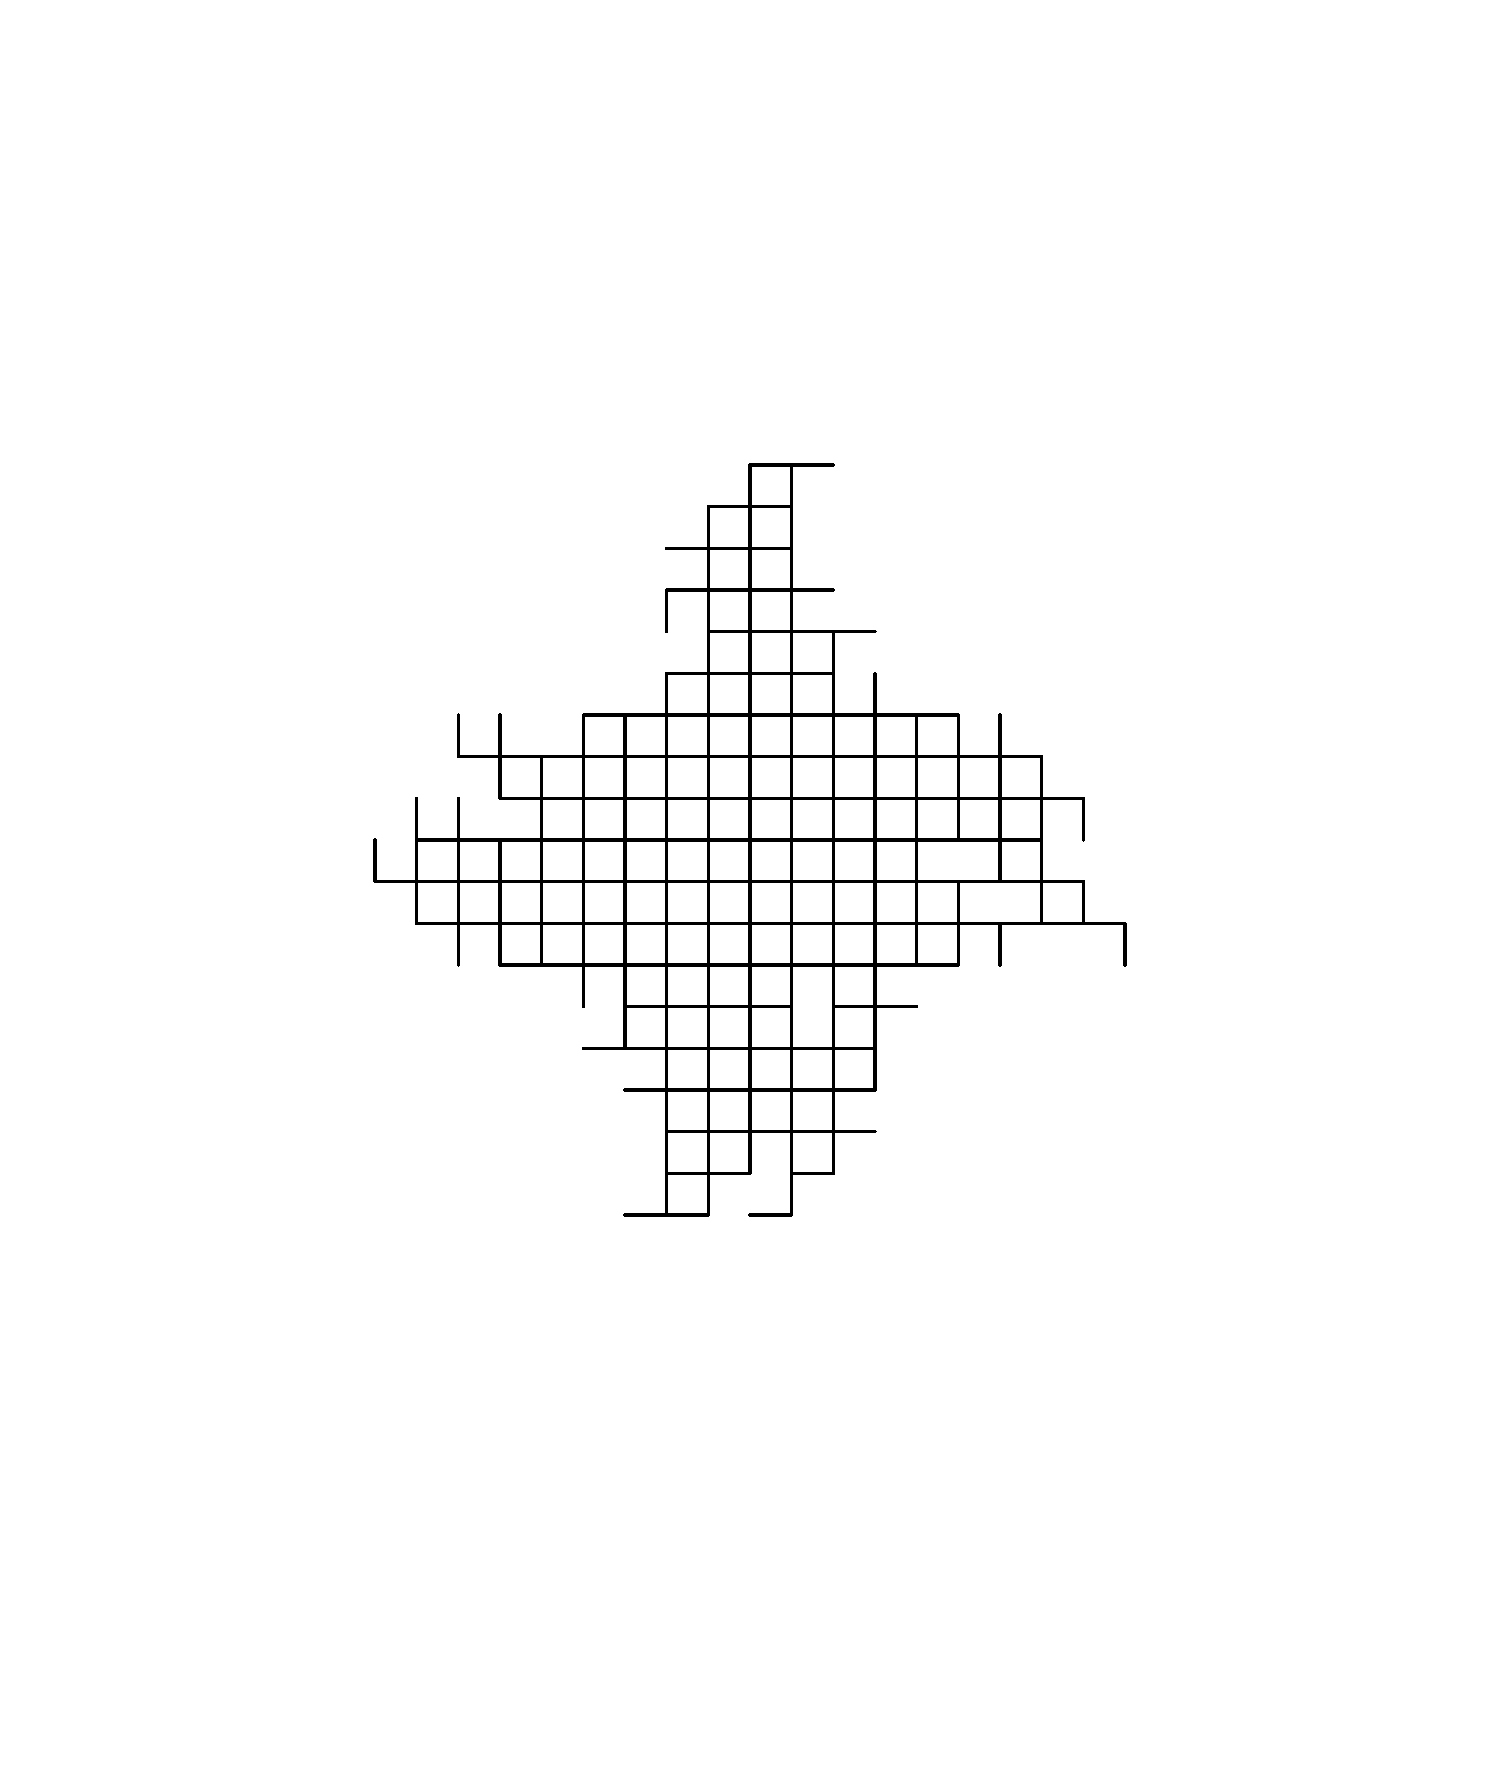
\includegraphics[clip=true, viewport=1.35in 3.5in 9.35in 9in, height=0.8\textwidth]{Images/Motivations1A}
		\caption[90 degrees]{90 degrees\footnotemark}
		\label {Motivations1A}
	\end{subfigure}
	\begin{subfigure}{0.5\textwidth}
		\centering
		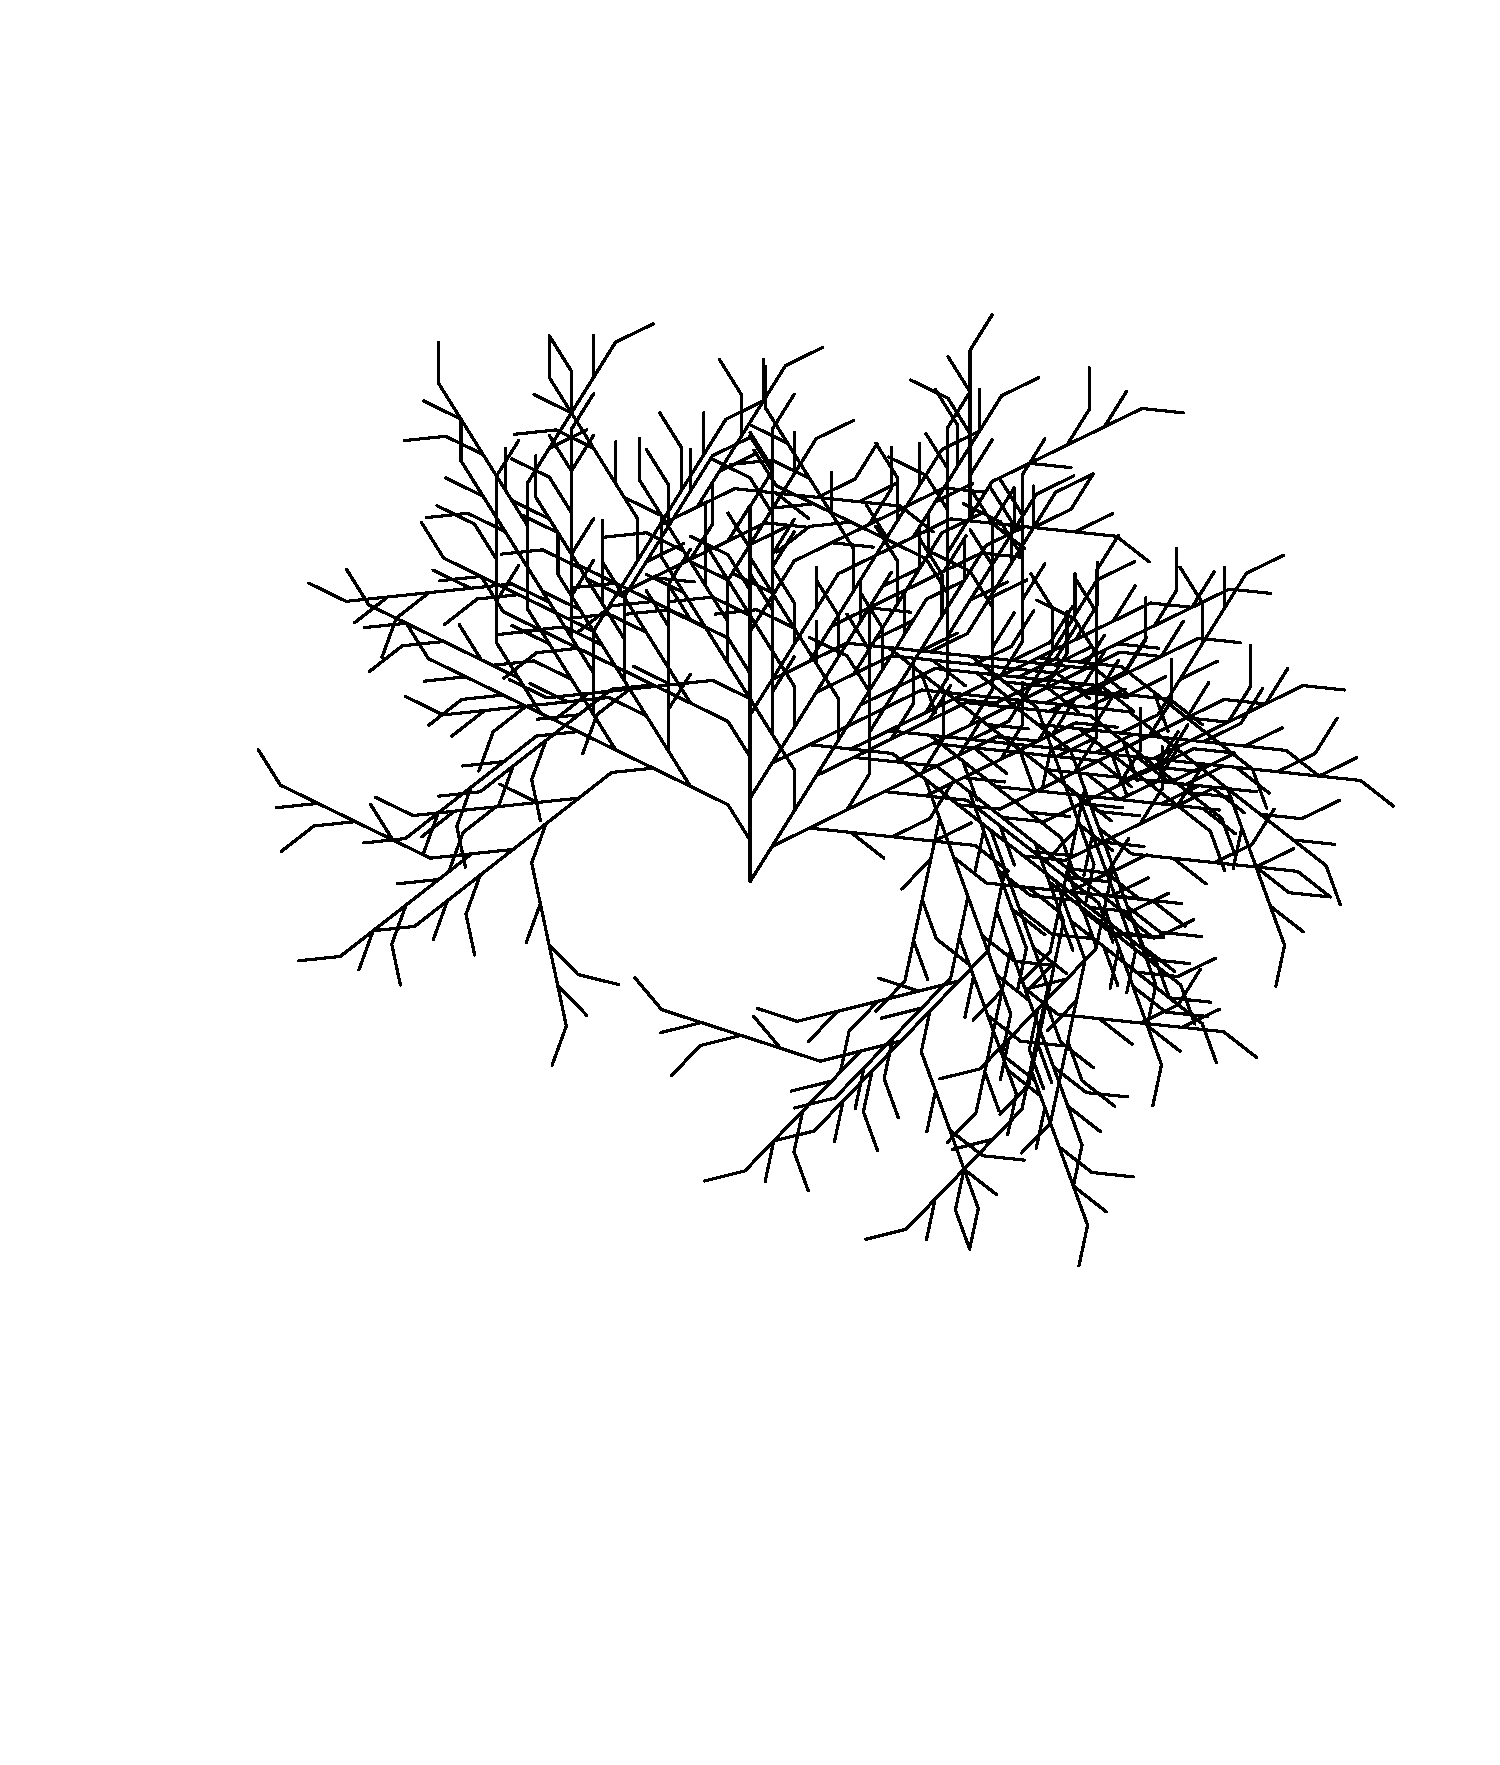
\includegraphics[clip=true, viewport=1in 3.3in 9in 10in, height=0.8\textwidth]{Images/Motivations1B}
		\caption[32 degrees]{32 degrees\footnotemark}	
		\label {Motivations1B}
	\end{subfigure}
	\caption[Nearly Identical L-Systems]{Nearly Identical L-Systems}
	\label{Same}
	\end{figure}
	
	\addtocounter{footnote}{-1}\footnotetext{A; A $\rightarrow$ [F[+F+FA]FA[F–FA]+FA]-FA; $\theta$ = 90$^{\circ}$; Iterations = 4}
	\addtocounter{footnote}{1}\footnotetext{A; A $\rightarrow$ [F[+F+FA]FA[F–FA]+FA]-FA; $\theta$ = 32$^{\circ}$; Iterations = 4}


	The second main motivation is the simple beauty of many of the patterns that emerge when working with L-Systems. This is the motivation that I imagine might be the most interesting to artists, be they visual artists or otherwise. It is also the reason I became aware of L-Systems and their relatives in the first place, so it is as essential a part of this story as the first motivation. It should be noted that it feels like the division between these fields is not nearly as dramatic as one might imagine. There are varied connections between the Art aspects of this work and the Computer Science and Math aspects, some of which I will explore later in the thesis. 
	
	\begin{figure}[h!]
	\centering
	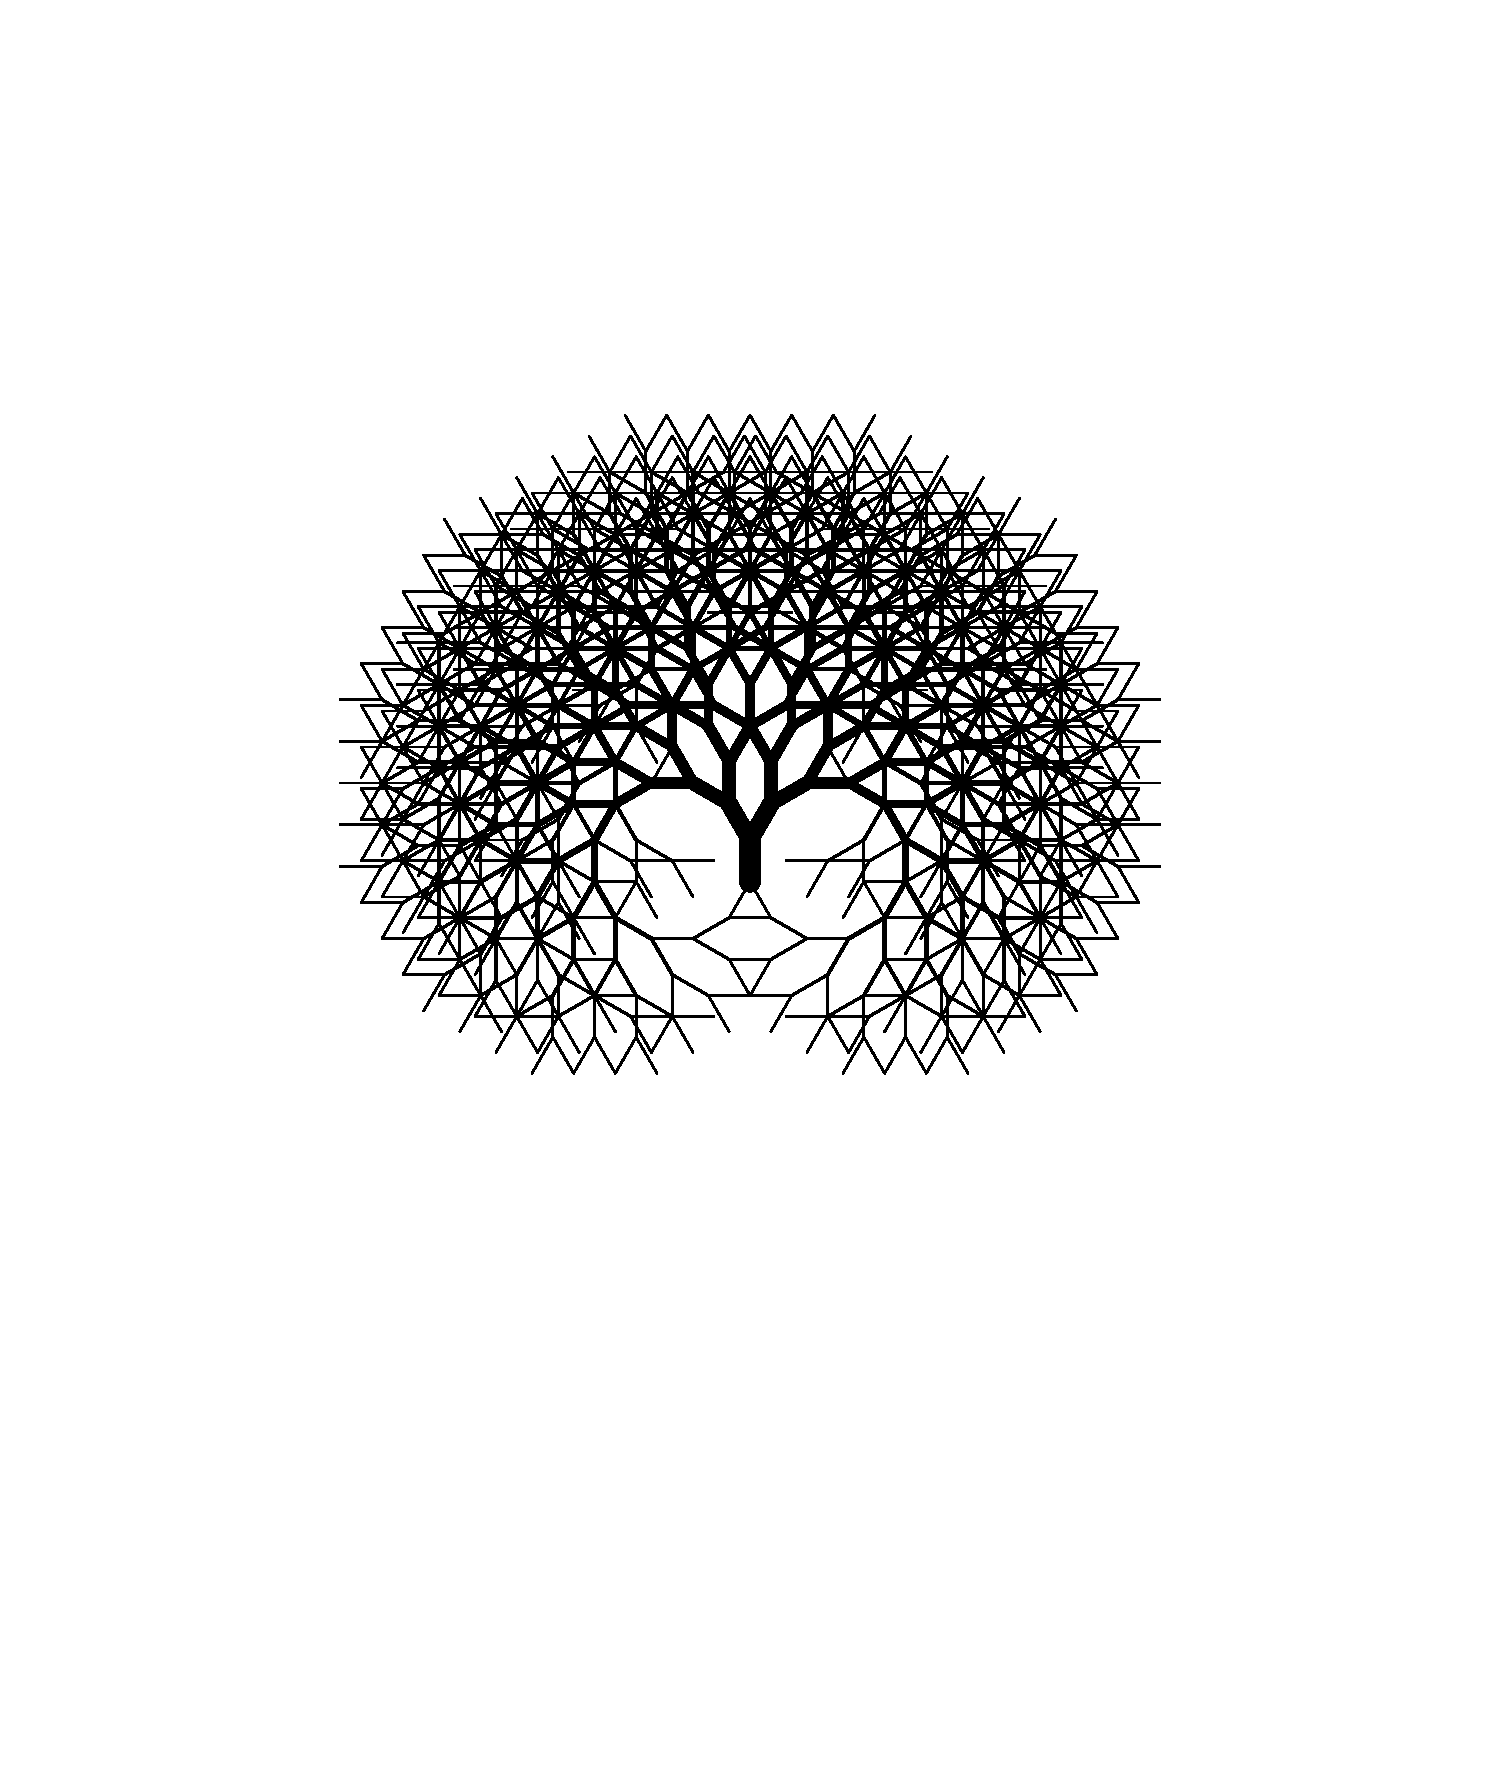
\includegraphics[clip=true, viewport=1in 1.5in 9in 8.5in, scale=0.3]{Images/Motivations2}
	\caption[Fishhook]{Fishhook\footnotemark}
	\label {Motivations2}
	\end{figure}
	\footnotetext{A; A $\rightarrow$ +F[A]F–FA--FA; $\theta$ = -156$^{\circ}$; Iterations = 6}
	
	The third motivation is tied in with a philosophical understanding of these structures. As I delved deeper into L-Systems, I came across the claim that these structures themselves were \textit{alive}.\footnote{\cite{theory2004}} This felt absurd, but I understood how a person could see life within the symmetry. I found that it was extremely difficult for me to draw the line between living and non-living matter without the choice feeling somewhat arbitrary. A conventional definition, that the smallest unit of life is the cell due in part to its ability to self-replicate, felt insufficient. These structures I was in the process of investigating do replicate themselves to some extent, so why shouldn't they live? These questions on the nature of life stuck with me, and I found myself asking the same questions of life in the context of other machines. I ask address larger issues of the place of machines in the creation of art and the creative process. It also feels like these questions about the border between living and non-living things are essential when we're experiencing what may be the first great wave of AI systems.

	\begin{figure}[h]
	\centering
	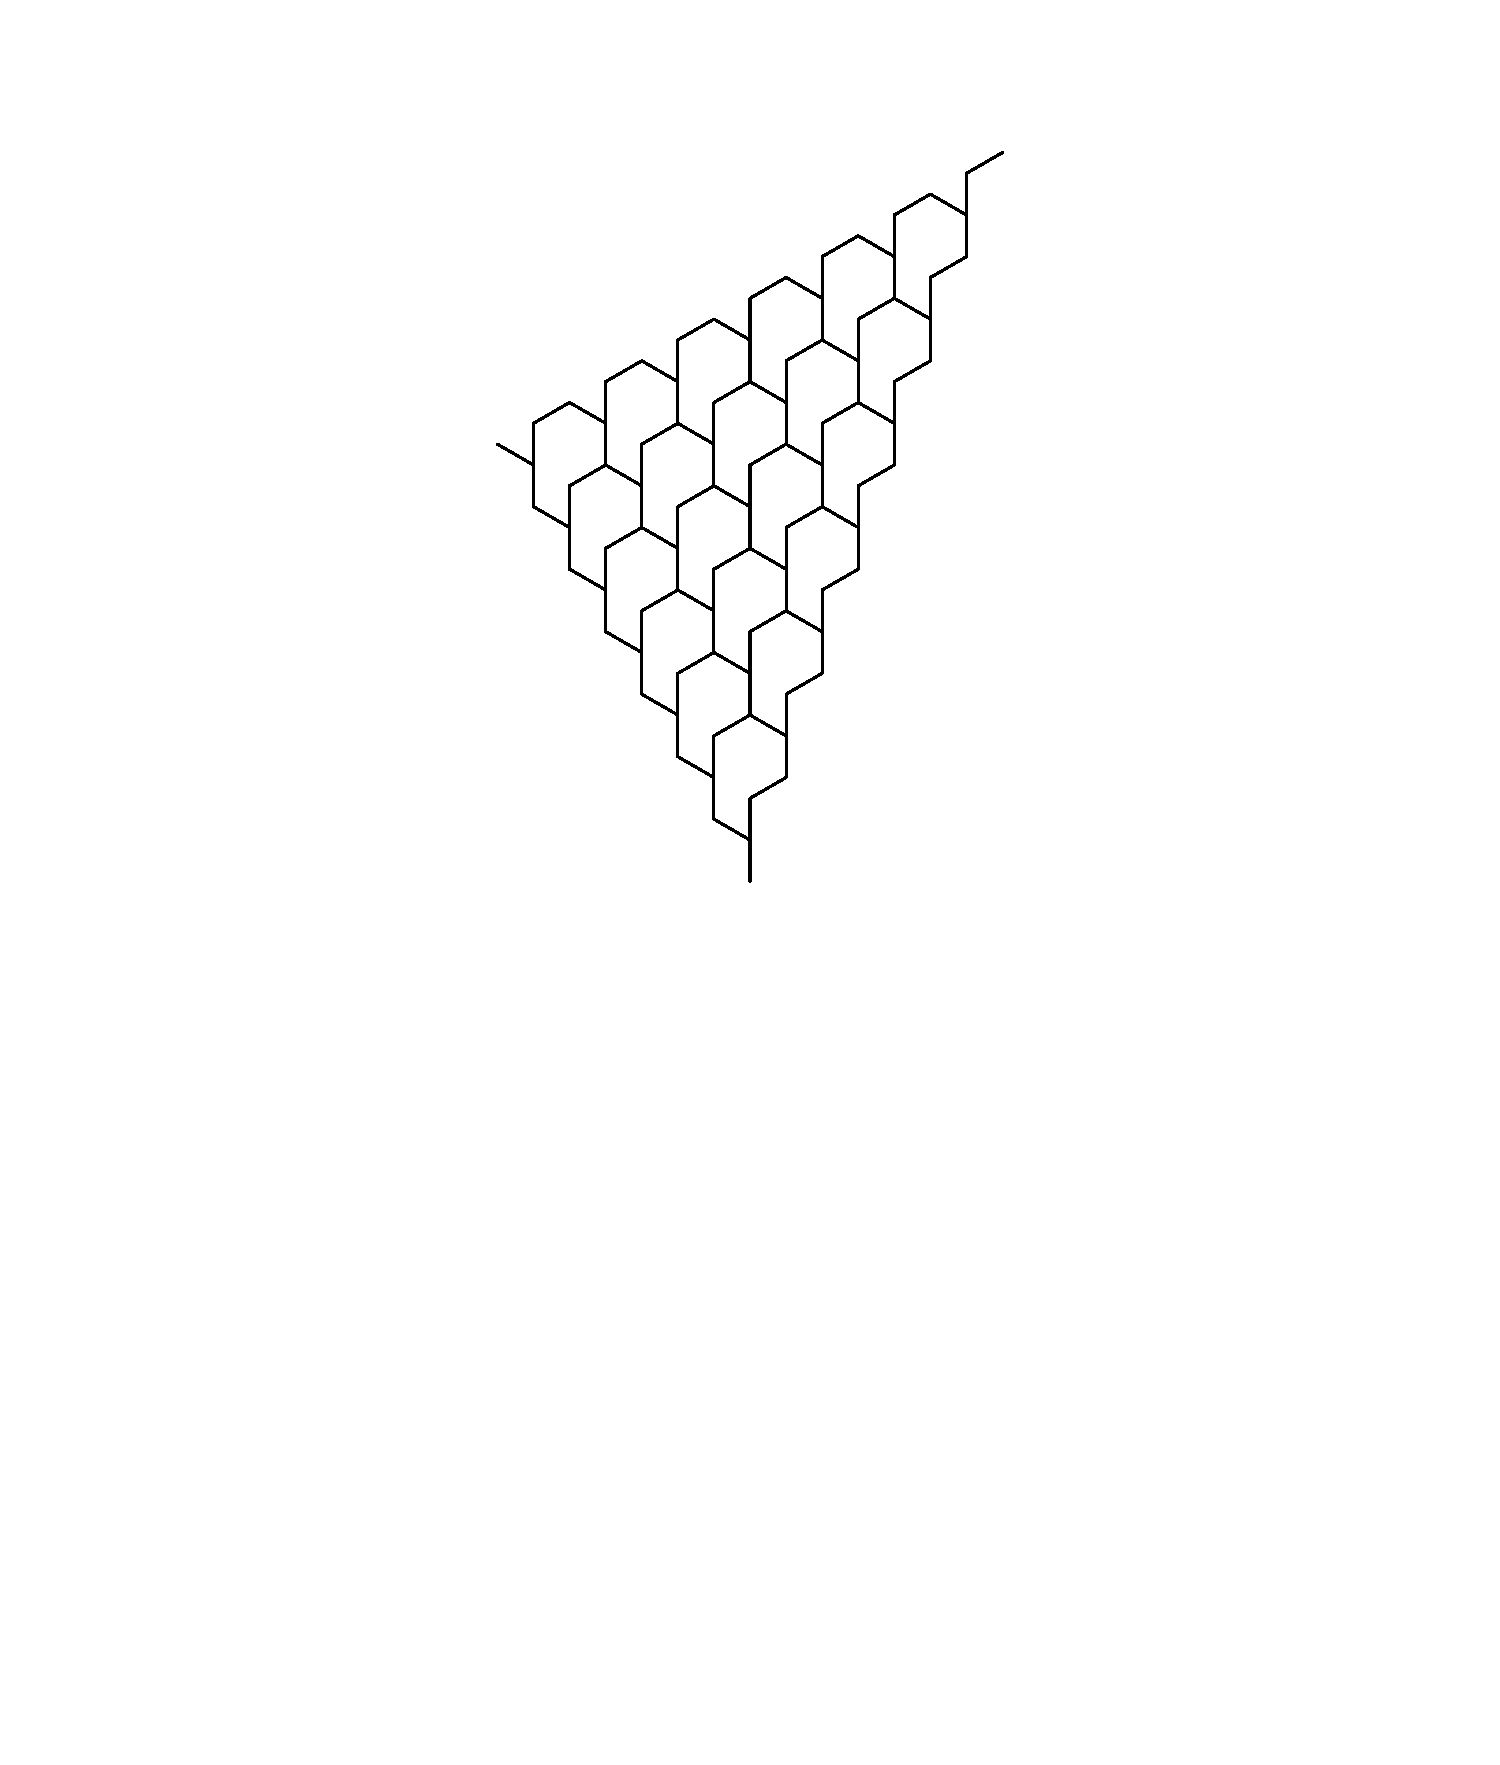
\includegraphics[clip=true, viewport=1in 6in 9in 11in, scale=0.4]{Images/ThePathWeWillFollow1}
	\caption[Not Quite 3d]{Not Quite 3d\footnotemark}
	\label {Motivations3}
	\end{figure}
	\footnotetext{A; A $\rightarrow$ F[+F–A]F–F+A, B $\rightarrow$ F–FA; $\theta$ = 60$^{\circ}$; Iterations = 7}

	This thesis does not aim to answer any of these questions. I ask them and suggest that they are important questions to be asking, but mainly state them so that you see what I've been thinking about as part of this process. I present my research as an open book for you to read and find whatever is valuable for you. Although, I do assert the importance of L-Systems and other simple, powerful tools that a person can hope to understand, especially in a time when so many of the systems that control our lives are invisible to us. These questions have been a foundational piece of my work, and have shaped the development of this thesis as much as the content itself.
	
	I hope that L-Systems will find a broader audience, either as a result of the work that I’ve done here or as part of some other exploration of their abilities. This came to be a motivating project for me for more reasons beyond those outlined above, and I imagine that someone who sets new eyes on this work could see it in a way I never could have imagined. I go into more detail near the end of the thesis about what I believe I have contributed to the conversation around L-Systems and their relatives, as well as what I believe the program I wrote could do if more time is given to its evolution.
	
	%\textcolor{blue}{[A long, thin L-System which stretches from one side of the page to the other]}
	

	
\section*{The Path We Will Follow}

	The first thing I will do in this thesis is formally introduce L-Systems. I will give different perspectives on the construction of these systems to help the reader see that they are incapable of being understood from any single one of these perspectives. The only way to get the whole picture is to know that a single explanation will always be insufficient.

	From there, I'll begin to demonstrate the abilities of L-Systems. I've chosen to display them as a 2d or 3d visual structure, though there are other ways to express them, which are discussed in Section \ref{Interpretations}. While they can look compelling, the process of creating them has been hard to access and engage with for those outside of Computer Science. I wanted to make it so that people with any knowledge about them could play with them. I wanted to bring wonder and teach about these systems, so I wrote a program to do just that. I describe the structure of the program, some steps I took in its development, and how to use it, and I direct interested readers to try the program themselves. How to access the program is detailed in Section \ref{Using-the-L-Systems-Explorer}.% The link to the program is here... [share the link]
	
	%\textcolor{blue}{[Some simple L-System (maybe one with step-like features?)]}\\
	\begin{figure}[h]
	\centering
	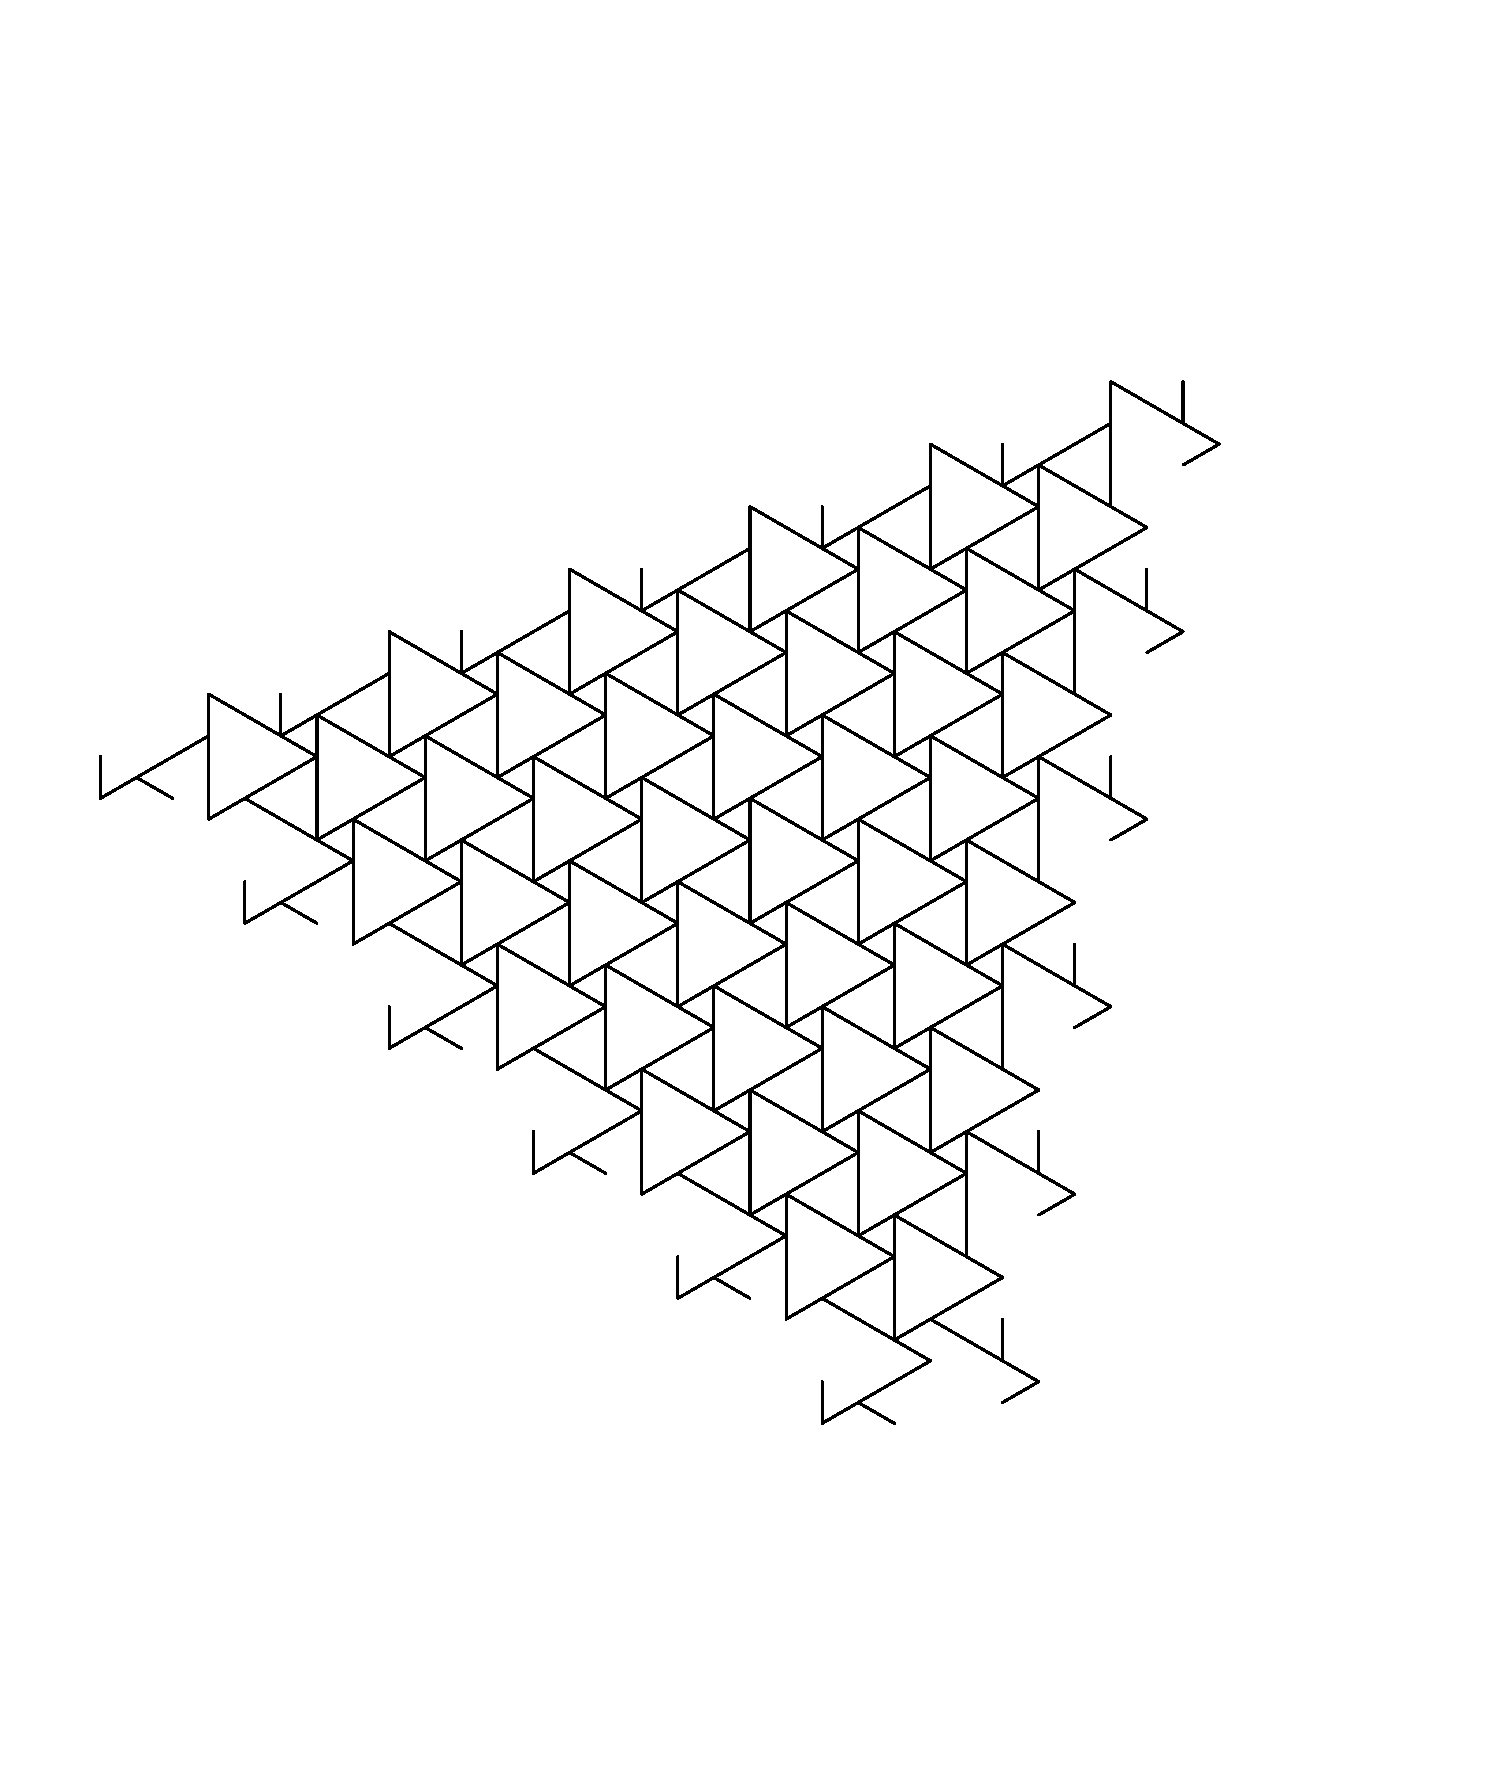
\includegraphics[clip=true, viewport=0.5in 2in 9.5in 10in, scale=0.4]{Images/ThePathWeWillFollow2}
	\caption[Triangle Heaven]{Triangle Heaven\footnotemark}
	\label {Motivations3}
	\end{figure}
	\footnotetext{A; A $\rightarrow$ F[F+FA]–FA; $\theta$ = -120$^{\circ}$; Iterations = 12}
	
	In Section \ref{GenerativeArt} I go on to talk about Generative Art and the broad crossover between Art and Computer Science that has fueled this thesis and the work of many other contemporary artists. I talk about some of my earlier explorations into L-Systems and Generative Art, and connect those experiments with the resulting thesis. After that, I talk about some of the questions I've asked during this research, in Computer Science and in areas beyond. I place this thesis within its historical moment and suggest some broad extensions that aren't direct continuations of this work.
	
	I explore the origin of L-Systems and their early connection to simulations of living structures, especially those of plants. \textit{The Algorithmic Beauty of Plants},\footnote{\cite{ABOP1990}} or \textit{ABOP}, written by Aristid Lindenmayer, their progenitor, and Przemyslaw Prusinkiewicz, has been an invaluable resource for me in the development of this thesis. In this section, I touch on some of the ways that this book guided parts of my research and helped me make judgement calls about what I'd be focusing on. There are some types of L-Systems that I don't include in my program. This is the point where I talk about those types of L-Systems and why I decided to not include them.
	
	%\textcolor{blue}{[Some of the images from ABOP]}
	
	\begin{figure}[h]
	\centering
	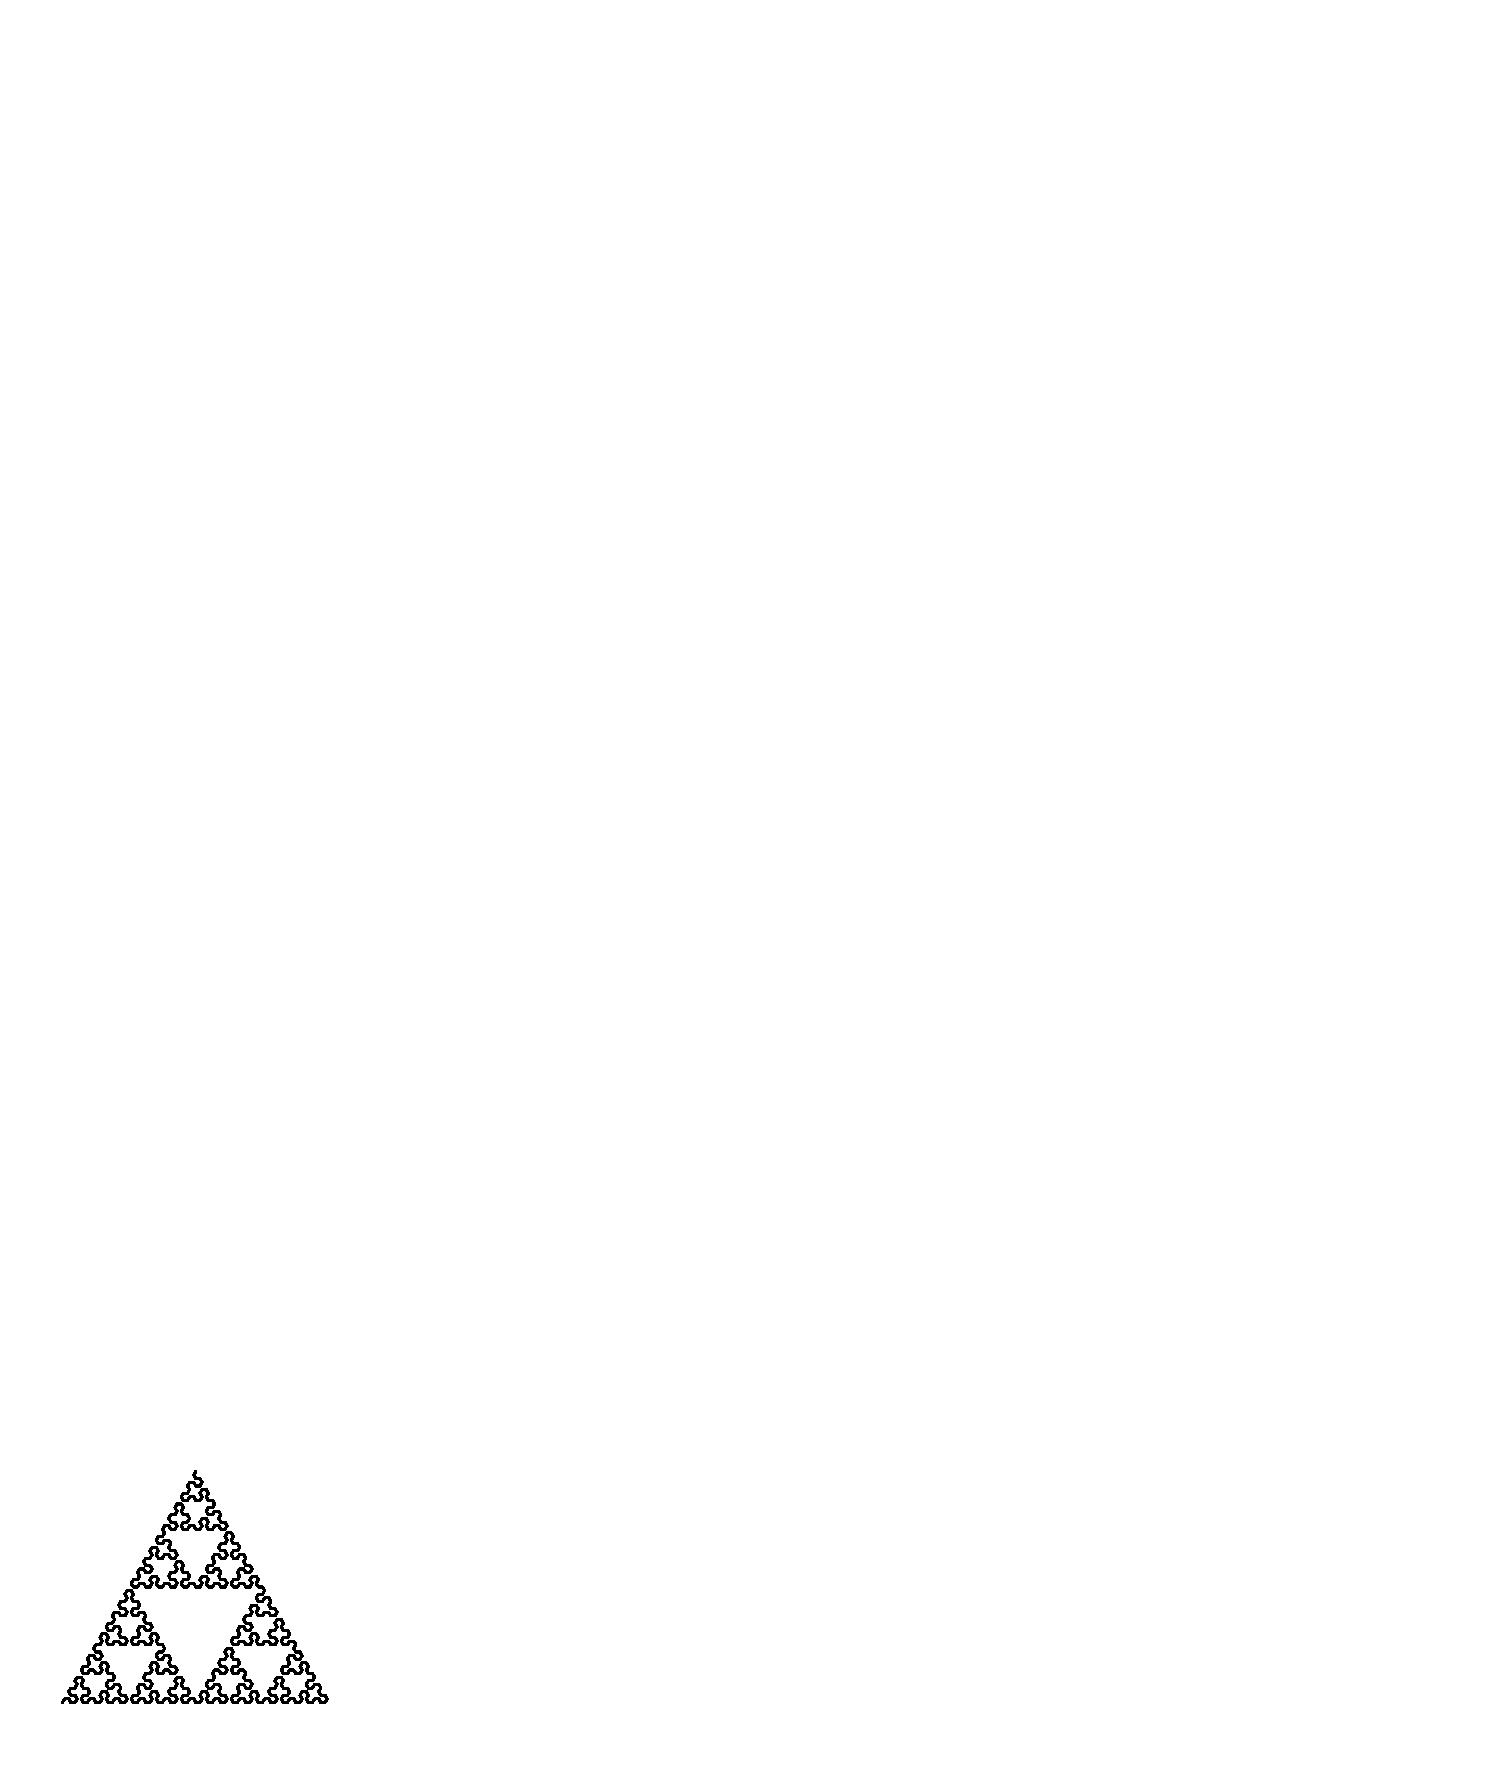
\includegraphics[clip=true, viewport=0in 0.3in 2.5in 2in, scale=1.4]{Images/Sierpinski} % x-middle is 5, y-middle varies
	\caption[Sierpinski Gasket]{Sierpinski Gasket\footnotemark}
	\label {Sierpinski}
	\end{figure}
	\footnotetext{A; A $\rightarrow$ B+A+B, B $\rightarrow$ A–B–A; $\theta$ = 60$^{\circ}$; Iterations = 6 (A and B draw)}
	
	In Section \ref{Extensions} I discuss possible extensions of the program. Some of these extensions are little more than user interface changes while others might require underlying structural changes to function. In order to more competently think about the second of these goals, I reference the choices I've made regarding the content of \textit{ABOP}. I address some of the considerations that might have to be made in order to introduce some of the structures in \textit{ABOP} to my own program.
	
	\begin{figure}[h]
	\centering
	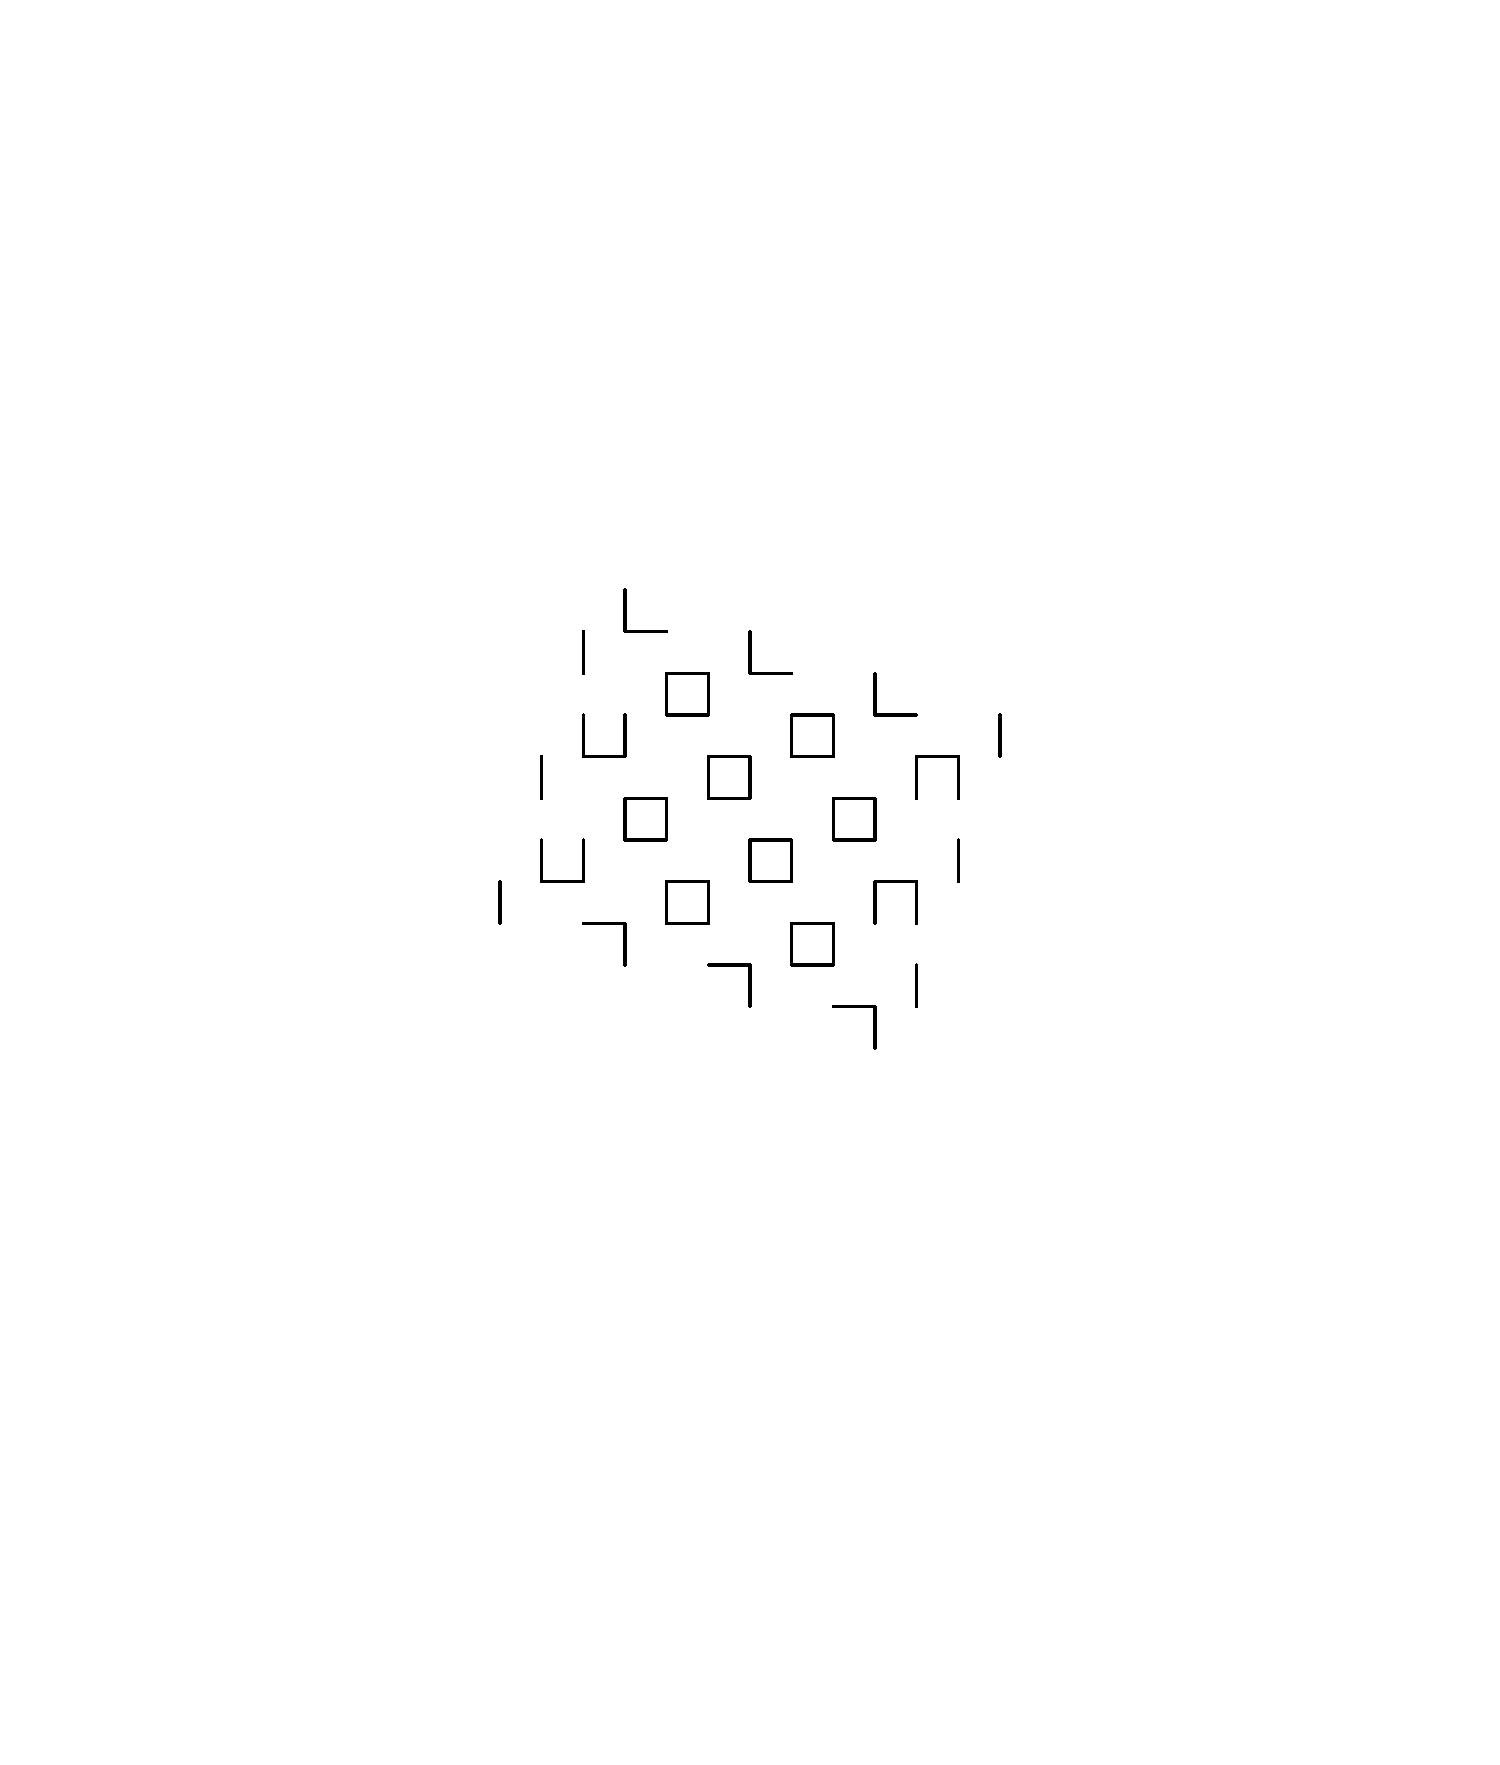
\includegraphics[clip=true, viewport=1in 4.5in 9in 8in, scale=0.5]{Images/ThePathWeWillFollow3} % x-middle is 5, y-middle varies
	\caption[L-Swiss]{L-Swiss\footnotemark}
	\label {Holey}
	\end{figure}
	\footnotetext{A; A $\rightarrow$ F[+A]f–A; $\theta$ = -90$^{\circ}$; Iterations = 7}	
		
	This last section returns to explore more carefully bound L-Systems and articulate their capabilities. I discuss how every depiction of an L-System depends on choices made by a designer and that it's hard to understand an L-System in its raw text form. I talk about some different possible interpretations that can and have been used to make L-Systems comprehensible. 
	
	I then conclude the thesis with a brief summary of the understanding I've gained through this process, the concrete objects that I have pulled into being, and the exploration of the larger ideas that lie under this whole process. I summarize my ideas of how L-Systems might be investigated in the future and what there might still be to be learned about these structures. I end by encouraging my readers to mess around with my program, explore L-Systems and the larger world of Generative Art, and to be excited by work like this.
	
	\begin{figure}[h]
	\begin{subfigure}{0.5\textwidth}
		\centering
		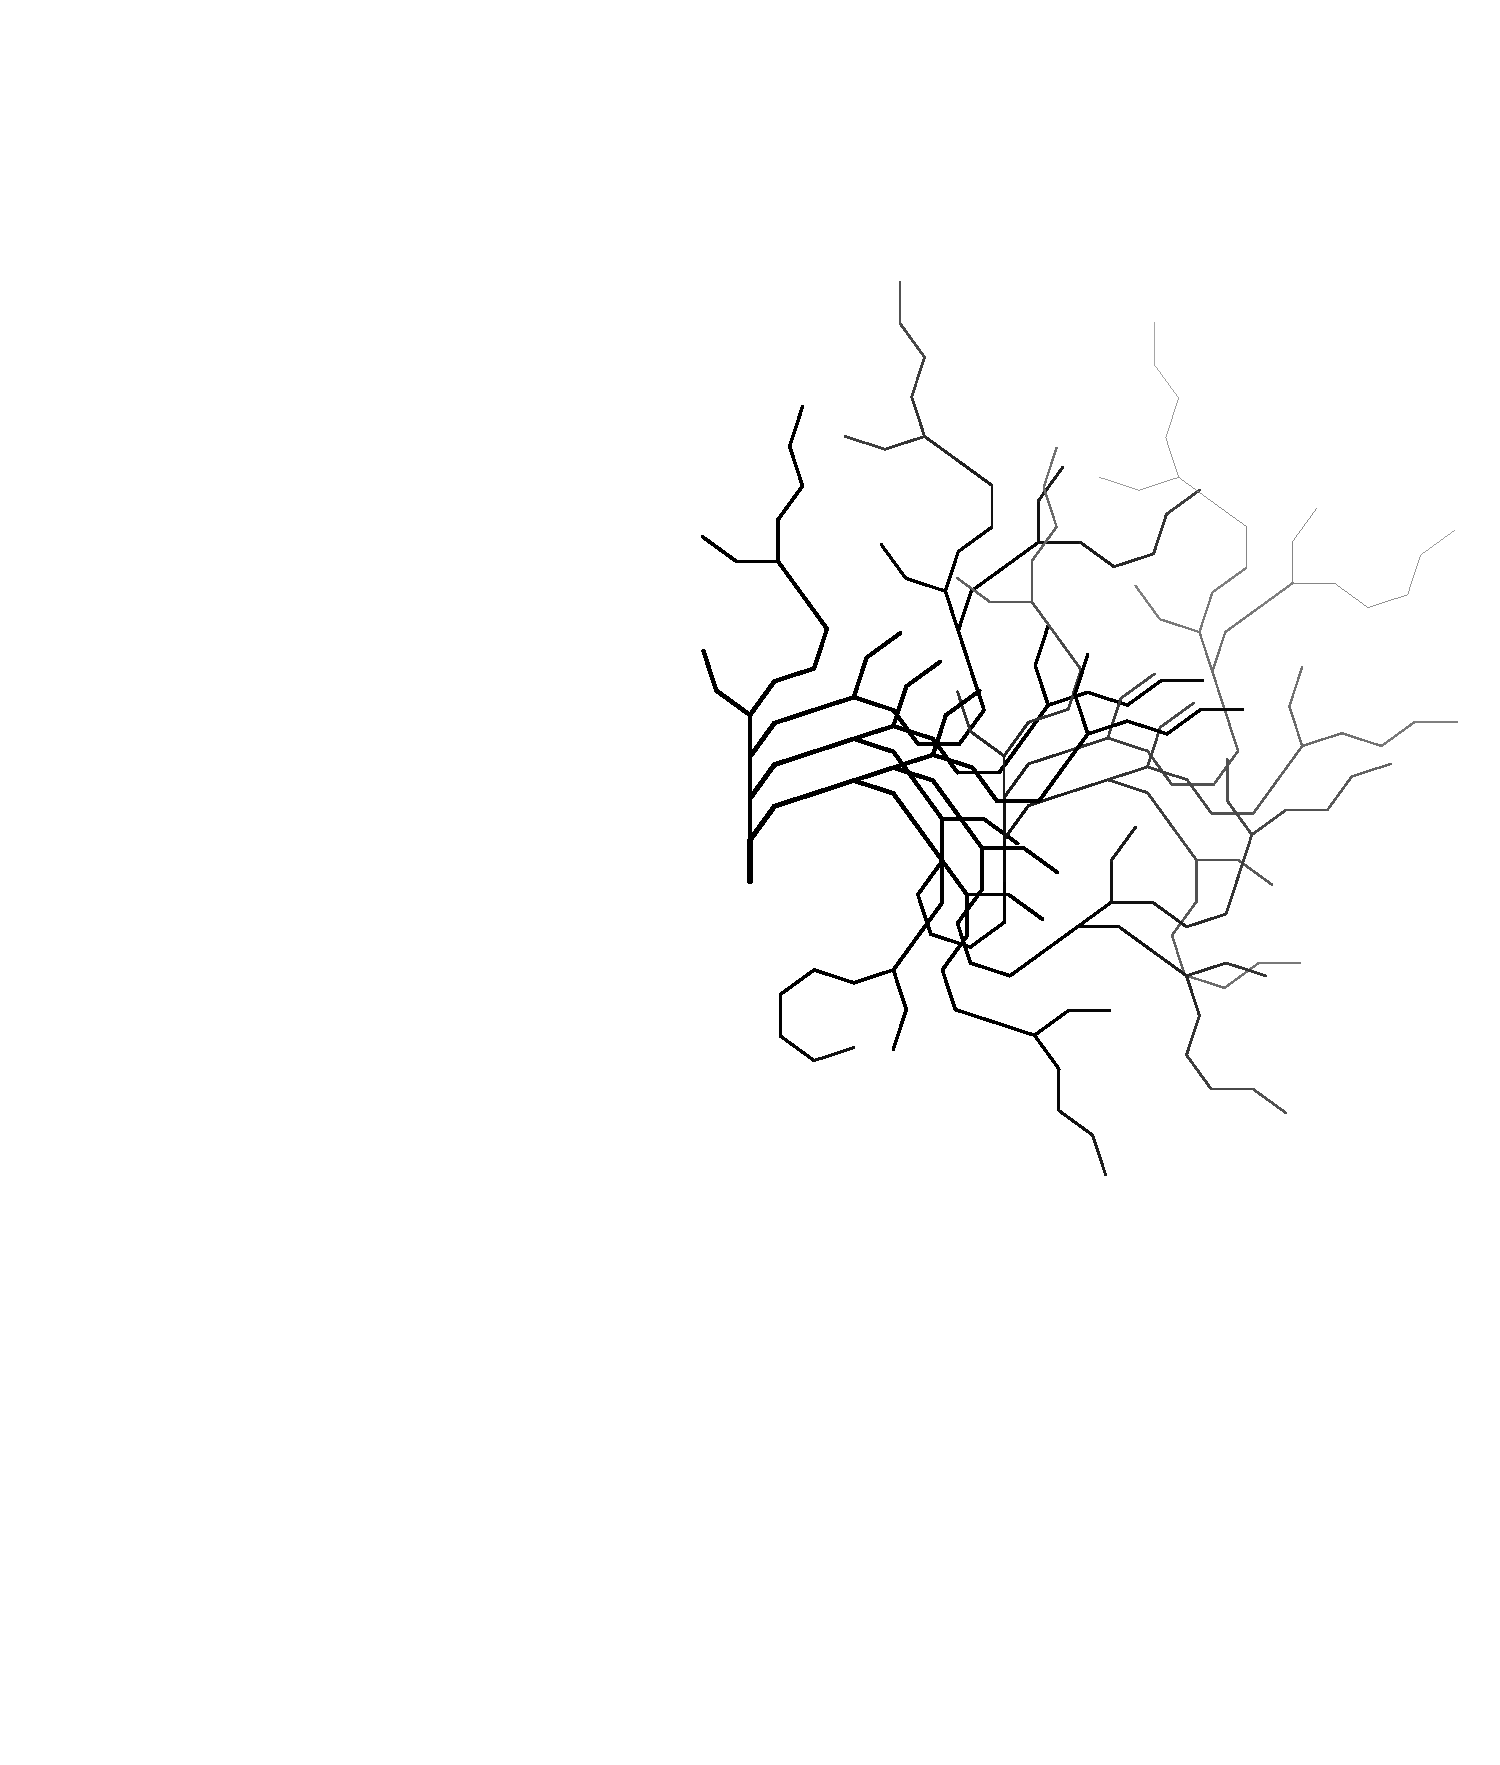
\includegraphics[clip=true, viewport=4in 3.5in 10in 10in, scale = 0.5]{Images/ThePathWeWillFollow4A}
		\caption[Mirror Left]{Mirror Left\footnotemark}
		\label {MirrorLeft}
	\end{subfigure}
	\begin{subfigure}{0.5\textwidth}
		\centering
		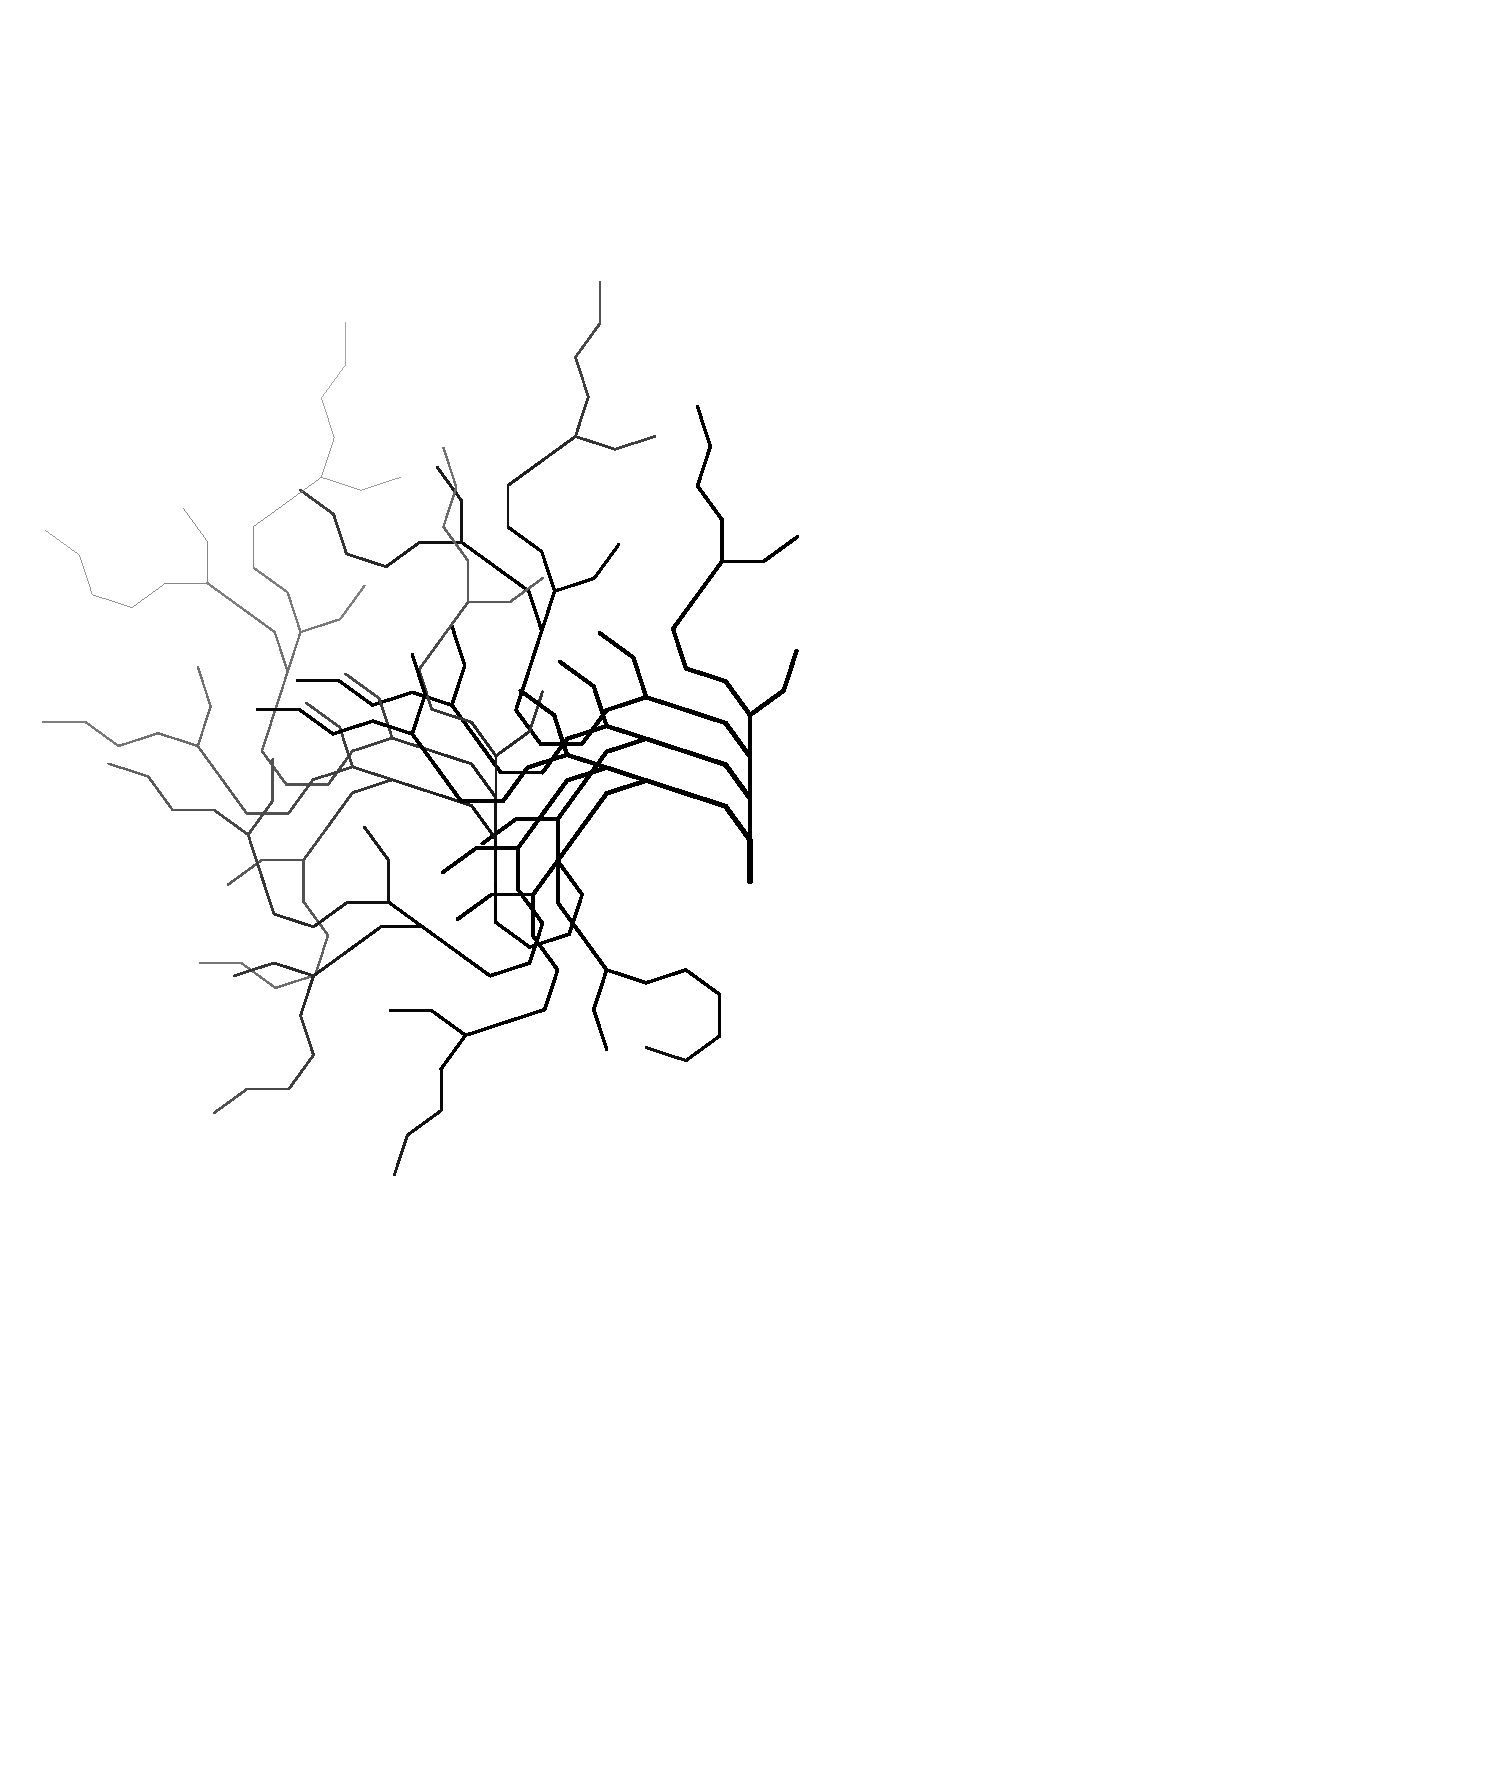
\includegraphics[clip=true, viewport=0in 3.5in 6in 10in, scale = 0.5]{Images/ThePathWeWillFollow4B}
		\caption[Mirror Right]{Mirror Right\footnotemark}	
		\label {MirrorRight}
	\end{subfigure}
	\caption[Mirrored L-Systems]{Mirrored L-Systems}
	\label{Same}
	\end{figure}
	
	\addtocounter{footnote}{-1}\footnotetext{A; A $\rightarrow$ F[A+FA–F]–F–FA+F; $\theta$ = 36$^{\circ}$, $\phi$ = 18$^{\circ}$; Iterations = 4; IW = 2, WC = 0.95}
	\addtocounter{footnote}{1}\footnotetext{A; A $\rightarrow$ F[A+FA–F]–F–FA+F; $\theta$ = -36$^{\circ}$, $\phi$ = -18$^{\circ}$; Iterations = 4; IW = 2, WC = 0.95}

	
	%\textcolor{blue}{[Two L-Systems on the left and right, facing each other]}

	
	
\chapter{What is an L-System?}

This is an L-System:

%\textcolor{blue}{[Picture of impressive looking L-system]}
	\begin{figure}[h]
	\centering
	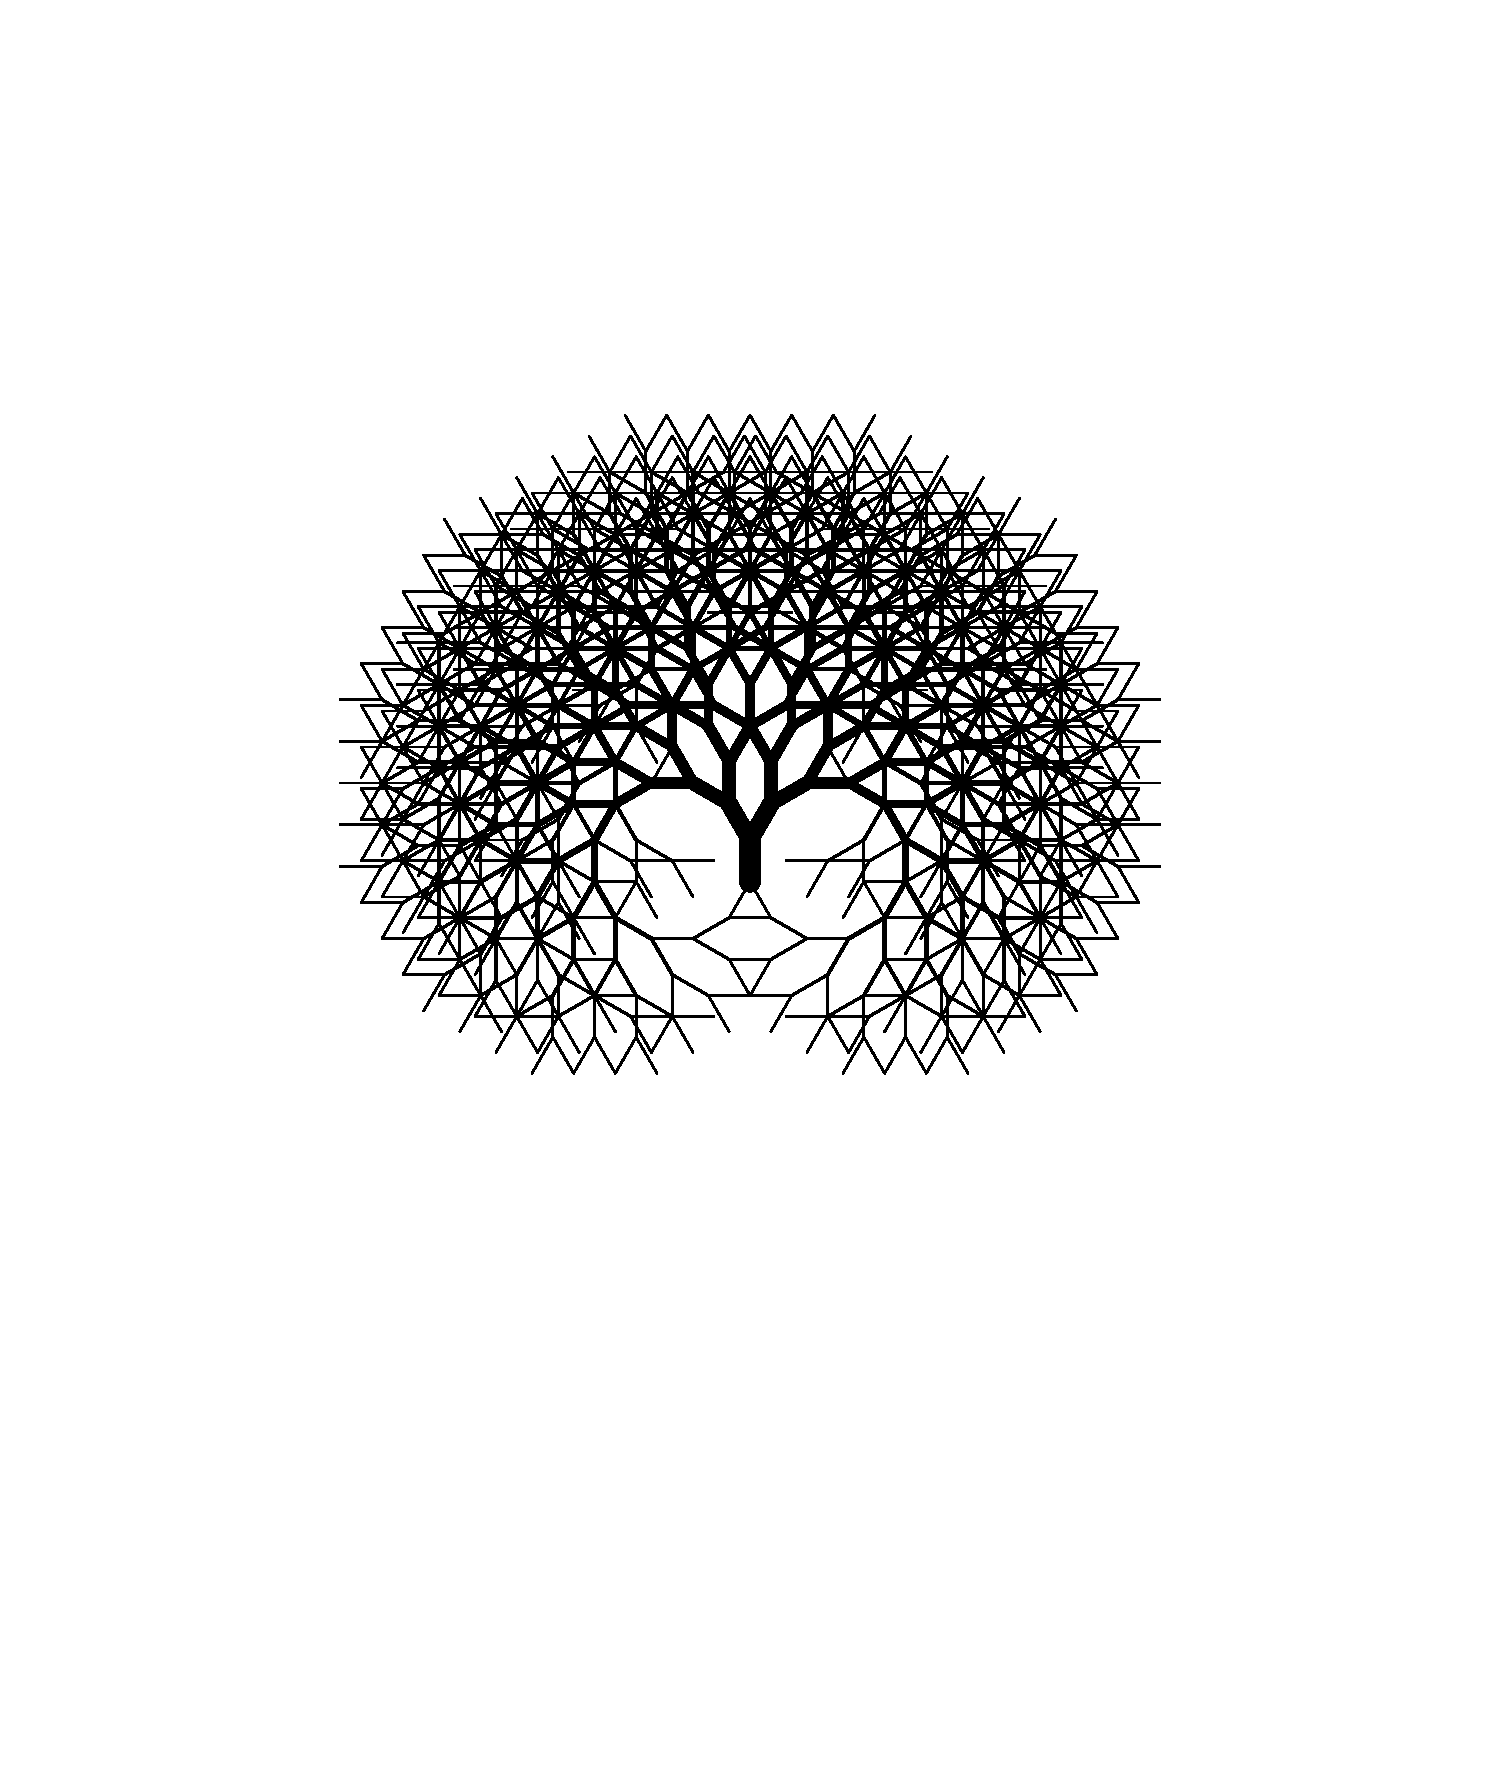
\includegraphics[clip=true, viewport=1in 4.6in 9in 9in, scale=0.45]{Images/WhatisanL-System1}
	\caption[Magnificent Tree]{Magnificent Tree\footnotemark}
	\label {Motivations3}
	\end{figure}
	\footnotetext{A; A $\rightarrow$ F[+A]–A; $\theta$ = 30$^{\circ}$; Iterations = 12}

	Well, it would be more right to say that this is the \textit{output} of an L-System. L-Systems are a \textit{technique} with which one can describe a complex, changing system with a few letters and symbols. This chapter will cover a few main ideas. The first, and most central, is a discussion of the mechanics of how they work, how to interpret them, and how to create them. I’ll illustrate particularly effective ways these systems can be used, how I’ve used them, (including some early experimentations before the central project,) and end with a lead-in to the central coding portion of this thesis, the L-Systems Explorer.

	There are a few effective ways I've found to introduce L-Systems to people. I'll go through each of these different strategies to give you some solid footing before we really dig into the material.


\section{Understanding through Definitions}
\label{Understanding-through-Definitions}

	Before I describe the structure of an L-System, I'd like to introduce you to the idea of a \textit{string}. A \textit{string} in Computer Science is a more expansive way of saying a \textit{word}. A string does not need to be in any dictionary, however, and it can include essentially any character that can be written on a computer. This includes numbers, symbols like \code{\&}, \code{\%}, and \code{+}, as well as some other special characters. When I say ``string", I mean a word that consists of some combination of these characters, for example: \code{DFS\&2*|:09} or \code{!!n./?;}. Strings do not need to be able to be spoken aloud to be valid. A string can also be ``empty", meaning that it contains no characters, though it is still a string. They may also be only one character long.
	
	L-Systems have four essential parts. The first part is the \code{start} variable. It is usually just a character, we'll call it \code{A} here. This will be the initial value of the structure, something akin to a ``seed". The second part is a set of rules that describe how the L-System grows (which is explained more in the next paragraph). These rules are usually written like \code{A} $\rightarrow$ \code{AB} or \code{B} $\rightarrow$ \code{AA}, where each of these is a different rule. In this thesis, I will call \code{A}, \code{B}, and other values with rules, ``productions". Similarly, each of these rules is called a ``production rule". The third part of an L-System is the angle or angles that it uses to change its state. Some of the L-Systems I show in this thesis use a second angle $\phi$ in addition to the required $\theta$. This $\phi$ establishes a baseline difference for values that use $\theta$ so that an L-System isn't just reduced to a line when $\theta$ = 0. The fourth part is the \code{Iterations}, which is the number of times the production rules are applied to a string. Some L-Systems I made for this thesis use an entirely optional fifth part, which has two values and governs the width of the lines. Initial Width (IW) is the pixel width of the first line. Width Change (WC) is the multiplier applied to the line width of each successive line. Unless otherwise stated, the value for $\phi$ is 0 and the value for both IW and WC is 1.
	
	%\textcolor{blue}{[(filler?) L-System that looks like a word]}
	\begin{figure}[h!]
	\centering
	
\includegraphics[clip=true, viewport=4in 5.68in 7in 6.37in, scale=1]{Images/UnderstandingThroughDefinitions1}
	\caption[Almost an Octagon]{Almost an Octagon\footnotemark}
	\label {UnderstandingThroughDefinitions1}
	\end{figure}
	\footnotetext{A; A $\rightarrow$ F+A; $\theta$ = -45$^{\circ}$; Iterations = 7}
	
	To draw an image from an L-System, we follow a set of carefully stated instructions. First, we save the start variable as a special string, we'll call it the L-string. If the start variable was \code{A}, then the L-string is also \code{A}. Then, we repeat a specific step some number of times determined by the value of \code{Iterations}. If \code{Iterations} is 5, then we will repeat the following step 5 times:\\
	
	\begin{addmargin}[4em]{4em}
	- For every character in the L-string, if that character has an associated production rule, then that character is replaced in the L-string by its production rule. (For example, if the L-string is \code{A}, and there is a production rule \code{A} $\rightarrow$ \code{BA}, then the new L-string after this step is \code{BA}.) If that character does not have a specified production rule, then it is implied that its production rule consists of itself.\\
	 \end{addmargin}
	 
	 With this simple step as a guideline, we can construct even the most complicated L-Systems. It might seem strange that this one rule is capable of such complexity, but that surprise is the mood that I'm encouraging you to see as a fundamental feature of these structures. There may be more opportunities to be surprised!

	%\textcolor{blue}{[Some extremely simple L-Systems]}
	\begin{figure}[h!]
	\centering
	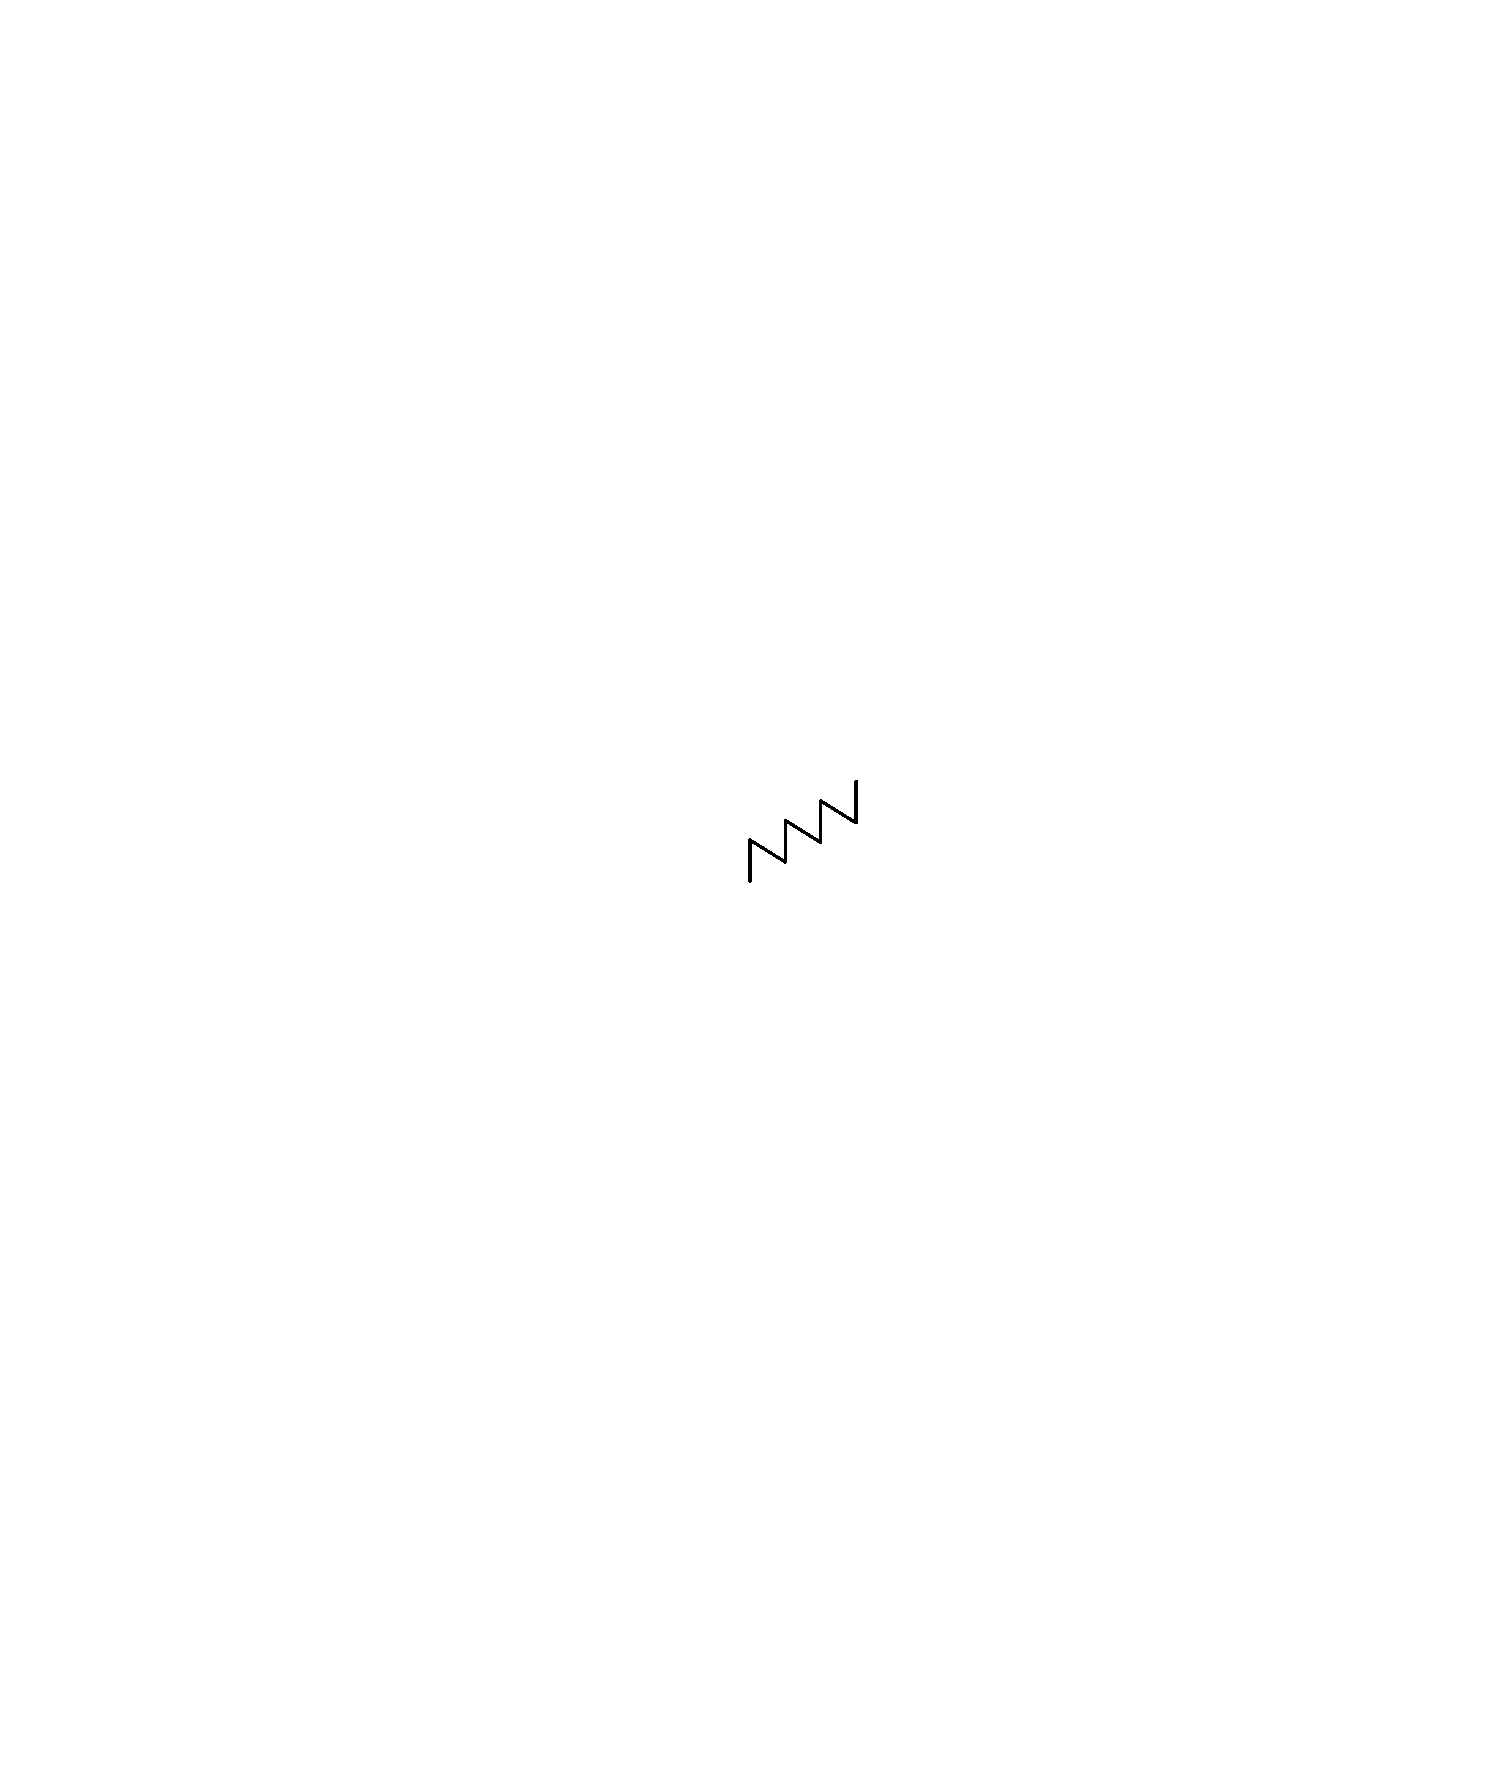
\includegraphics[clip=true, viewport=4in 5.8in 7in 6.5in, scale=1]{Images/UnderstandingThroughDefinitions2}
	\caption[A Simple Squiggle]{A Simple Squiggle\footnotemark}
	\label {UnderstandingThroughDefinitions1}
	\end{figure}
	\footnotetext{A; A $\rightarrow$ F+B, B $\rightarrow$ F–A; $\theta$ = -122$^{\circ}$; Iterations = 7}
	%L-Systems are what we in CS would call a \textit{Recursive Replacement structure}. This describes the way in which an L-System makes more of itself. 
	
	While these images are intended to help describe the process of building an L-System, keep in mind that they are ultimately just \textit{visualizations}. The L-Systems are only the \textit{strings}. Thinking that L-Systems are the images might not be entirely accurate, but I admit that the image and the string are so closely tied that the distinction isn't all that important. Yet still, there \textit{is} a difference.

\section{Understanding through Images}
\label{Understanding-through-Images}

	L-Systems can be slippery if there's no visual output to latch onto. I think that one of the best ways to engage with these structures is through connecting the images with the strings that describe them. One can see that everything in the image has an origin in the string, and that there is nothing lost between the image and the string. No information is lost. I suggest alternative visualization strategies in Section \ref{Interpretations}.
	
	Figure \ref{Simple1} shows the appearance of an L-System as the number of iterations increases from 0 to 3. There is a sense that the L-System is ``growing" here, fittingly tied to their origin as plant-modeling software. The text below each set of images is the L-string that constructed those images.

	The info of this L-System: ``start: A; rules: A $\rightarrow$ –FB, B $\rightarrow$ +FA; $\theta$: 45$^{\circ}$".

%\textcolor{blue}{[Image A0]}: \code{Iterations = 0, current string: A}\\
%\textcolor{blue}{[Image A1]}: \code{Iterations = 1, current string: -FB}\\
%\textcolor{blue}{[Image A2]}: \code{Iterations = 2, current string: -F+FA}\\
%\textcolor{blue}{[Image A3]}: \code{Iterations = 3, current string: -F+F-FB} \\

	\begin{figure}[H]
	\begin{subfigure}{0.25\textwidth}
		\centering
		
\includegraphics[height=0.8\textwidth]{Images/A0}
		\caption{A}
		\label {A0}
	\end{subfigure}%
	\begin{subfigure}{0.25\textwidth}
		\centering
		
\includegraphics[height=0.8\textwidth]{Images/A1}
		\caption{–FB}
		\label {A1}
	\end{subfigure}%
	\begin{subfigure}{0.25\textwidth}
		\centering
		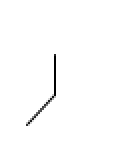
\includegraphics[height=0.8\textwidth]{Images/A2}
		\caption{–F+FA}
		\label {A2}
	\end{subfigure}%
	\begin{subfigure}{0.25\textwidth}
		\centering
		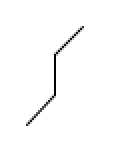
\includegraphics[height=0.8\textwidth]{Images/A3}
		\caption{–F+F–FB}
		\label {A3}
	\end{subfigure}
	\caption{First Simple L-System}
	\label{Simple1}
	\end{figure}



	Figure \ref{Simple2} uses the same start variable and angle, but different production rules. Each image still displays the appearance of the L-System as the number of iterations goes from 0 to 3. 

	The info for this L-System: ``start: A; rules: A $\rightarrow$ F–B, B $\rightarrow$ F+A; $\theta$: 45$^{\circ}$".

%\textcolor{blue}{[Image B0]}: \code{Iterations = 0, current string: A}\\
%\textcolor{blue}{[Image B1]}: \code{Iterations = 1, current string: F-B}\\
%\textcolor{blue}{[Image B2]}: \code{Iterations = 2, current string: F-F+A}\\
%\textcolor{blue}{[Image B3]}: \code{Iterations = 3, current string: F-F+F-B} \\

	\begin{figure}[h]
	\begin{subfigure}{0.25\textwidth}
		\centering
		
\includegraphics[height=0.8\textwidth]{Images/B0}
		\caption{A}
		\label {B0}
	\end{subfigure}%
	\begin{subfigure}{0.25\textwidth}
		\centering
		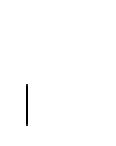
\includegraphics[height=0.8\textwidth]{Images/B1}
		\caption{F–B}
		\label {B1}
	\end{subfigure}%
	\begin{subfigure}{0.25\textwidth}
		\centering
		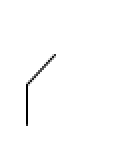
\includegraphics[height=0.8\textwidth]{Images/B2}
		\caption{F–F+A}
		\label {B2}
	\end{subfigure}%
	\begin{subfigure}{0.25\textwidth}
		\centering
		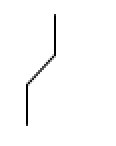
\includegraphics[height=0.8\textwidth]{Images/B3}
		\caption{F–F+F–B}
		\label {B3}
	\end{subfigure}
	\caption{Second Simple L-System}
	\label{Simple2}
	\end{figure}

 Look at the L-System in Figure \ref{HexUnderstanding} and see how the different productions can be seen in the output. (The long straight sections are generated by \code{A} and the branch joints come from \code{B}.) The starting point is the open-ended branch in the middle of the image.

	%\textcolor{blue}{[L-System with the multiple very different production rules, and the effects of each production node can be clearly seen in the output]}
	\begin{figure}[H]
	\centering
	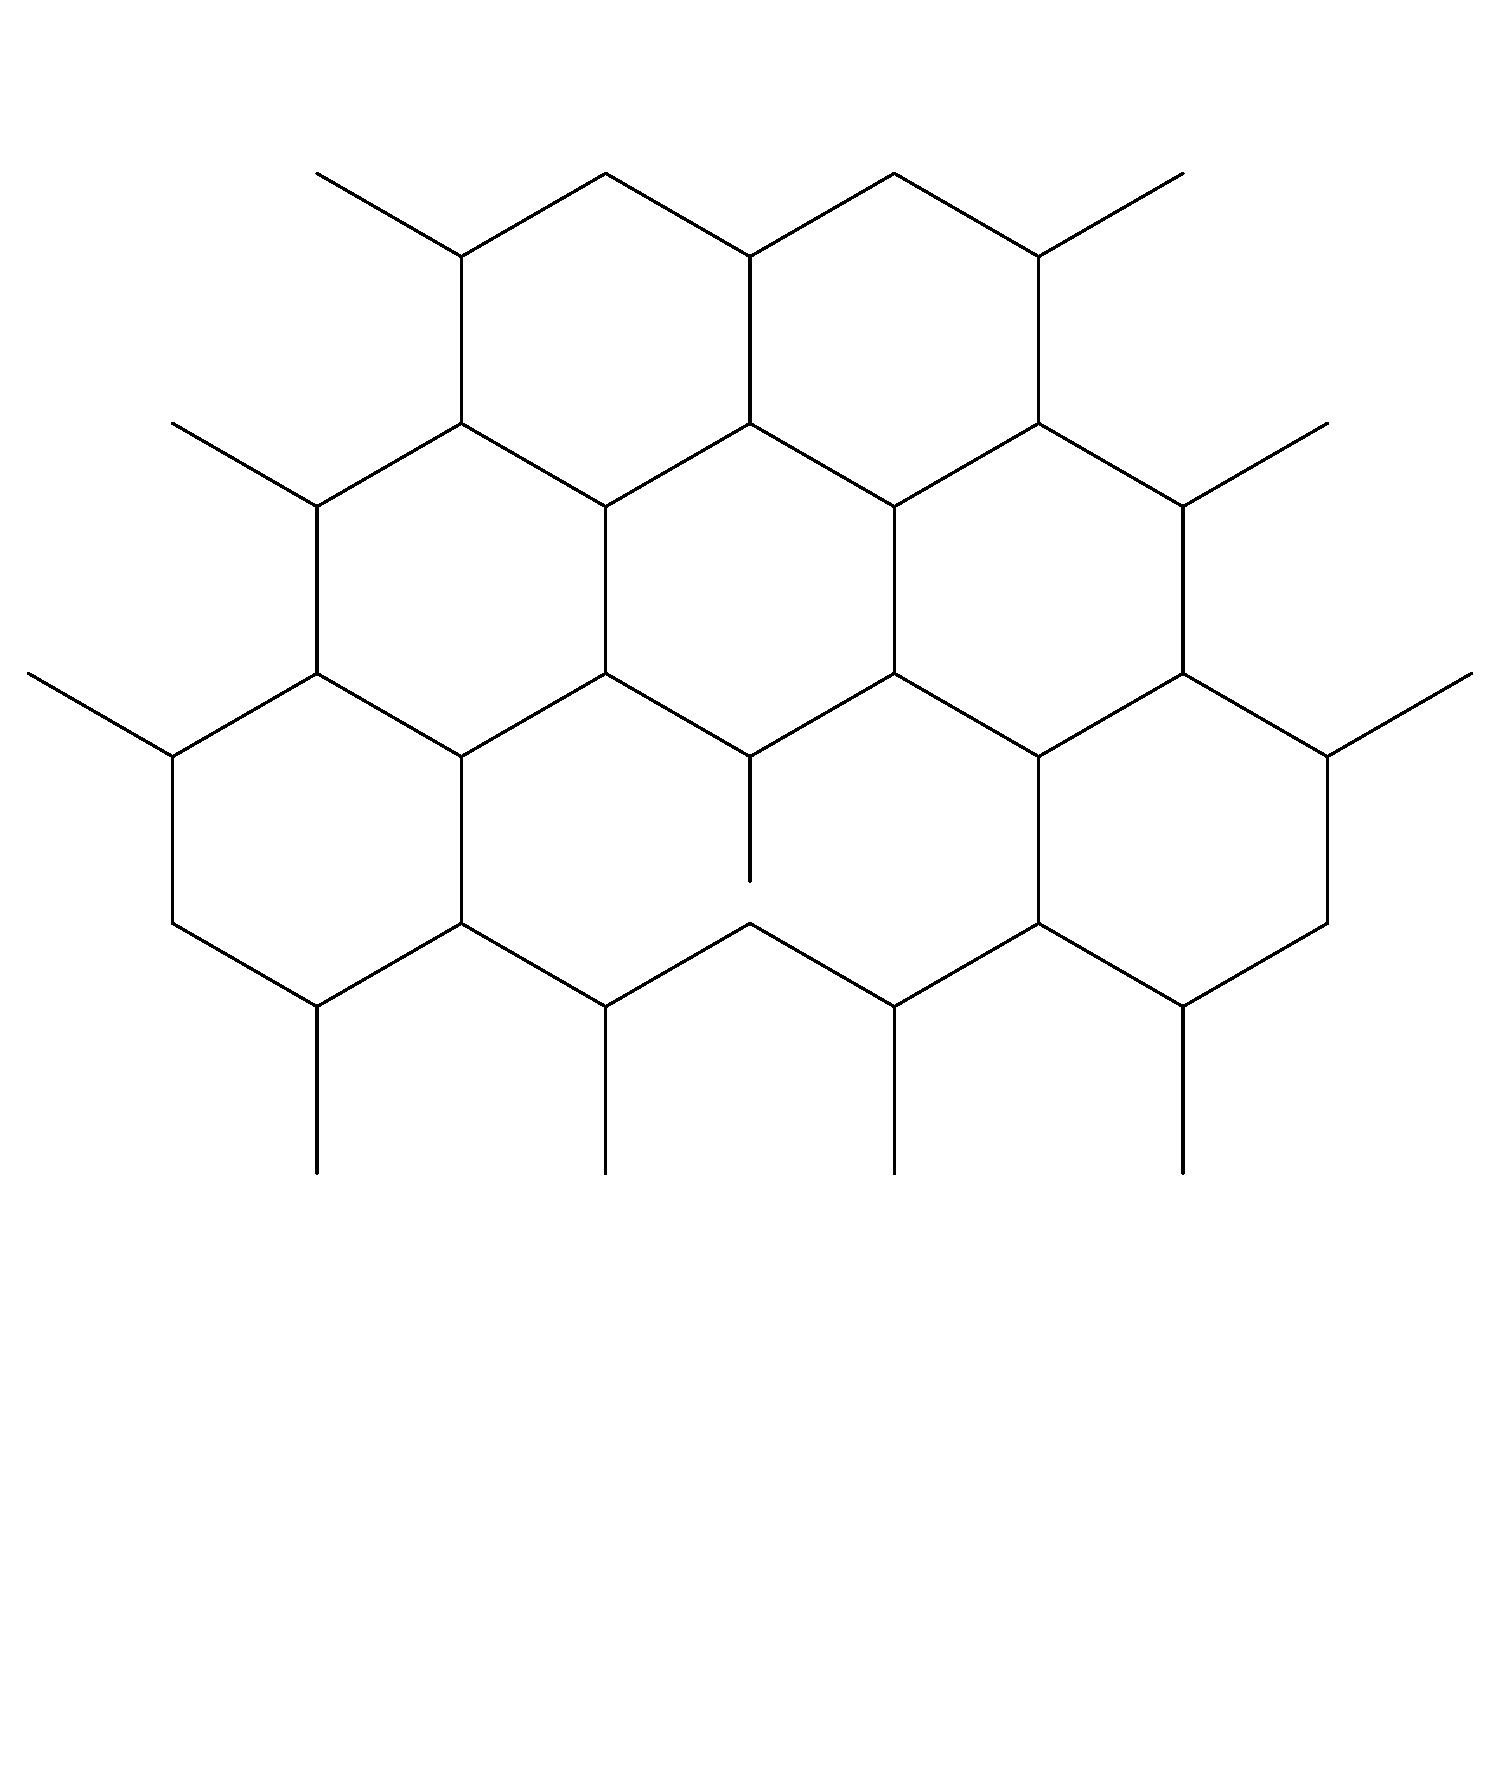
\includegraphics[clip=true, viewport=0in 4in 10in 11in, scale=0.5]{Images/UnderstandingThroughImages2}
	\caption[Distinct Productions]{Distinct Productions\footnotemark}
	\label {HexUnderstanding}
	\end{figure}
	\footnotetext{A; A $\rightarrow$ FFFB, B $\rightarrow$ +[– –FA]FA; $\theta$ = 60$^{\circ}$; Iterations = 11}

\subsection{Turtle Graphics}
\label{Turtle-Graphics}

	%\textcolor{blue}{[An image of the turtle]}
	\begin{figure}[H]
	\centering
	
\includegraphics[scale = 3]{Images/Turtle}
	\caption{The ``Turtle" used in Turtle Graphics}
	\label {Turtle}
	\end{figure}

	My early attempts to make L-System drawing programs all utilized a concept called ``Turtle Graphics". [cite Seymour paper "Mindstorms"] Turtle Graphics is a simple program that is often used in introductory Computer Science classes to help get students familiar with the basics of coding. It's used in \textit{The Algorithmic Beauty of Plants} to draw most of their L-Systems. I've also seen it used in other L-System implementations online. Turtle Graphics operates by reading a series of instructions and drawing according to those instructions. This is particularly applicable for L-Systems, where each symbol can be associated with a specific operation, such as drawing a straight line or turning to face in a different direction. Even while making my Explorer from the ground up, I've kept in mind the Turtle Graphics strategy.
	
	%\textcolor{blue}{[A few simple turtle programs]}
	\begin{figure}[h]
	\begin{subfigure}{0.5\textwidth}
		\centering
		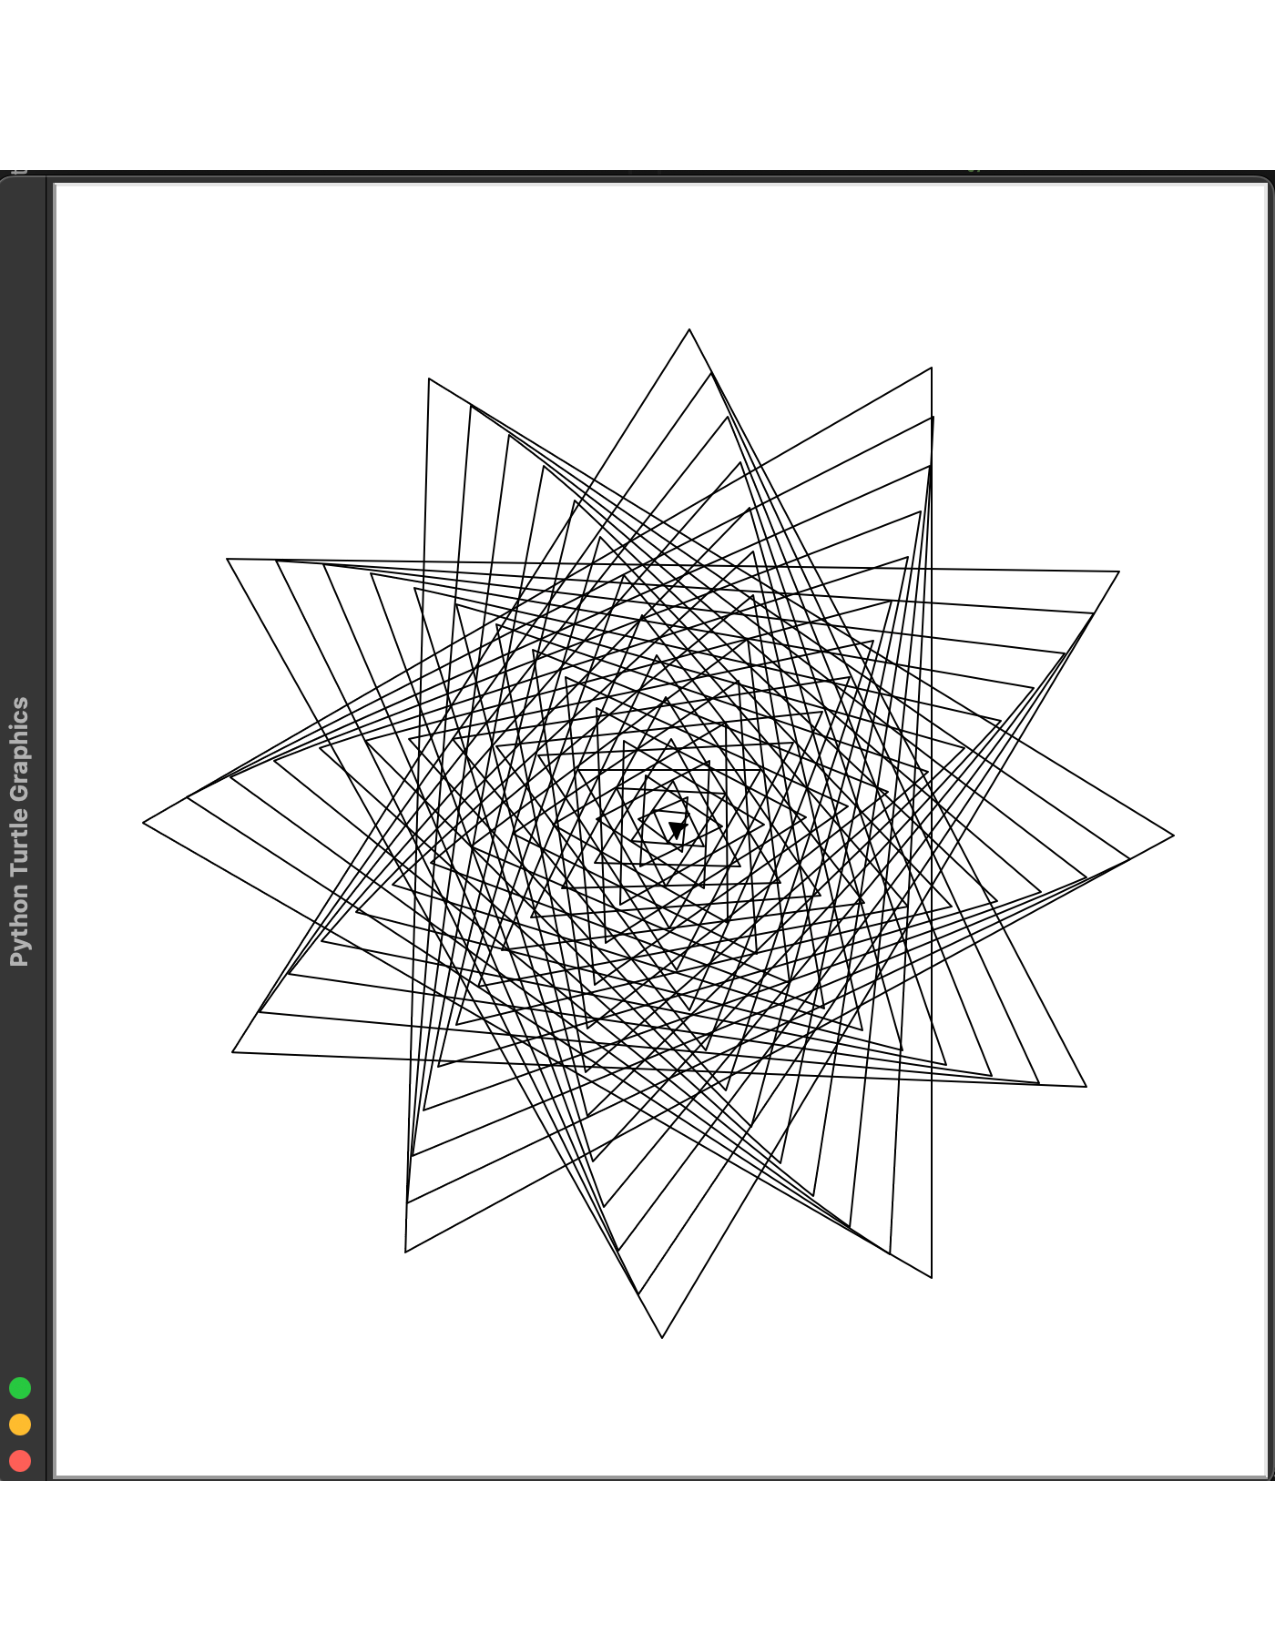
\includegraphics[clip=true, viewport=0.7in 2in 8in 9in, height = 0.7\textwidth]{Images/TurtleGraphics2}
		\caption{Simple Star}
		\label {TurtleGraphics2}
	\end{subfigure}%
	\begin{subfigure}{0.5\textwidth}
		\centering
		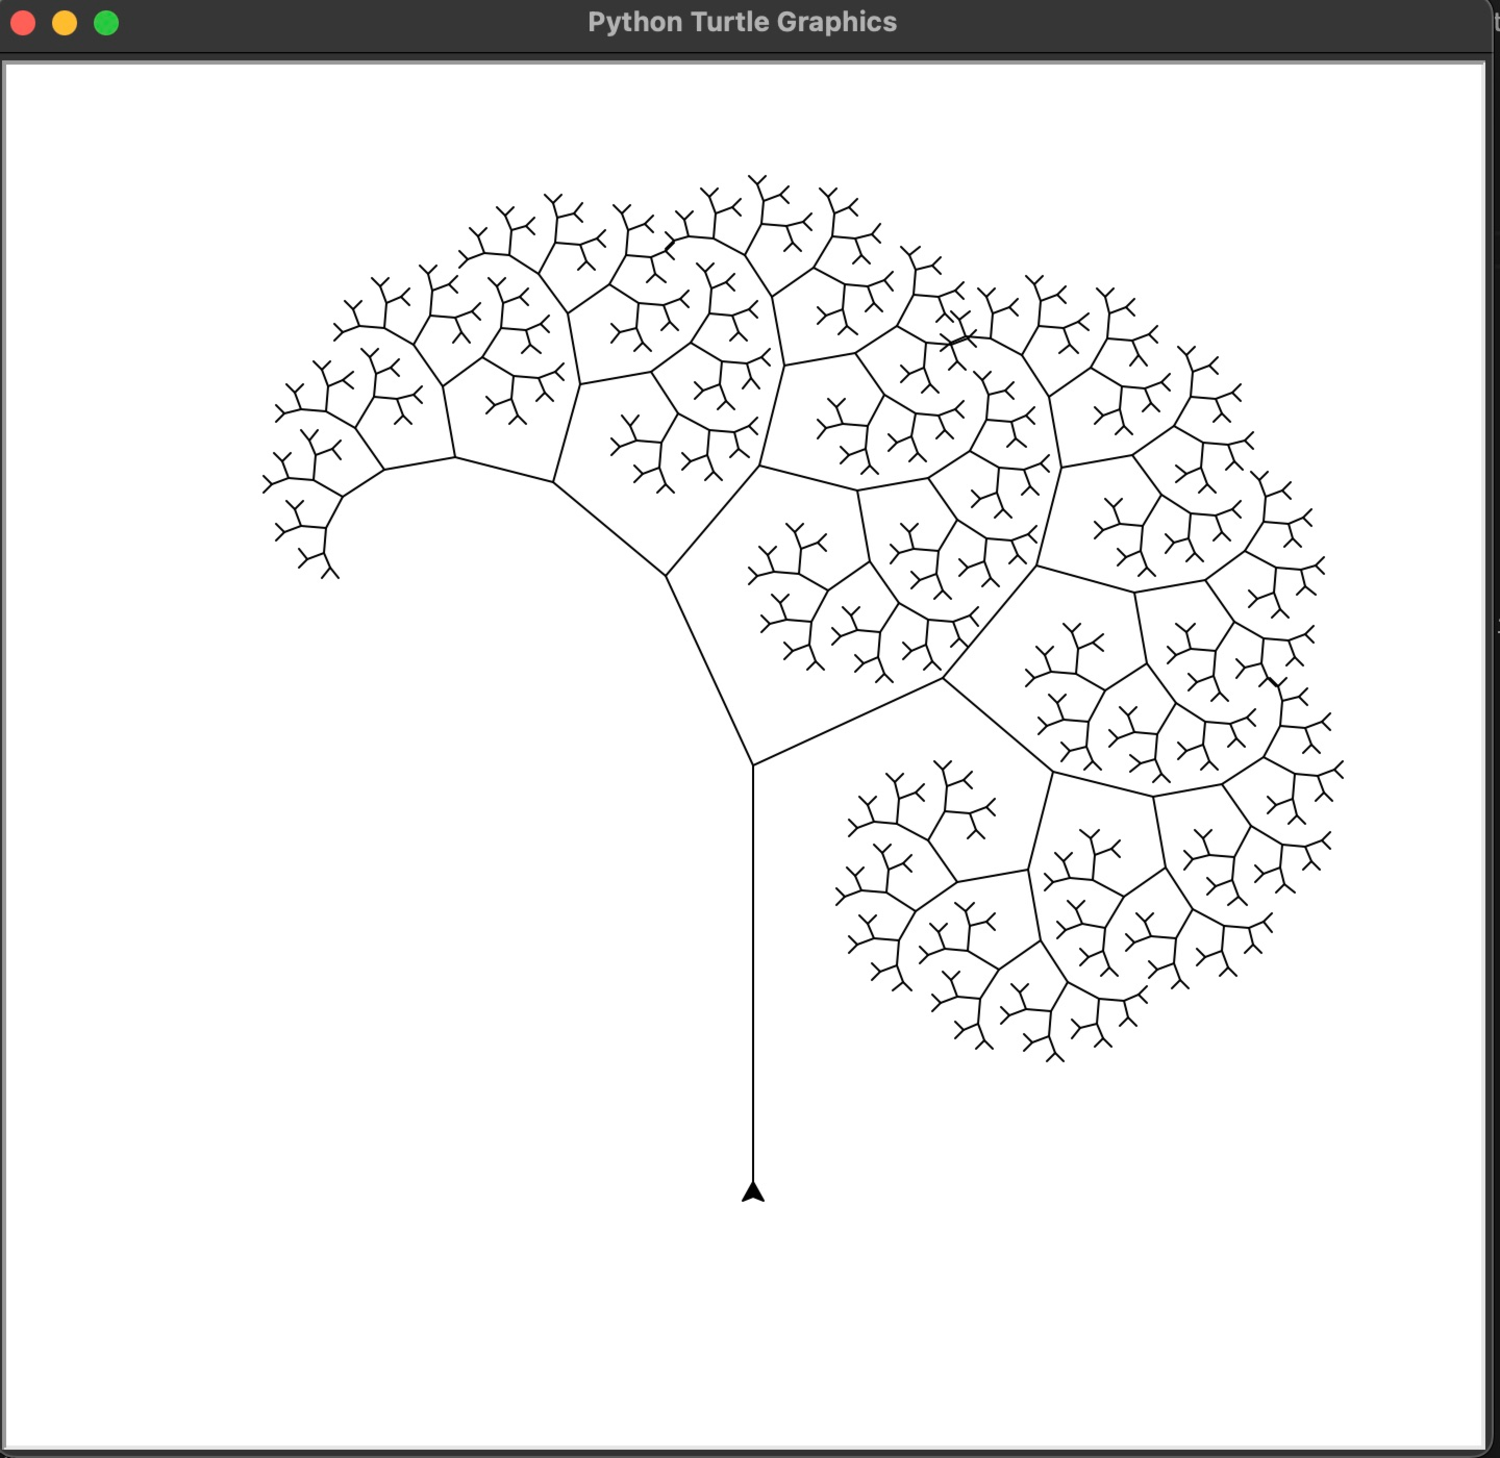
\includegraphics[clip=true, viewport=1.5in 1.3in 9.3in 8.7in, height = 0.7\textwidth]{Images/TurtleGraphics3}
		\caption{Fern}
		\label {TurtleGraphics3}
	\end{subfigure}
	\caption{Images generated with Turtle Graphics}
	\label{TurtleGraphics2and3}
	\end{figure}
	
	
	The central feature that Turtle Graphics uses to great effect is ``state". ``State" here means ``condition" or ``status". The ``Turtle" keeps track of its position and rotation. With an x-position, a y-position, and an angle, the Turtle is uniquely placed in its window. By manipulating these values with the code and choosing whether to draw or not draw between positions, the Turtle is able to seamlessly turn abstract code into clear visualizations. This is also particularly powerful because it physicalizes the process of coding that's often purely digital and accessible only through difficult-to-engage-with abstraction.
	
	Figure \ref{TurtleFractals} shows some fractals created with Turtle Graphics and L-Systems. Each of these could also be created with the L-System Explorer I introduce in the next chapter. L-Systems lend themselves particularly well to constructing fractals, due in part to their own recursive nature. 
	
	%\textcolor{blue}{[A variety of turtle-produced programs, some in color]}
	\begin{figure}[h]
	\begin{subfigure}{0.5\textwidth}
		\centering
		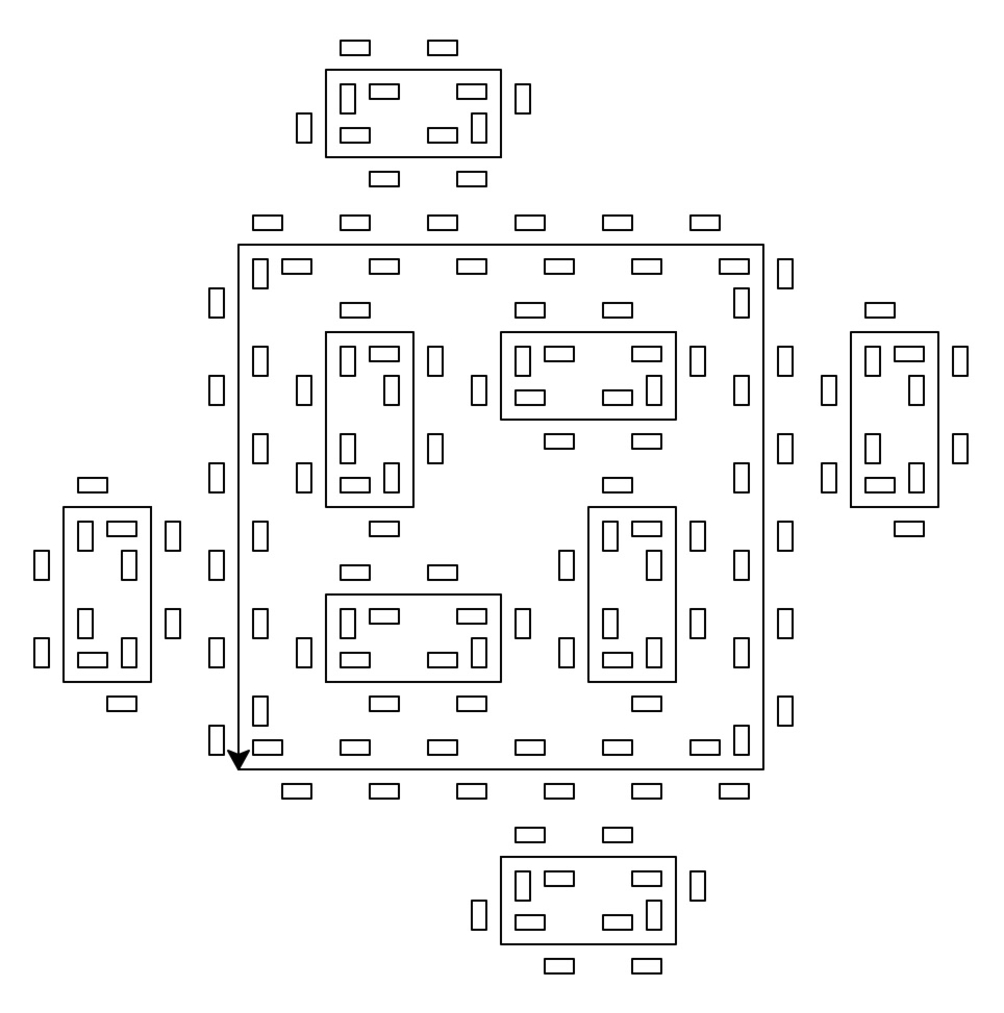
\includegraphics[height = 0.9\textwidth]{Images/TurtleGraphics4}
		\caption{Islands \& Lakes\footnotemark}
		\label {TurtleGraphics4}
	\end{subfigure}%
	\begin{subfigure}{0.5\textwidth}
		\centering
		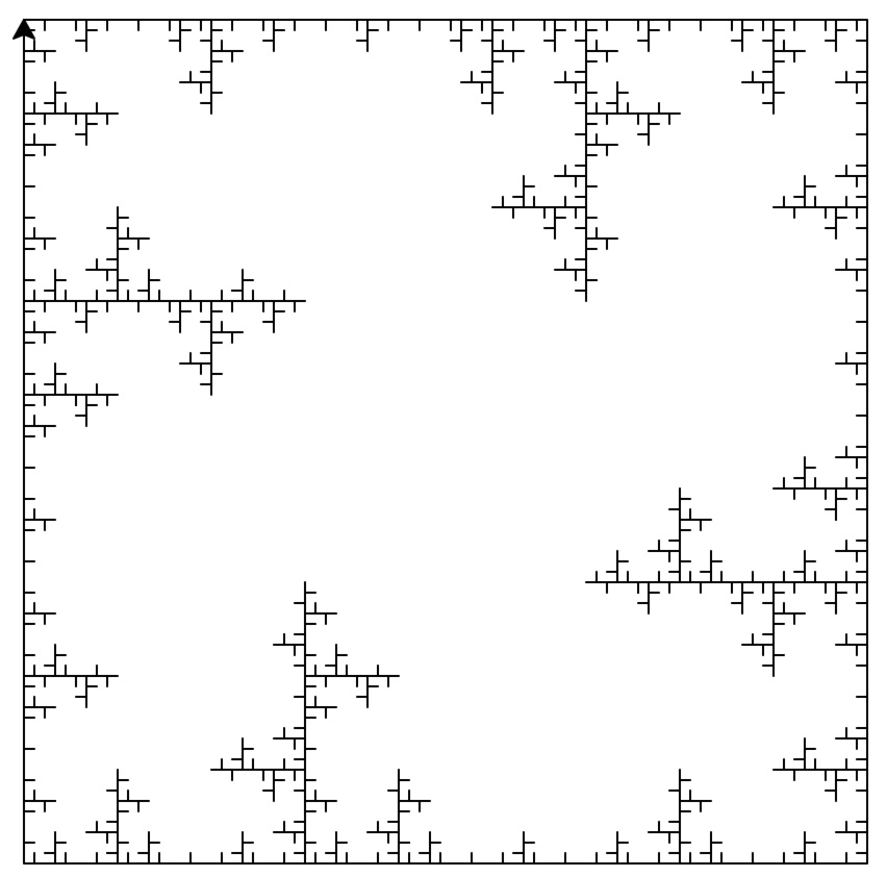
\includegraphics[height = 0.9\textwidth]{Images/TurtleGraphics5}
		\caption{Frame\footnotemark}
		\label {TurtleGraphics5}
	\end{subfigure}
	\centering
	\begin{subfigure}{0.5\textwidth}
		\centering
		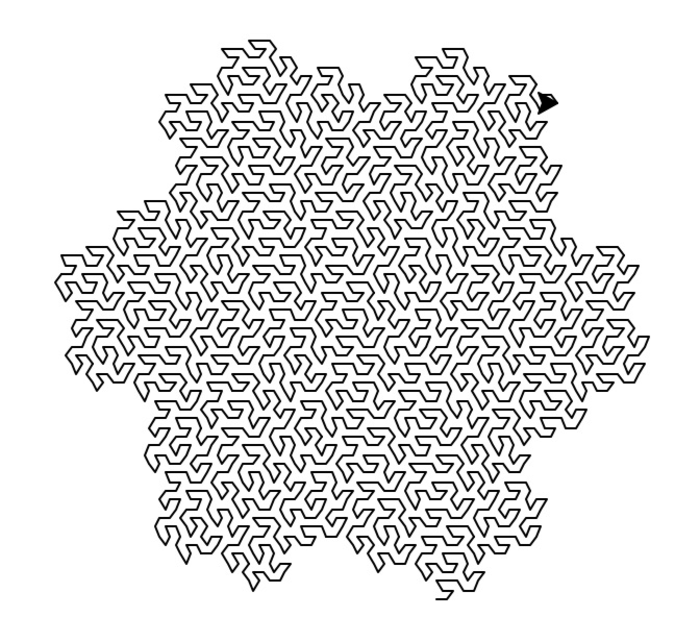
\includegraphics[height = 0.9\textwidth]{Images/TurtleGraphics6}
		\caption{Space-filling Hex\footnotemark}
		\label {TurtleGraphics6}
	\end{subfigure}
	
	\caption[L-Systems visualized with Turtle Graphics]{L-Systems visualized with Turtle Graphics\footnotemark}
	\label{TurtleFractals}
	\end{figure}
	
	\addtocounter{footnote}{-3}
	\footnotetext{F–F–F–F; F $\rightarrow$ F+f–FF+F+FF+Ff+FF–f+FF–F–FF–Ff–FFF, f $\rightarrow$ ffffff; $\theta$ = 90; Iterations = 2}
	\addtocounter{footnote}{1}
	\footnotetext{F–F–F–F; F $\rightarrow$ FF–F– –F–F; $\theta$ = 90; Iterations = 4}
	\addtocounter{footnote}{1}
	\footnotetext{F$_L$; F$_L$ $\rightarrow$ F$_L$+F$_R$++F$_R$–F$_L$– –F$_L$F$_L$–F$_R$+, F$_R$ $\rightarrow$ –F$_L$+F$_R$F$_R$++F$_R$+F$_L$– –F$_L$–F$_R$; $\theta$ = 60; Iterations = 4}
	\addtocounter{footnote}{1}
	\footnotetext{The L-strings for these images were given in ABOP (\cite{ABOP1990})}

\chapter{The L-Systems Explorer}

	In order to share my understanding about and my excitement for L-Systems, I wrote a program that allows users to interactively and graphically edit L-Systems and immediately see them visualized. My goal was to create a program that would reduce the barrier to entry of understanding these systems. My first explorations into making this space more accessible were done through turtle implementations in a basic Python program and later in a Blender program.\footnote{\cite{Blender2018}} I'll talk about these in more detail later in the thesis. Both of these strategies still heavily relied on the user to type input. It might as well have been code. It became clear that if I was to create something that was as accessible as I wanted that it to be, I would have to change my approach. In conversation with my advisor and through resources online for projects like mine, I found \textit{Processing}.\footnote{\cite{processing2014}}
	
		
	\begin{figure}[h!]
	\centering
	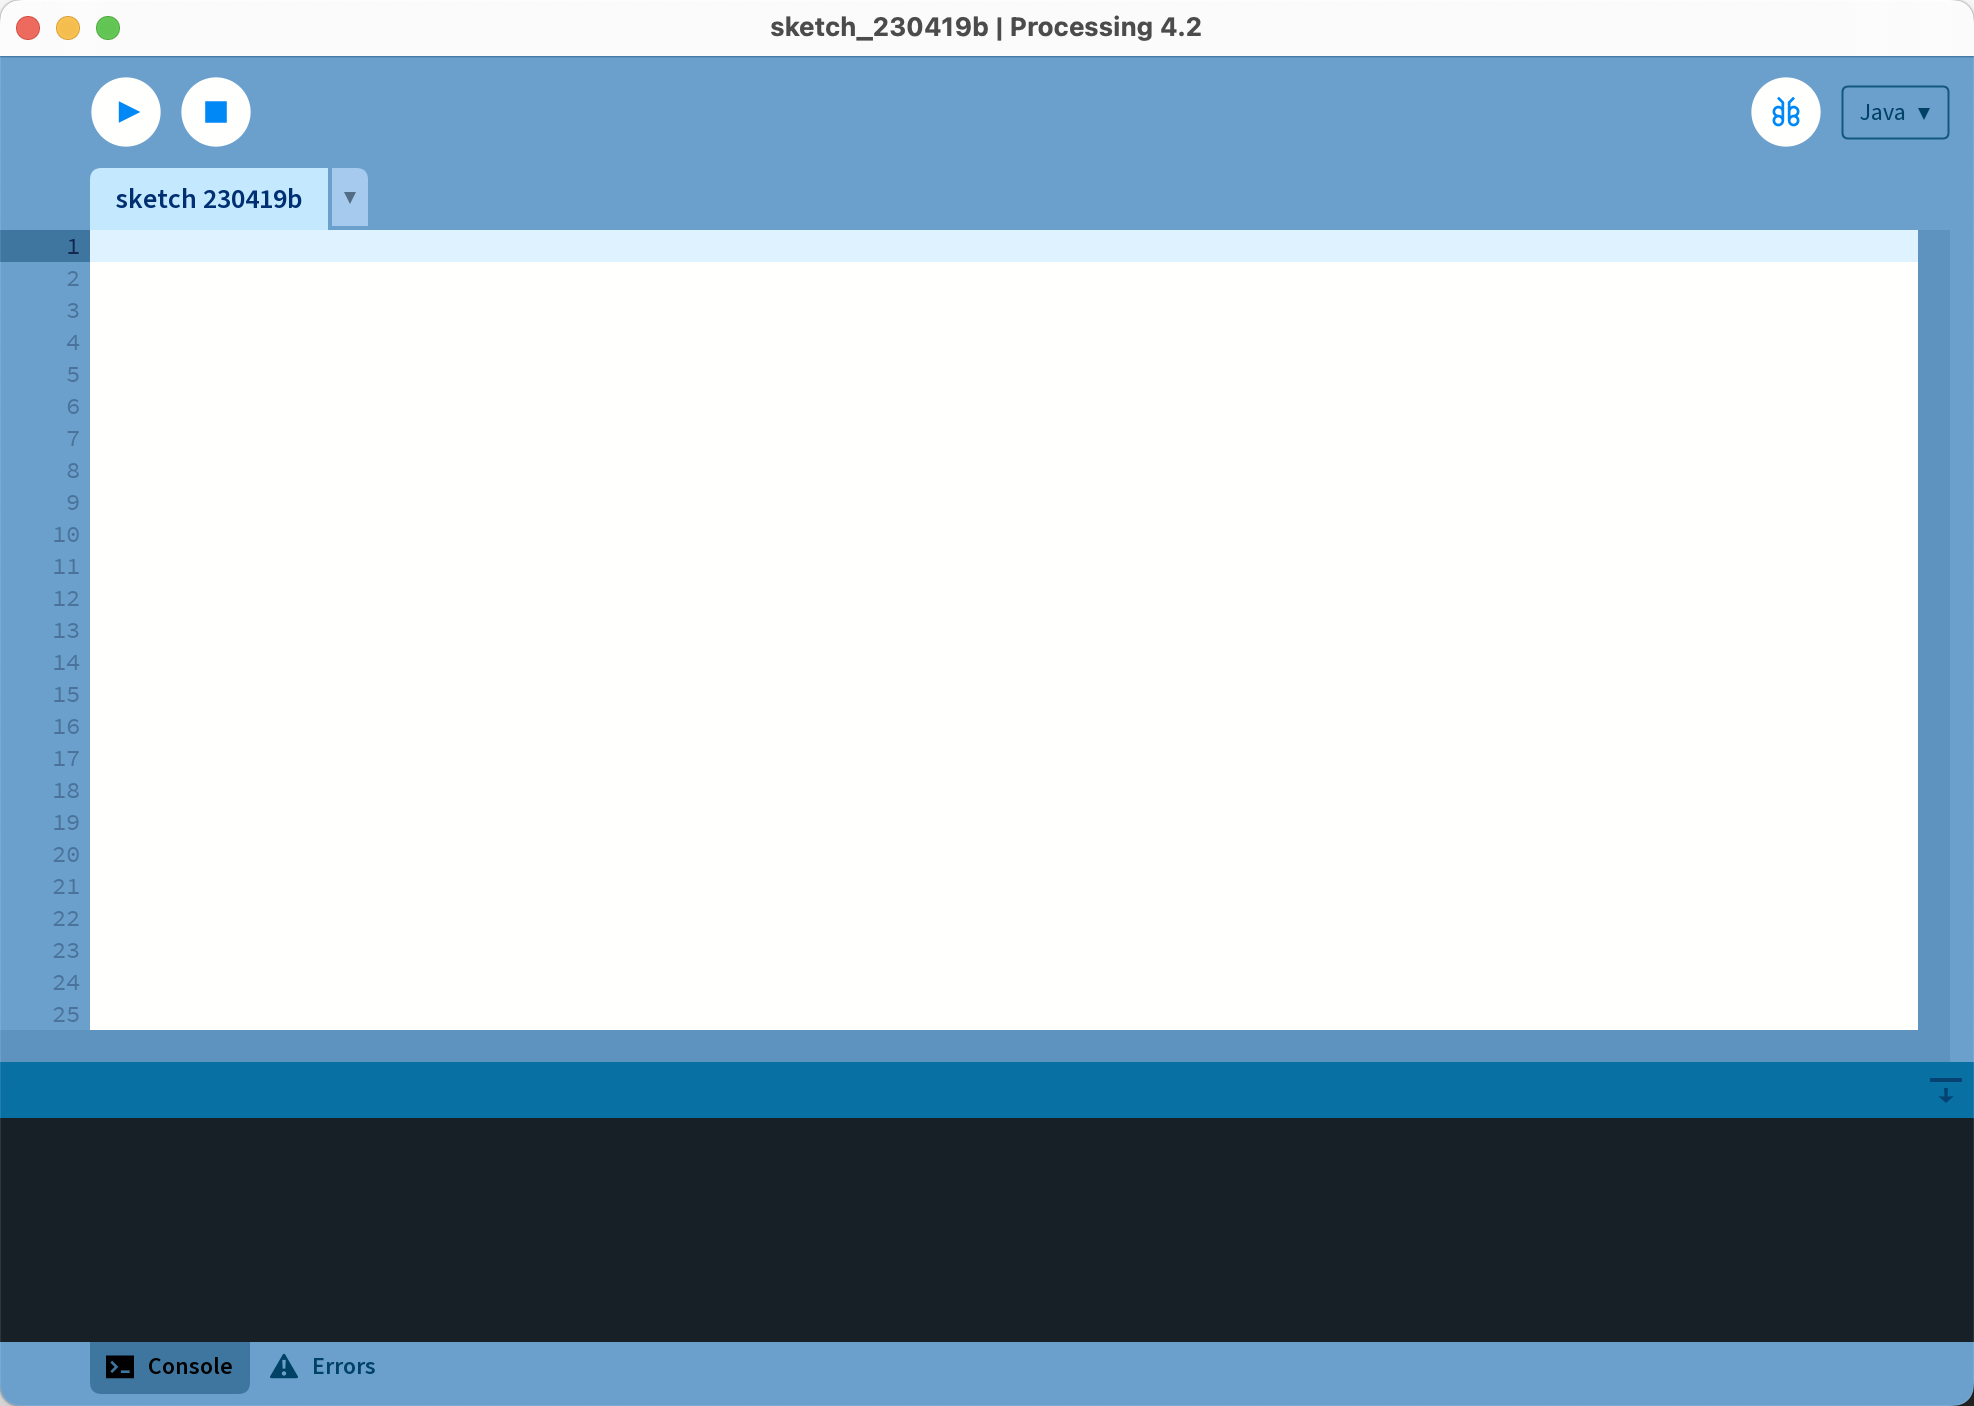
\includegraphics[scale=0.3]{Images/ProcessingWindow}
	\caption{A blank Processing window}
	\label {ProcessingWindow}
	\end{figure}
	
\section{What is \textit{Processing}?}

	%\textcolor{blue}{[A blank Processing window]}


	\textit{Processing} is a programming language and development environment written in Java and optimized for image generation. It was released by Casey Reas and Ben Fry in 2001 and has since found popular use as an art and educational tool. I chose to work with Processing because it was easy to use and appealed to my sensibilities as it is an open-source, free software. It also engages with the act of coding in the same way that artists have traditionally engaged with their mediums, which I also appreciated. In other programming languages, it often takes some time to go beyond just printing \code{hello world}. The first programs that people write in Processing produce concrete objects that can interact with the user, like a square that changes color when you hover over it. In Processing, coding \textit{is} art.
	
	To download and experiment with Processing yourself, go to Processing.org and click the download button. There is an expansive part of the Processing website dedicated to introducing newcomers to this art form, which you can access from the tab titled ``Learn" near the top of the page.


\section{Program Development}

	%\textcolor{blue}{[A screenshot of one of the early versions]}
		
	\begin{figure}[h]
	\centering
	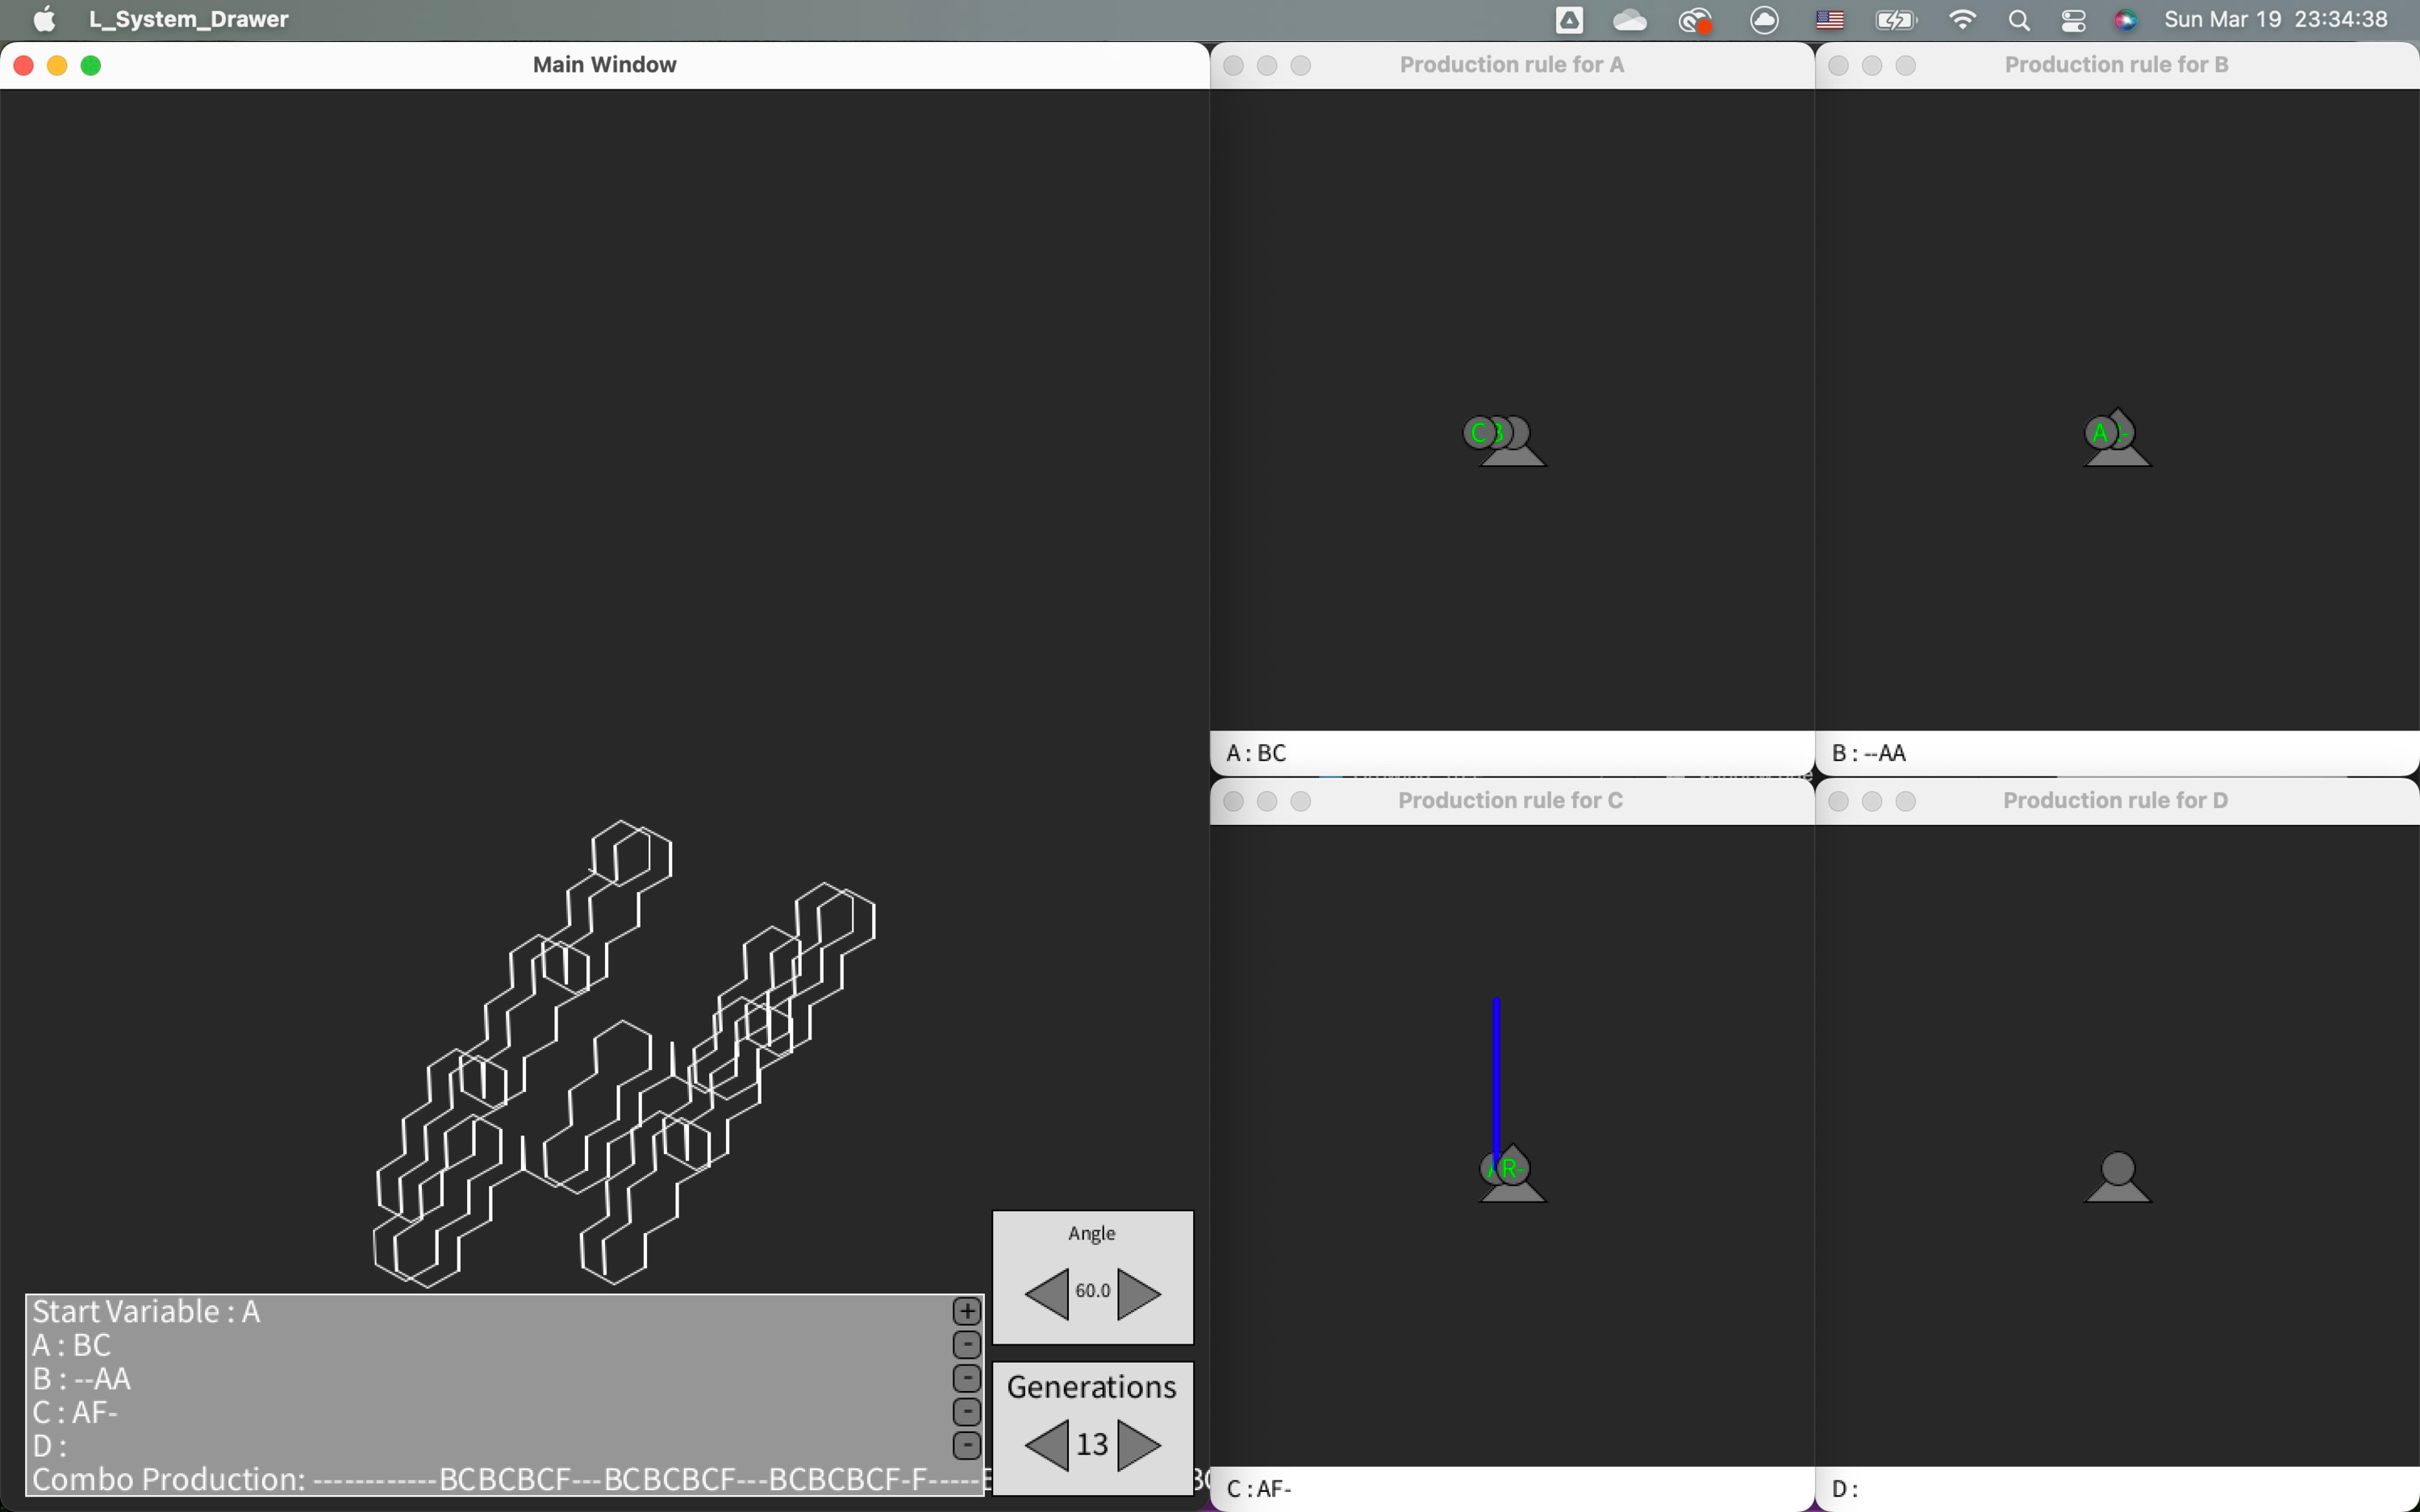
\includegraphics[scale=0.3]{Images/EarlyExplorer}
	\caption{An early version of the Explorer}
	\label {EarlyExplorer}
	\end{figure}

	The development of the L-System Explorer started with a series of drawings describing the different features I was aiming to include. I wanted everything to be able to be accessed without touching the keyboard. There have been a few moments since I started development on this project where things could have been easier if typing was allowed, but so far I only expect one of those uses to actually need the keyboard. (I was imagining that if someone wanted to input an L-System that they already had on hand, it would make sense for them to be able to type it in. [put this in a footnote]) Once I had a set of features in mind, I began to write the program.
	
	I built the windows first. There is a main window that displays the current visualization of the L-System and one smaller window per active production. These sub-windows are created and removed to keep in line with the number of productions. In the basic processing version of the Explorer, the windows for the productions are able to be moved independently from the main display window. From there, I began to build up the framework of the Explorer itself. Keeping the goal of approachability in mind helped prevent me from making the program too dependent on any specific programming experience. Although this thesis adds depth and context to the program, I hoped to make the Explorer self-explanatory enough to operate without having to read this document. The structure of the Explorer changed throughout its development and continues to change, but I'll describe the form that it has taken at the time I'm writing this.
	
	%\textcolor{blue}{[A screenshot of the most updated version I can include]}
		
	\begin{figure}[h]
	\centering
	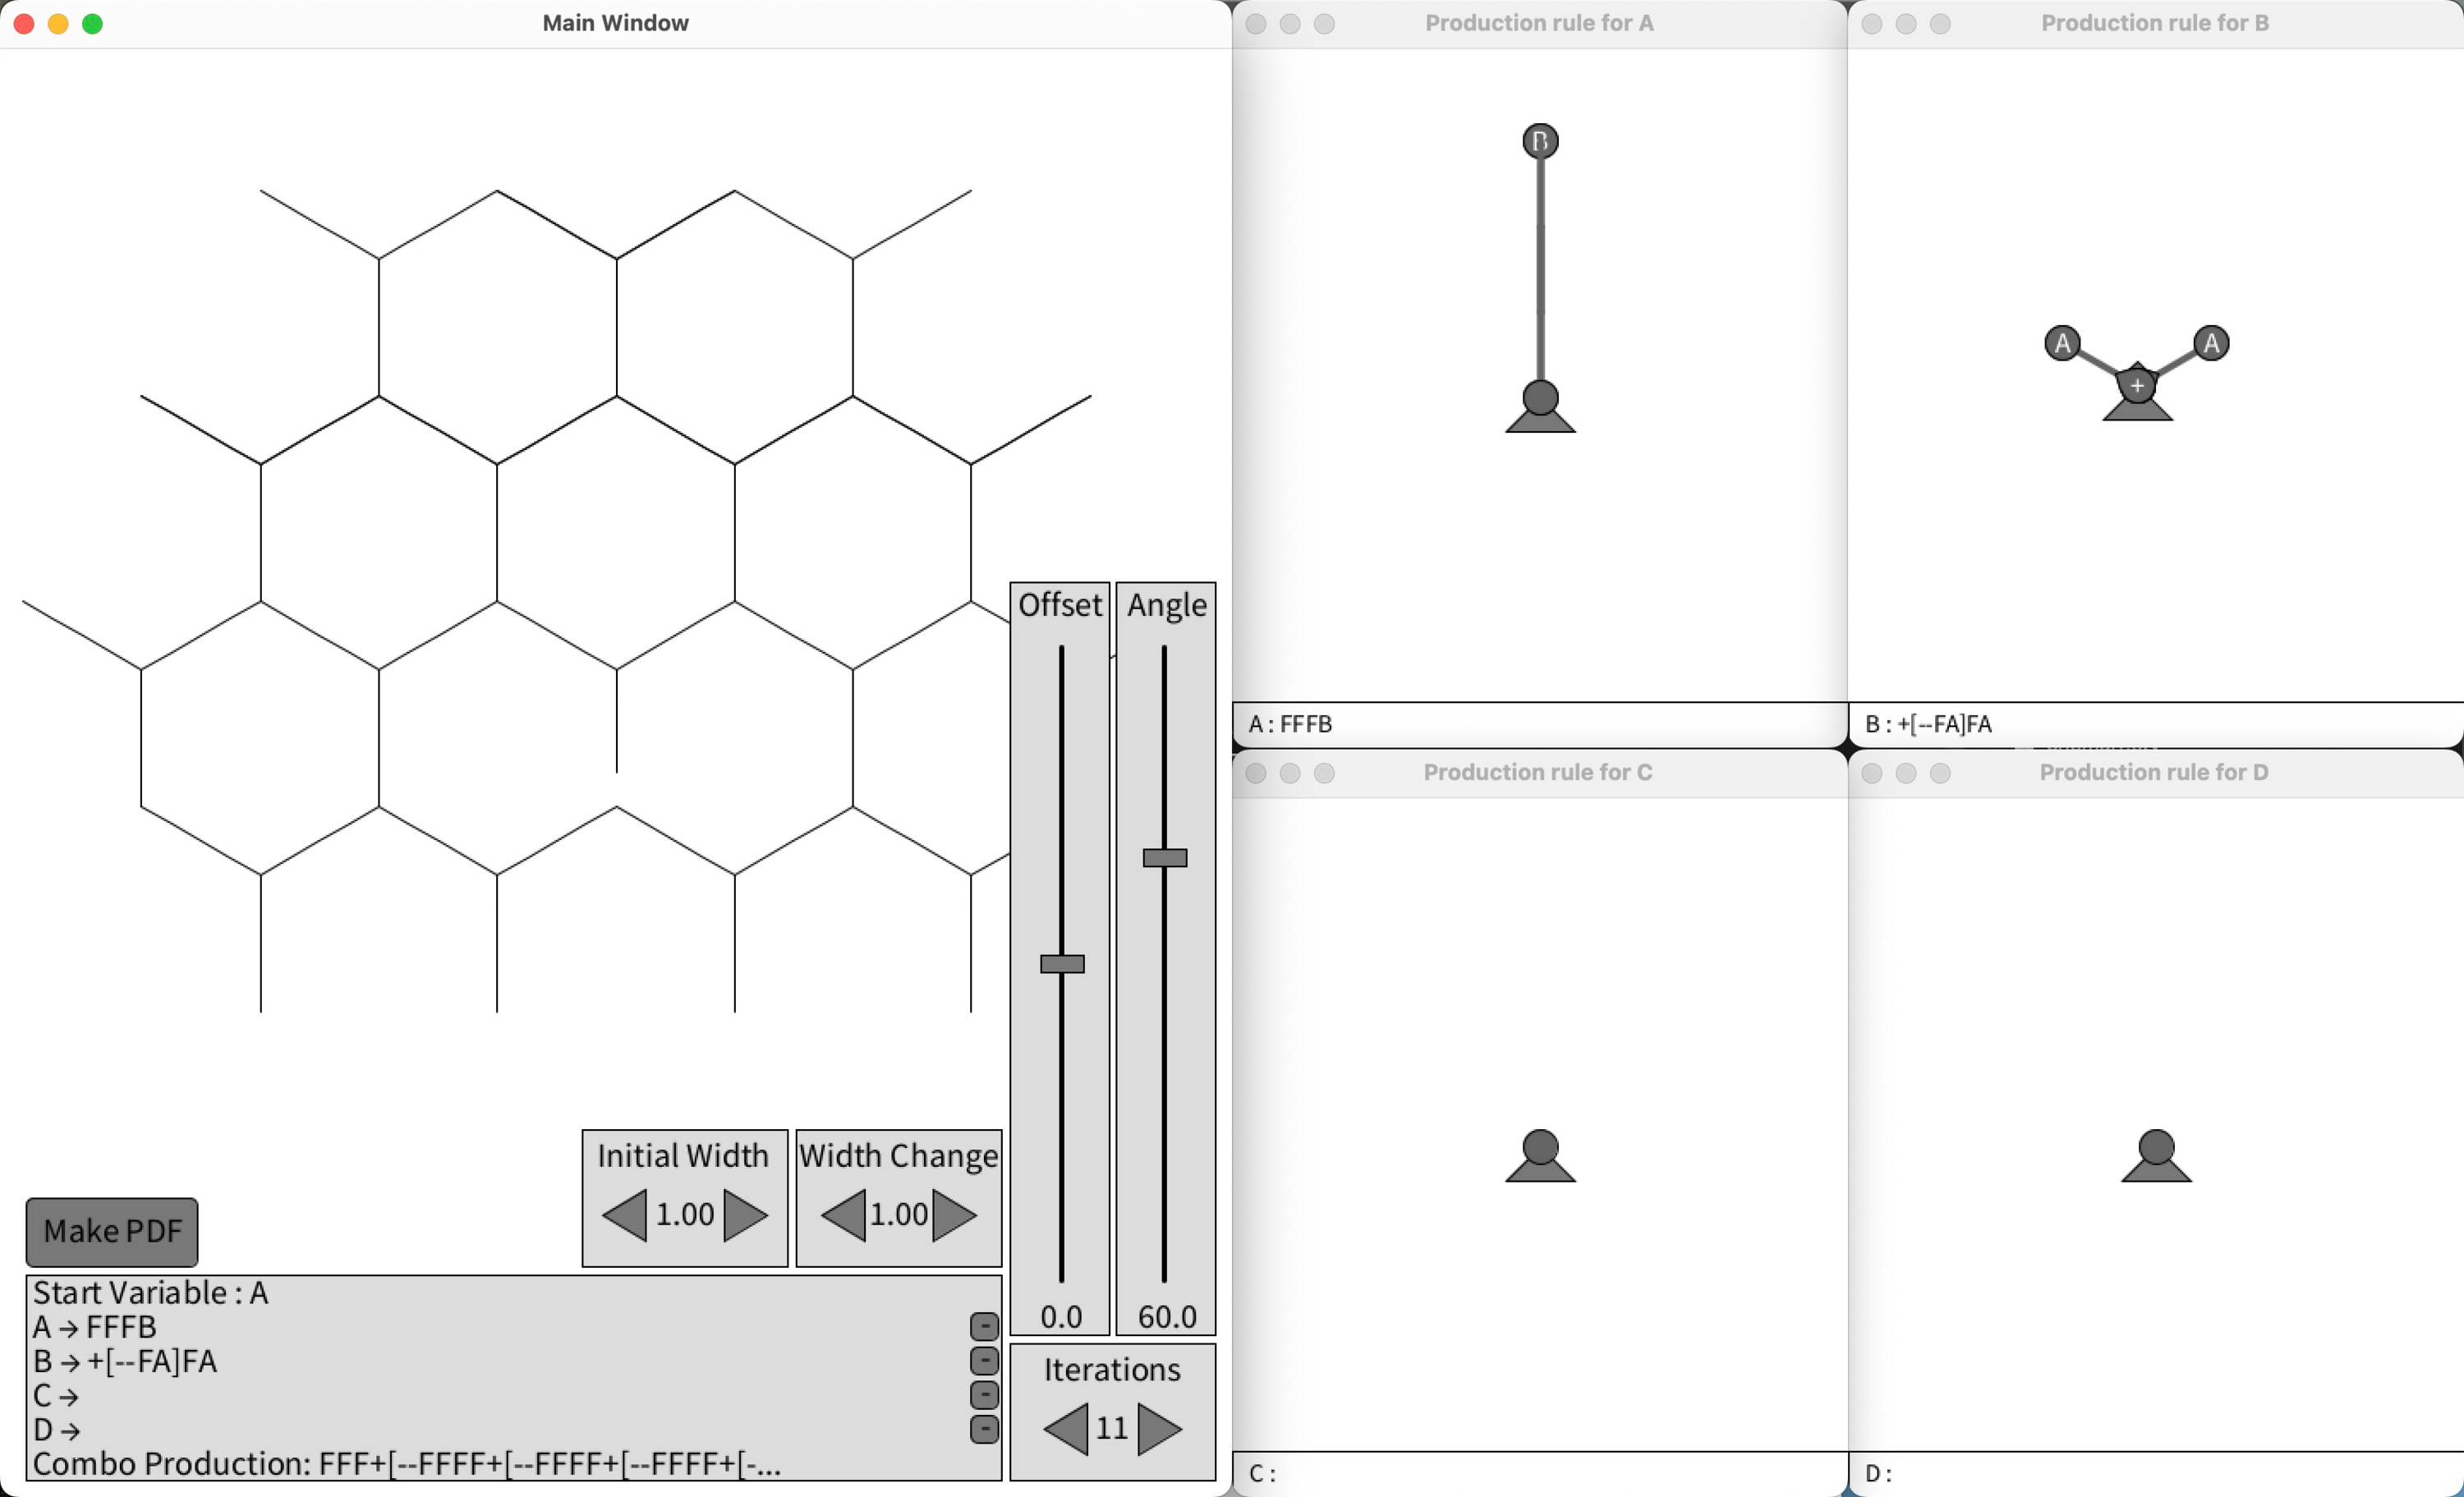
\includegraphics[scale=0.3]{Images/CurrentExplorer}
	\caption{The current version of the Explorer}
	\label {CurrentExplorer}
	\end{figure}
	
\section{How it works}

	I talk about the details of the L-System Explorer in this section. I would encourage you to read on if you're interested in taking a look under the hood about how I brought it to life. However, there won't be any new concepts regarding L-Systems introduced here. To move past this and get a summary of how to use the program, go ahead to Section \ref{Using-the-L-Systems-Explorer}.
	
	%\textcolor{blue}{[Empty main window and empty sub-window]}
	\begin{figure}[h!]
	\centering
	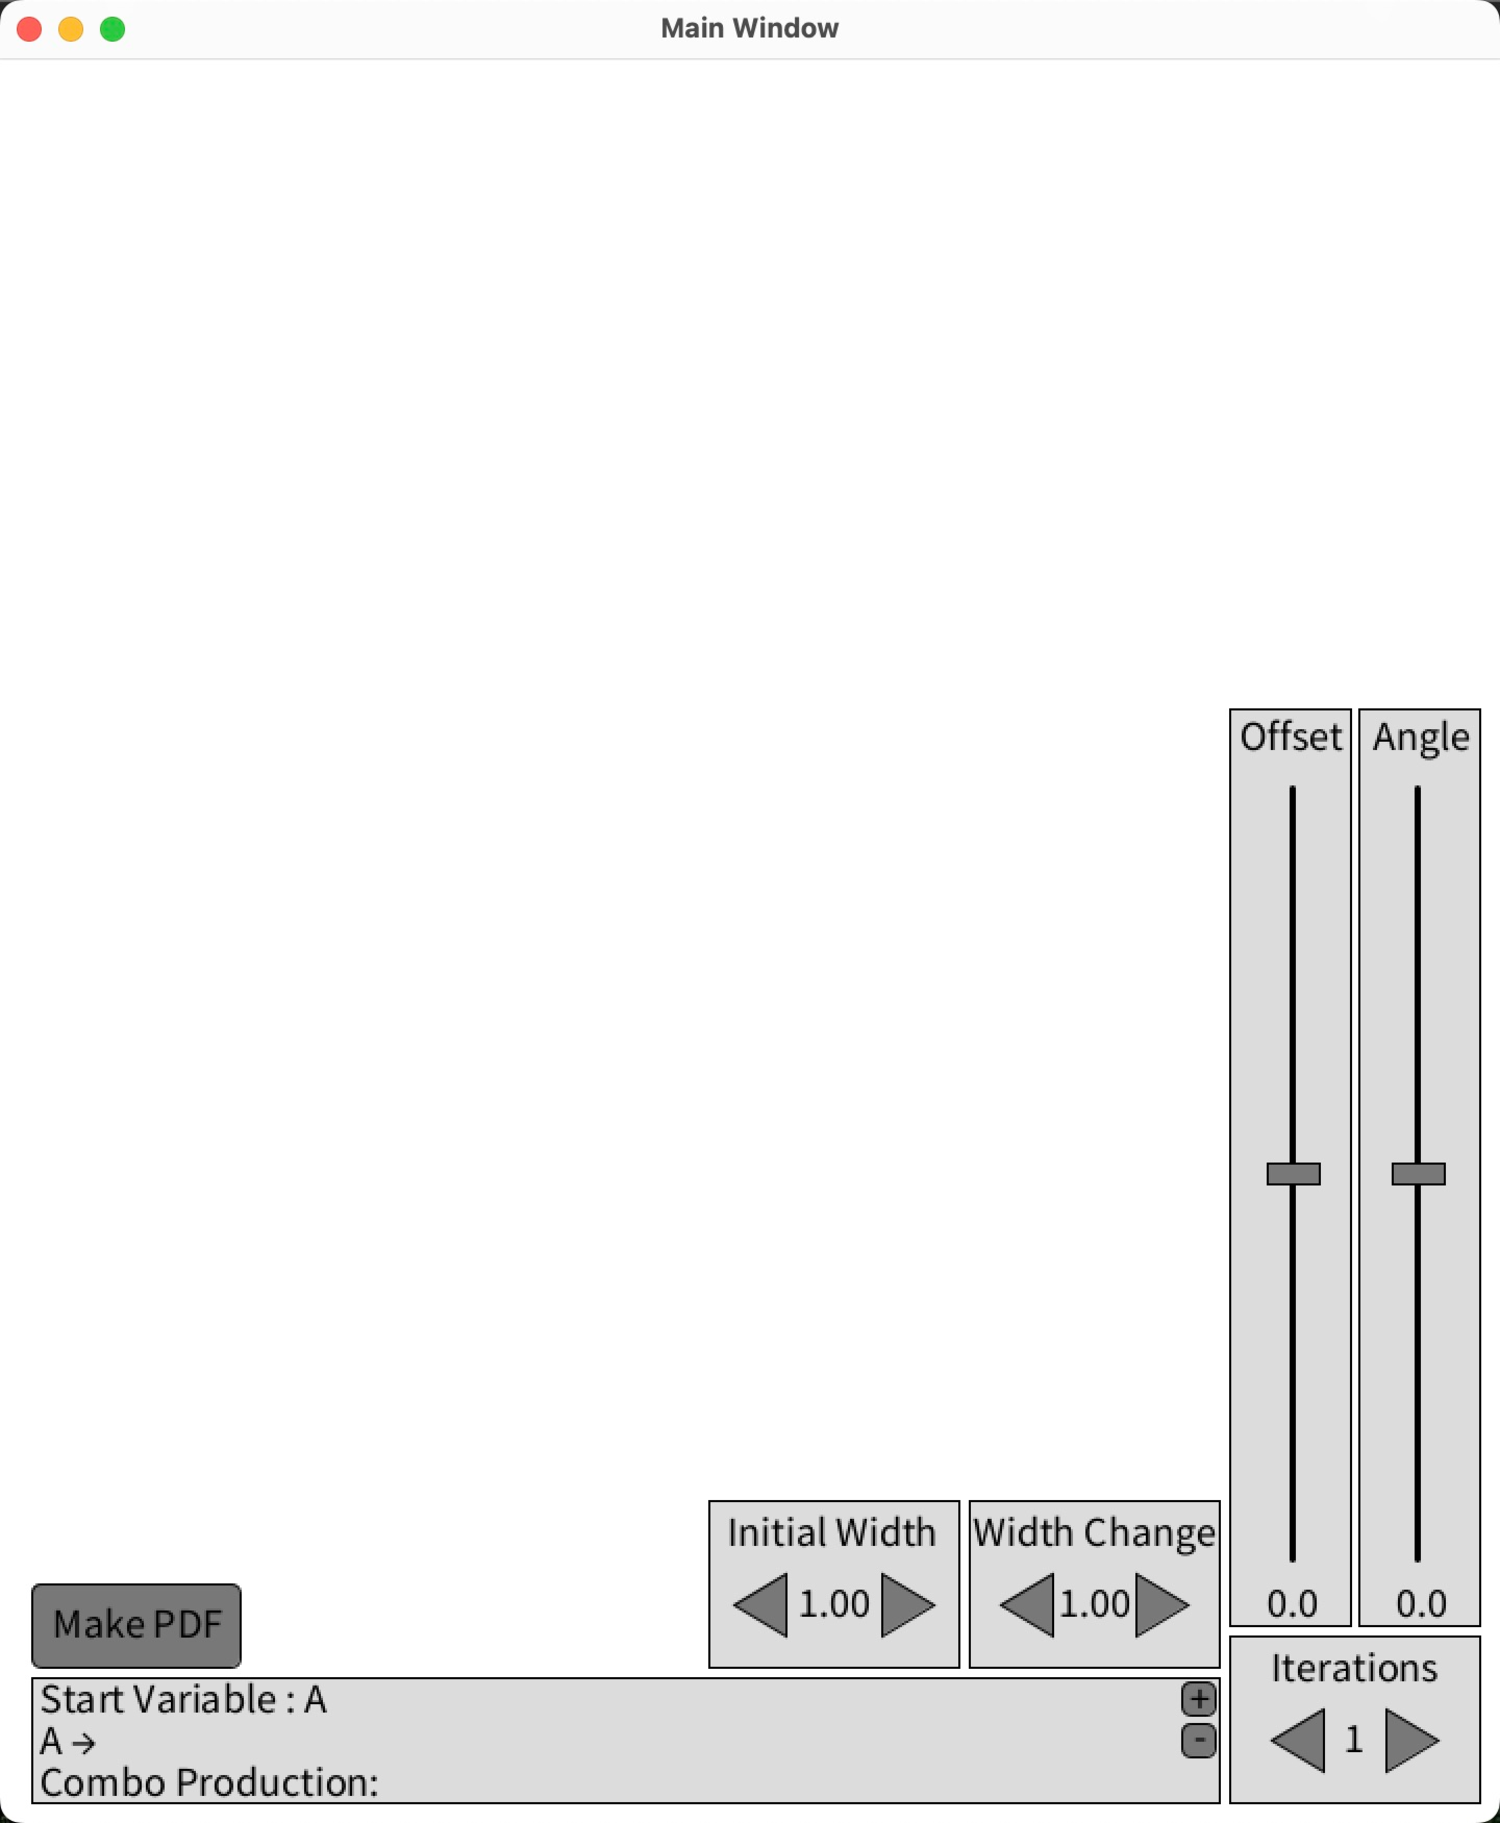
\includegraphics[scale=0.5]{Images/HowItWorks1}
	\caption{The Main Window}
	\label {MainWindow}
	\end{figure}

	
	The main window is initialized upon startup. Some number of sub-windows, one for each production that the program starts with. More productions can be added, and more windows are created for productions when needed. Windows are similarly removed when not needed. Each sub-window contains a reference to a `starting' triangle that I fittingly named the \code{StartTriangle}. This is an instance of a class that can be moved up to the boundaries of its window. The start triangle has a reference to the \code{startNode}, which is the root of a linked list structure of nodes. I've made a class to describe the nodes as well. When the \code{StartTriangle} is moved, the \code{startNode} is moved similarly, and then recursive calls down the node tree move all the nodes to the correct positions. Each \code{StartTriangle} and its closely-tied \code{startNode} provide the foundation on top of which each of the production rule displays are constructed.
	
		
	\begin{figure}[h!]
	\centering
	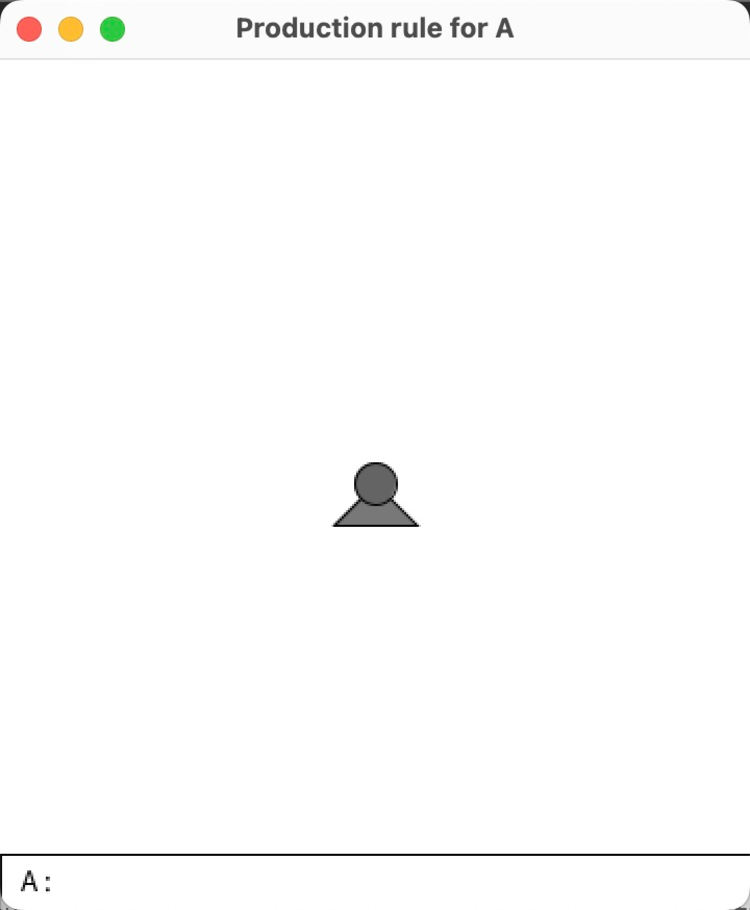
\includegraphics[scale=0.5]{Images/HowItWorks2}
	\caption{A sub-window}
	\label {Sub-Window}
	\end{figure}
	
	%\textcolor{blue}{[Start Triangle and Start Node]}
	\begin{figure}[h]
	\centering
	
\includegraphics[scale=1]{Images/HowItWorks3}
	\caption{The \code{StartTriangle} and the \code{StartNode}}
	\label {HowItWorks3}
	\end{figure}
	
	There are five subtypes among the node class, each node belongs to only one of these subtypes. These aren't subclasses, the different nodes have some different functionality, but they're only differentiated with a string. The start node is the only element of the \code{start} subtype; I use this as a signpost to stop calls from nodes to their parents from going too far. There are \code{production} and \code{rotation} nodes, the main difference being that rotation nodes have a point that shows which direction they're oriented. The fourth subtype is \code{forward} nodes. These are displayed as lines, unlike the other types of nodes, which are displayed as circles. The final subtype is \code{option} nodes. These are a special type of node with some unique characteristics. They have a pointer to an \code{optionParent} node, which may be a member of any subtype of node, including another option node. They will only appear if their \code{optionParent} node is being hovered over by the mouse or their \code{optionParent} has recently been hovered over by the mouse and the mouse has not left its vicinity or the vicinity of any of its \code{option} nodes.
	
	%\textcolor{blue}{[Images that show how the mouse interacts with the nodes]}
	\begin{figure}[h]
	\centering
	\begin{subfigure}{0.5\textwidth}
		\centering
		
\includegraphics[height = 2.5in]{Images/HowItWorks4A}
		\caption{Mouse near a node}
		\label {HowItWorks4A}
	\end{subfigure}%
	\begin{subfigure}{0.5\textwidth}
		\centering
		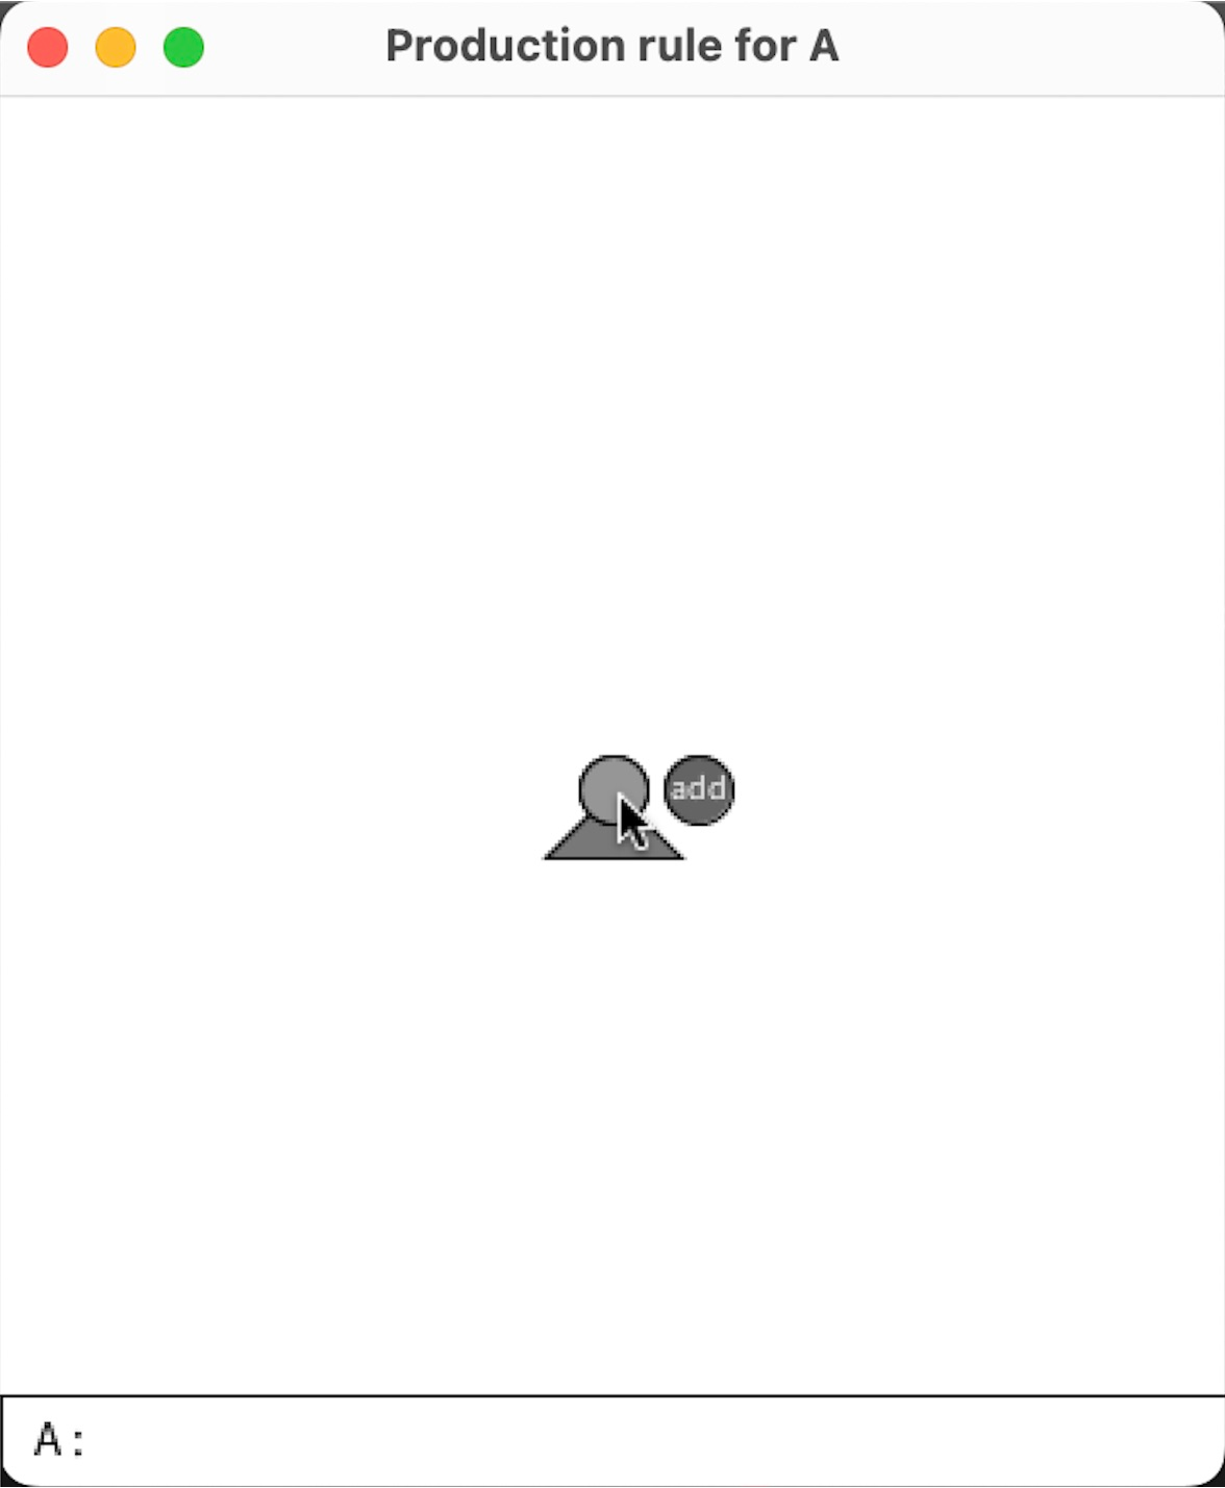
\includegraphics[height = 2.5in]{Images/HowItWorks4B}
		\caption{Mouse over a node}
		\label {HowItWorks4B}
	\end{subfigure}
	\begin{subfigure}{0.5\textwidth}
		\centering
		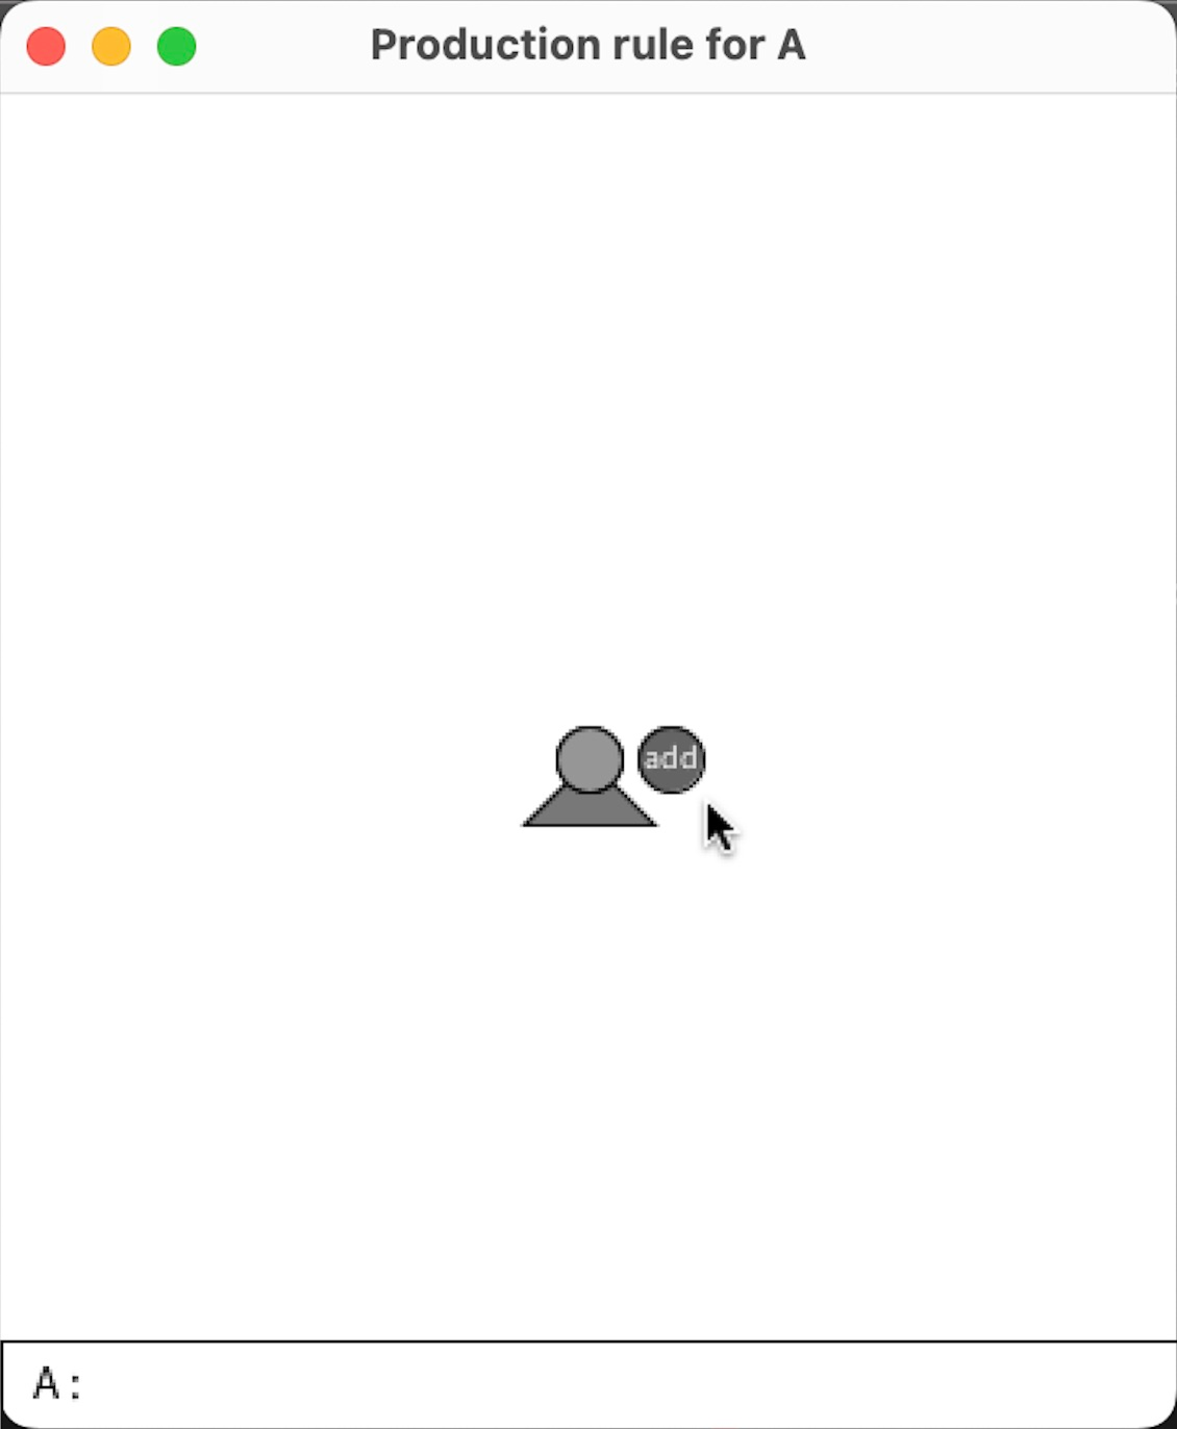
\includegraphics[height = 2.5in]{Images/HowItWorks4C}
		\caption{Mouse nearby after being over a node}
		\label {HowItWorks4C}
	\end{subfigure}
	\caption{Mouse interactions with nodes}
	\label{MouseInteraction}
	\end{figure}


	Each node of any subtype can only interact with its neighboring nodes and the \code{option} nodes that refer to it as an \code{optionParent}. This intentionally limited functionality is created by giving each node a pointer to one other node in the direction of the \code{start} node. This is the node's \code{before} node. It also has an array of \code{after} nodes, which consists of all the nodes that consider this node to be their \code{before} node. The remaining reference in a node is the array of \code{option} nodes that consider this node to be their \code{optionParent}.
	
	%\textcolor{blue}{[An image of the options, with the mouse hovering over an \code{optionParent} node]}
	
	\begin{figure}[h]
	\centering
	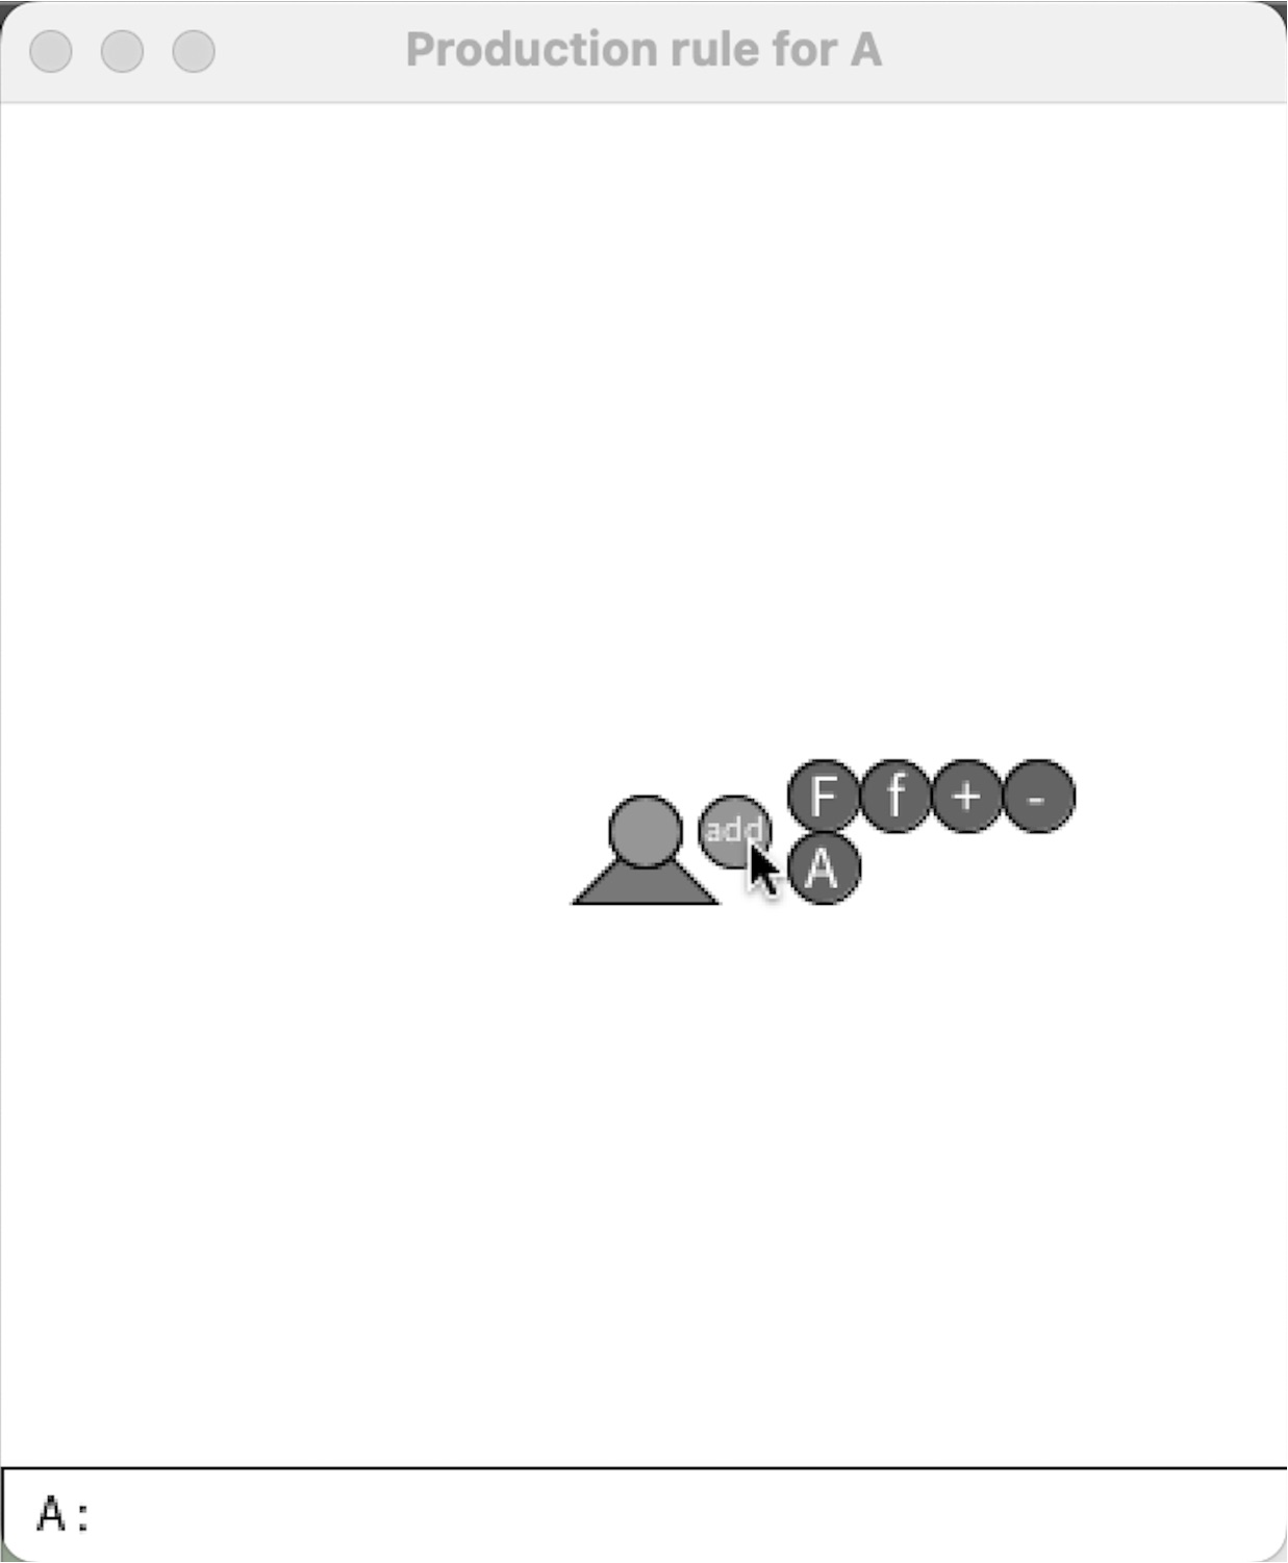
\includegraphics[height = 3in]{Images/HowItWorks4D}
	\caption{Multiple nodes}
	\label {HowItWorks4D}
	\end{figure}
	
	\textcolor{blue}{[A diagram of the relationships between these nodes]}
	
	
	
	Beyond the references, each node contains information that defines its state. One part of a code's state is the value \code{over}, which is a boolean for whether the mouse is over the node. Another main event is \code{press} which is a boolean for whether the mouse is clicking the node. The most central variable is called \code{activated}. \code{activated} is a boolean with a complicated condition. It corresponds to whether the mouse is currently over the node or was recently over the node and has not moved too far away. If \code{activated} is true, then some user interface logic ensures that no other node is activated or can become activated while this node is activated. This happens through a recursive method called in a node's \code{before} node and its \code{after} nodes. \code{option} nodes are the exception to this. They will only ever be \code{activated} when their \code{optionParent} is already \code{activated}. Each node also tracks its position and orientation, information that is referenced by this node's \code{after} nodes to ensure that every node is in the correct state.\\
	
	\textcolor{blue}{[A diagram of the recursive-ness of the code that ensures that all the right nodes are activated]}\\
	
	There are specific ways for users to engage with this process. The user is able to click on the \code{option} nodes of an \code{activated} node, and if the node has an associated action and some conditions are fulfilled, the action happens. Usually, this action is the creation of a new node whose \code{before} node is set to be the current node (the node whose \code{option} node was just clicked). The other case is that the \code{option} node that was clicked will trigger the deletion of that \code{option} node's \code{optionParent} node. For both of these possibilities, the current node's \code{after} array and the display are both updated.\\
	
	\textcolor{blue}{[Two images showing how the deletion of a node affects the arrays and display (maybe actually four images? Two that show what is on the screen and two that show the changing relationship of the nodes behind the scenes?)]}\\
	
	 Each sub-window has a function to turn its tree of nodes into a string that uniquely describes it. This is done through a process of depth-first search, where each branch of the tree is explored down to its end, adding elements to the string as it does. The tree is explored through the \code{before} and \code{after} linkages. Any time the tree branches, the function adds an \code{[}, and any time the tree finishes reading a branch, the function adds a \code{]}. These brackets allows complex branching structures to be accurately described in only one string. Most nodes have an associated character that is added to the string whenever the node is seen on the tree. \code{rotation} nodes have either a \code{+} or a \code{-}. \code{forward} nodes have either an \code{F} or an \code{f}. \code{production} nodes have the character of their associated production. (These might be \code{A}, \code{B}, etc.) The \code{start} node and \code{option} nodes are not read by the function and so do not have associated characters. At the end of this process, the sub-window has a string that is the production rule for the production of that sub-window.\\
	 
	 \textcolor{blue}{[Images showing the creation of a string based on some L-System]}\\
	
	Similar to how each node's \code{after} nodes will have a way to access their \code{before} node, each sub-window is able to access some information from the main window. The main window is also able to change some information in the sub-windows. However, there is no way for the main window to directly affect the start triangle or nodes within any of the sub-windows. It must have each sub-window do that. Some information must still be transferred between layers, information such as the production rules. The main window is able to reference the production rules from each sub-window. It applies the L-System recursive replacement process described in section \ref{Understanding-through-Images} some number of times equal to the value of \code{Iterations}. This value can be changed by the user. The output of this process is the L-string, which is used to draw the L-System.\\
	
	\textcolor{blue}{[A labelled drawing of the different strings and how they are related between the different windows]}\\
	
	In the process of drawing the L-System, the Explorer reads the L-string character-by-character and performs actions depending on that character. It acts very much like Turtle Graphics described in section \ref{Turtle-Graphics}. It also has another data structure called a ``stack". The Explorer is only allowed to interact with the top item on the stack, and it can choose to read it or to remove it. It can also add a new item to the top of the stack. (It cannot add a new item in the middle.) In this case, the kind of item that we're putting on the top of the stack is a snapshot of the current state.\\
	
	\textcolor{blue}{[An illustration of the Explorer's stack and how the system engages with it]}\\
	
	When the Explorer processes a \code{[}, it puts the current state onto the stack. Whenever it processes a \code{]}, it sets the current state to the state that is on top of the stack, then it removes the state on the top of the stack. If it processes an \code{F}, it goes a given distance in the direction it's facing and draws a line between its starting and ending point. When it processes an \code{f}, it goes that distance in that direction, but doesn't draw a line. A \code{+} adds the given angle value to its stored orientation. \code{–} does the same, but subtracts the angle from the orientation instead. The angle can be changed by the user to quickly see different possible views of the L-System. Reading a production like \code{A} or \code{B} doesn't change its state, nor does it draw anything. It won't change its state if the character that it reads is not among these ones.
	
	While this could certainly be less complicated, I feel proud to have been able to make a system that feels to me to be relatively sleek and clear in its purpose. It does succeed in hiding much of its complexity under the hood to give users as simple an experience as possible. It was shocking and yet strangely affirming to experience the intricacy of building a user interface. This was an invigorating exercise in articulating exactly what I want from the program. It was so wonderful being able to see where there were mistakes in my understanding, as the program would very explicitly tell me.

\section{Using the L-Systems Explorer}
\label{Using-the-L-Systems-Explorer}

	This project has what I feel is necessary to get a basic understanding of L-Systems. There were many judgement calls in the design of the work, though I hope that this program has achieved what I set out to do.\\
	
	\textcolor{blue}{[An image of the github page with the files and the processing website with all the relevant areas emphasized]}\\
	
	To access this program, you need to download both the program and the framework to support it. The program can be downloaded at \textit{github.com/RJacobH/Thesis}. You will need the four files, \code{L\_Systems\_Explorer.pde}, \code{Helpful\_Functions.pde}, \code{Node.pde}, and \code{Window.pde}. Download these and put them in the same folder. Next, go to \textit{processing.org} and download Processing. At the time that this was written, this program works in Processing version 4.2. From here, you can open any of the four files you just downloaded and you should something that looks like the image below. Click the play button in the top left corner and get started exploring!\\
	
	\textcolor{blue}{[An image of the screen when the program is opened]}
	
	%To access this program, go to ``rjacobh.github.io/website" and click on the tab on the top of the page that says ``Processing".\\ % This is assuming I successfully manage to put the program on my website. :8| We'll see
\subsection{How to Explore}
	
	
	\textcolor{blue}{[Give images for each of the following steps]}\\
	
	The first time you use the L-Systems Explorer, hover over any of the circles in one of the smaller windows. When you do this, you'll see several more circles appear, each with a different symbol inside of them. These are buttons. Clicking on the button that says \code{F} will cause a line to appear on the small screen as well as the larger screen. Hover over the new line in the small window and click the \code{+} button. This creates a new shape in the small window. Hover over this new shape and click the \code{F} button that appears. This will make another line appear in both the small window and the big window. You can see the production rule of the small window running along its lower edge. Also notice how the title of the window is ``Production rule for A". Creating these elements has changed the production rule for \code{A}.\\
	
	\textcolor{blue}{[Give images for each of the following steps]}\\
	
	Look for a slider that says ``Angle" on the right side of the page. Moving this slider, you'll see your lines move. Try going back over to the small window and hovering over the second line you drew. It doesn't need to be vertical. Click the button that pops up that says \code{A}. Now find the box that says ``Iterations" in the bottom right corner of the large window. Click the triangle that points to the right. You'll see the number in the box go from 1 to 2, and the size of your line in the big box get much longer. Try clicking the rightward-facing triangle a few more times. Also try moving the angle slider. Look at what's happening!\\
	
	\textcolor{blue}{[Give images for each of the following steps]}\\
	
	From here, you can go back to the small window and hover over the first line you drew. Click the \code{–} button that appears. Now hover over the new \code{–} node and click its \code{F} button. Hover over this new line and click its \code{A} button. If your Iterations box says 1, increase it. Move the angle slider and see what's happening. Move the slider that says ``offset" and see how that changes things. Try changing the production and seeing what interesting shapes you can produce.\\
	
	\textcolor{blue}{[Give images for each of the following steps]}\\
	
	The last essential thing to learn about this program is how to add more productions and production rules. Look for a box that says ``Productions". Click on the small \code{+} box. A new small window should appear. The original small window continues to correspond to the production rule for \code{A} and this new window will correspond with the production rule for the new production \code{B}. You can reference \code{B} within the \code{A} production rule window and vice-versa. One final point, you can stack rotation nodes by hovering over a rotation node (\code{+} or \code{–}) and clicking the button for the same type of rotation node. Choosing the other direction of rotation node will cancel its effect but choosing the same type will double the effect. This can be repeated any number of times. Some of the most interesting L-Systems I've found have used this effect.\\
	
	\textcolor{blue}{[Provide as many interesting initial inputs as I can justify, perhaps 6? Show some techniques used to great effect.]}

\chapter{Contribution}
	A primary goal of this work is to make L-Systems, and by extension Generative Art and Computer Science broadly, more approachable. This is not the only goal. I want folks who haven't used computers as an artistic tool before to create things in this medium. I even want my peers, who have been immersed in the depths of CS for years, to be able to approach the discipline with a fresh awe and changed understanding. I want everyone to be amazed and inspired by the possibilities and to feel capable of creating their own new work.  I feel that these are all very attainable without having to engage with the complexity of modern design software.
	%like Blender, Photoshop, Fusion 360, or others, though those absolutely have their place.\\
	
	Keeping in mind that L-Systems were proposed back in 1968, I was worried that with 55 years to develop these ideas I wouldn't be able to tread on any new ground. This is true in many respects, and I re-emphasize that a main goal of this work is to raise awareness of L-Systems and to bring together some sources that discuss these ideas at the level of an undergraduate thesis. However, this work goes a little beyond that. There are few implementations that make L-Systems easy to play with. Even those who brought L-Systems to Blender still only make them available to those who know Blender.\footnote{\cite{Leopold2017}}
	
	This Blender work I mention is incredible, and I found it a great source of inspiration, but our projects have fundamentally different goals. As far as I'm aware, no other program has made L-Systems this easy to play with, despite the central part of their appeal being simplicity. As far as I can tell, there has been no easy way to gain an intuition with these systems that isn't locked behind years of engagement with computer science.\\
	
	\textcolor{blue}{[Some sliders, the parts of the program that are especially simple]}\\
	
	My central contribution has been the development of the interactive L-System Explorer. I hope that it's clear that this project will be able to engage with people, no matter their experience with computer science. I hope that this ability to craft L-Systems will help those who are interested to overcome any wariness about engaging with digital machines as an artistic medium. Despite computer science being about much more than pretty pictures, I feel that a warm welcome will help those who were once strangers come into this place as their home. These pictures and this thesis are my attempt at creating a warm welcome.

\section{Related Work}
	I wrote three main programs for the generation and display of L-Systems. These are a native Python program, an implementation of that program embedded in Blender, and the final L-System Explorer described in detail in this thesis. These projects were interspersed with a research process that involved investigating other implementations of L-Systems and related topics. I'll discuss a few of those related topics here before expanding the discussion to include other visual structures that I feel are worth exploration.\\
	
	\textcolor{blue}{[Three images that show the three programs in action]}\\

	The 1990 book \textit{The Algorithmic Beauty of Plants}\footnote{\cite{ABOP1990}} grounded my study from the beginning. This opened my eyes to the beauty of L-Systems. I recommend the free version that is available online, as the book is now sadly out of print. The book is a font of compelling diagrams and images of fairly convincing computer-generated plants. It would be worth a look purely to see the pictures of plant created with L-Systems.\\
	
	\textcolor{blue}{[Some images from ABOP]}\\
	
	Another useful resource for me has been the YouTube channel \textit{The Coding Train},\footnote{\cite{codingTrain}} and I'm grateful for the wide variety and expansive content of their videos. They were my introduction to some of the ideas that I talk about more in the following Generative Art section, and they're responsible for much of my foundational learning about Processing. If you have an interest in taking the next step in your computer science journey, I would highly recommend these videos, especially the tutorials on getting started in Processing. I would be hard-pressed to find a better resource than this channel. I've followed along many of the tutorials and discovered some fantastically interesting concepts that I hadn't come across in school, such as Perlin and Simplex noise, strange attractors, and space-filling curves.\\
	
	\textcolor{blue}{[Some images from the Coding Train]}\\
	
	Nikole Leopold wrote a Bachelor's thesis about an implementation of L-System graphics in Blender in 2017 at the Technical University in Vienna.\footnote{\cite{Leopold2017}} This work informed some of the later discussions that I've had as part of this thesis. Leopold gives a comprehensive overview of the advantages of using a 3d modeling software like Blender to display L-Systems. They also introduce an add-on which enables the user to immediately see the results of their changes, a strategy I admire and have worked to make an essential component of my own project. One of the pieces of that research that I found especially interesting was the inclusion of methods by which the L-System can interact with its environment. The structure grows, finds an obstacle, and appears to go around it. (The program actually just cuts off the branches that intersect the object, but the effect is still compelling.) The discussion of Differential L-Systems was also fascinating. These are L-Systems which can be animated continuously, by which I mean \textit{between} production steps. [Include some footnote about how cool this is - it's animation to a crazy degree!] I'm grateful for the resources that Leopold included as well, as they pointed me in the direction of additional compelling sources.\\
	
	\textcolor{blue}{[Some images from Leopold's paper]}\\
	
	Przemyslaw Prusinkiewicz, who worked with Aristid Lindenmayer on \textit{The Algorithmic Beauty of Plants}, produced a handbook in 2001, titled \textit{L-Systems: from the Theory to Visual Models of Plants}\footnote{\cite{LSystems2001}} that I view as something of a sequel to the work presented in \textit{ABOP}. It goes into depth on some of the ideas presented in \textit{ABOP} but with new pictures that bring wonder in all the right ways. It discusses different forms of L-Systems, a few of which I discuss in the next chapter. It also explores hypothetical models that I'd never considered, such as simulating an attack on a plant by an insect, and displaying how the system reacts.\\
	
	\textcolor{blue}{[Some images from this text]}\\
	
	Finally, the paper ``A Theory of Animation: Cells, L-Systems, and Film" goes well beyond the scope of this thesis in its discussion.\footnote{\cite{theory2004}} It provides some insight that's more helpful for the larger questions that have been raised during this process, and less about the structure of L-Systems. It suggests a view of L-Systems and similar structures as ``animations of a \textit{theory} of cellular life." (32) This is especially interesting to me in the context of the discussion of the alive-ness of machines, and the degree to which a machine that simulates life can be said to actually \textit{be} life. I ask these questions more clearly a bit further on in section \ref{Questions}. This paper is also interesting to me for the degree to which it ties popular culture to these simulators. It is cross-discipline in the most appealing way.\\
	
	\textcolor{blue}{[Some related image? (perhaps not, this'd be filler)]}\\
	
	Another class of life simulator that's often grouped with L-Systems is the field of Cellular Automata. These structures surpass L-Systems in terms of simplicity, often operating in a simple grid or even just a line of points. Popular examples are John Conway's \textit{Game of Life}\footnote{\cite{GameOfLife1970}} and Stephen Wolfram's one-dimensional Automata.\footnote{\cite{wolfram2002}} These have been used alongside L-Systems to generate life-like effects for film and other media for a long time.\footnote{\cite{theory2004}} Their simplicity also makes them a great tool for creating emergent systems and acting as simple models for complex behavior. They can also demonstrate a remarkable capability for beauty, which I will discuss in more depth now.

\section{Generative Art}
\label{GenerativeArt}

	People have been fascinated by the cooperative creations of human and machines for as long as such things have been able to be made. Many of these creations are seen as \textit{beautiful}. These structures don't necessarily have to conform to traditional standards of beauty, but they do look usually look like what we know as \textit{art}. These works just happen to be created in part by machines. One section of the creations made by machine but under some human assistance fall under the label \textit{Generative Art}. For the purposes of this thesis, I will define Generative Art as art that comes from a machine with the guidance of a human.
	
	With only a little searching, I've found several online communities that create beautiful collections of this work.\footnote{\cite{reddit2023}} I've also been fortunate to be near many people that are also interested in many of these same ideas and have supported me in this work more actively. I credit Trever Koch for helping me bring many of my early ideas to life. The point here is that there are resources available if you are at all interested in learning more about this. I have collected specific resources and put them in Appendix B for your perusal.\\
	
	\textcolor{blue}{[Some weird \& different Generative Art things]}\\
	
	There is a huge variety of work that could be considered Generative Art. The art made by systems like DALL-E, MidJourney, and other AI programs might fall under some definitions of Generative Art, but it feels distanced enough from the material that I'm interested in covering here that I'll isolate them to a discussion in section \ref{AI-Art}.\\
	
	\textcolor{blue}{[One or two AI art things (maybe don't include this? Ethical concerns?)]}
	
\subsection{My Explorations} % Should this be its own section?
	
	I explored a variety of systems for creating artwork with machine means during the first stages of my research process. I'll introduce some of those structures here and demonstrate how they tie into the theme of simulating life. Each of these projects are deserving of greater research in their own right, and so I won't attempt to make my explanations comprehensive. This section I hope you enjoy these objects as both the artworks and the mathematical structures that they are.\\

	Here are some of the chronologically earliest projects that I explored. These were made in a program called OpenSCAD (pronounced ``open S cad") and were a first attempt to create artworks through software.\footnote{\cite{openSCAD}}\\
	
	\textcolor{blue}{[OpenSCAD projects]}\\
	
	This is a ``mesh" that I was messing around with during these early stages as well. I was curious if I would be able to modify it so that I might be able to fold paper into a physical model. This particular version never came about.\\
	
	\textcolor{blue}{[Head Mesh]}\\
	
	However, I did manage to create a few physical models of geometric solids.\\
	
	\textcolor{blue}{[Paper icosohedra]}\\
	
	These fall into the category of ``papercraft", a medium that I feel especially connected with. The L-Systems that I've been showing off take a line and brings it into the 2nd dimension. These papercraft objects bring 2d objects into the third dimension. These paper models are descendants of a series of creations that I've been making years before embarking on this thesis project. Here are some examples of those.\\
	
	\textcolor{blue}{[Modular Origami] (If you're interested, these specific types of objects are part of a discipline called ``Modular Origami".)}\\
	
	I've already mentioned my early explorations into the native python implementation of turtle. Here are some of the systems constructed during that time.\\
	
	\textcolor{blue}{[Early turtle SVGs]}\\
	
	At this point, I began to explore the possibility of bringing L-Systems into the third dimension. I used Blender and an implementation of Turtle Graphics that I constructed to build complex 3d shapes. My favorite of these is probably the 3d Hilbert Curve, in part because it made me consider how the turtle works. In a sense, the turtle doesn't move through its world, instead the world moves around it.\footnote{\cite{derose1989}} This is a part of this process that would be very fun to explore further, especially with the knowledge from a paper that I came across later in the process. Here is the Hilbert Curve and a few other 3d constructions from L-Systems.\\
	
	\textcolor{blue}{[3d Hilbert Curve and others]}\\
	
	It was at this point in the thesis that I encountered Processing. Here are images of some of the projects that I made as part of this particular exploration. Note that most of these are snapshots of a program in motion, and a lot of detail will be lost when we remove the time dimension. I would like to put some of these on my website at some point to let those who are interested to experiment.\\
	
	\textcolor{blue}{[Stills from Processing animations, definitely the Simplex Cloud]}\\
	
	These projects were instrumental to the development of the thesis as you see it now. Without considering them, an understanding of my thesis is incomplete.

\section{Quandaries, Puzzlements, and Musings}
\label{Questions}

	While working on this thesis and the various projects that came with it, I began to begin to see things through a peculiar lens. I was researching this type of structure that had been used for half a century to describe living things with an almost startling degree of accuracy, considering the simplicity of their construction. I started to question the line between living things and the code we write to imitate those living things. Is there actually a difference? I'm not so sure. I'll share where my thinking has been going these last few months over the course of this section.
	
	This is the sort of question that people have been asking for hundreds, if not thousands of years. Machine-makers have attempted to imitate life by different means for a similarly long period.\footnote{\cite{riskin2016}} Science Fiction authors and pioneers like Alan Turing have suggested ways in which we might learn if there is a difference between life and machines.\footnote{\cite{turing1936}} Some of those questions have borne fruit or guided our development, others have marked moments when we moved the goalposts to imagine ever-grander goals.\footnote{\cite{theory2004}}
	
	In the last decades, there have been tremendous advances in the simulation of life. Robots have beaten skilled human Chess, Go, and Starcraft II players, and have become indistinguishable from humans in many respects.\footnote{\cite{gamerAI2019}} We've become used to robot assistants in our homes and in our daily lives. The rise of AI-powered chatbots has thrown a wrench in the gears of several industries. There seems to be no end in sight. If anything, the development of these systems appears to be rapidly accelerating.\\
	
	\textcolor{blue}{[An especially beautiful, lifelike fern-like L-System]}\\
	
	L-Systems are extremely simple, and I will not make the argument that they are themselves alive,\footnote{\cite{theory2004}} but I suggest that they support a specific understanding of the world. This understanding suggests that everything consists of purely physical operations and no invisible, imperceptible, separate element. L-Systems demonstrate that an intense variety of complexity can easily arise from almost nothing. I don't see any reason why people shouldn't be subject to the same rules.
	%Back in the 1730s, Jacque von Vaucanson built an automaton in the shape of a duck that seemed to be able to eat and defecate. 

\subsection{The Times We Live In} % Flights of Whimsy
\label{AI-Art}

	At the time of writing, ChatGPT has taken the world by storm.\footnote{\cite{ChatGPT}} While it doesn't appear to be destroying society yet, there's no saying what its successors will do. Regardless, it feels apparent to me that things are on the verge of changing dramatically. I believe that if we are going to be engaging with AI in any sort of meaningful way in the near future, we need to understand what that really means. How do we engage with entities that can do everything we can do, but often faster and better?
	
	We can try to hold onto the reins of these new creations, but so many pieces of sci-fi media emphasize why doing such a thing will only lead to cruelty, confusion, and won't even actually work. It seems right to me to suggest that people must be willing to accept that at least \textit{some} of that which an AI makes must be called art. This art might come from a human prompt and a huge human-generated dataset, but things like collages might be comparable.\footnote{\cite{NYT2023}}\\
	
	\textcolor{blue}{[An AI-generated image of "L-Systems". Let's see what it comes up with!]}\\
	
	How does this relate to this thesis? Our definition of art has changed drastically over the years, and it might be a useless endeavor to even try to hold onto the conceit of the word in the face of a dramatically changing social dynamic with visual (and otherwise) media. The little simple shapes that can be built in the Explorer are just that, little simple shapes, but they carry with them a wealth of implication and meaning that goes far beyond their appearance. Who knows if our definitions of art will really change with the coming of AI? I'm willing to bet they will.

\subsection{Is Math Art?}

	\textcolor{blue}{[Beautiful fractal and otherwise L-Systems]}\\

	It feels right to ask this question here as well. Where is the line between work that is created by a person as art, and similar work that is simply drawn from structures inherent in math? Would a person be able to fairly call a math structure art? What if they were responsible for choosing this particular iteration? Maybe they picked the color that it's displayed with? Would it still be art if they found the barest way to display the simplest of equations? When can we say it isn't art? Can all math be art?
	
	Where does the simulation of life fall into this? Physicists might have you believe that everything can be governed by some set of equations and everything that exists is as it is because of the results of those equations. Would it then be believable to call some of the fundamental physical structures artistic? Does art need an artist? Does this then preclude non-living things from producing art? Perhaps this suggests that AI would never be able to create art so long as it remains non-living.\\
	
	\textcolor{blue}{[Some more beautiful, artistic L-Systems]}\\
	
	I would be so bold to suggest that the products of the L-System Explorer \textit{are} art. They qualify themselves enough for me to feel satisfied including them under that umbrella. I couldn't say for sure why I feel the way I do, although I suspect part of it relates to the user's involvement in their creation, and that they wouldn't have existed without the involvement of a person.
	
	However, these structures are clearly just numbers and letters, all of which are directly displayed on the screen for anyone to read. A random number generator could have easily created another L-System which looks similar and probably looks pretty cool. Would that new L-System be art? Would it even be artistic? They are all just math, so what would actually make one L-System art and another not, beyond the method of their creation?


\chapter{Past, Present, Future}

	L-Systems were introduced in 1968 in a paper by Aristid Lindenmayer, where he suggested how one could construct a mathematical model of the structure of simple cells.\footnote{\cite{OG1967}} Even in their introductory paper, L-Systems were deeply tied to the modeling of life. As could be expected, the early models generated by the first L-Systems were extremely simple. They laid the foundation for what was to come, but did not investigate the larger world of possibilities that these structures could make real. In the last 55 years, there have been many developments in this area, most of which have been deeply attached to the development of fast computer graphics. By bringing these systems onto a screen where users could easily engage with them, there was increased interest in making them more accurately reflect the growth of actual plants. He discussed the inseparability of theories from languages, which others have interpreted to mean ``Theories become like the biology they purport to describe: natural, evolving forms with dynamics and feature all their own." (46)\footnote{\cite{theory2004}} In other words, Lindenmayer was in part concerned with the creation of axioms of biological knowledge.\\
	
	\textcolor{blue}{[Images of the earliest L-Systems]}\\
	
	Since their invention in 1968, L-Systems have found places in many notable cultural touchstones. They were used in the creation of the forests in Shrek,\footnote{\cite{shrek2001}} the opening sequence in Fight Club,\footnote{\cite{FightClub1999}} and trees and other structures in many Pixar films.\footnote{\cite{theory2004}} They were the focus of around 5000 articles published from 1968 - 1996,\footnote{\cite{theory2004}} and have been a part of many more since then.\footnote{\cite{manyPapers}} L-Systems are extremely useful for creating complex structures with minimal overhead, a feature which lent itself particularly well to simulations used in films. In an extension of Lindenmayer's original goal of creating a formal structure for describing biological systems, L-Systems were helpful in many other applications. The ``productivity of the mathematical formalism would eventually overwhelm its usefulness as a biological theory".\footnote{\cite{theory2004}}\\
	
	\textcolor{blue}{[Show these references, ie the Shrek forests, the Fight Club opening, and the Pixar trees]}\\
	
	%Acknowledging that its present applications are compelling and valuable, and knowing that there are powerful strategies to employ L-Systems that go beyond their original goals, it should be remembered 
	
	% ``Logical, computing machines help \textit{figure out} what a theory looks like." (46)
	% An L-System is a ``formal language"
	


\section{The work of Przemyslaw Prusinkiewicz and Aristid Lindenmayer}
	
	\textit{The Algorithmic Beauty of Plants} was an important source in the development of this thesis. It has guided my thinking and helped point me in directions that I've since explored. It develops a narrative around increasingly complex descriptions and implementations of L-Systems. It starts with much of the material I cover in this thesis and dives deeper into the foundations of this work.
	
	There are some compelling parts of the book that I mention in section \ref{Generalizations}, specifically regarding extensions to L-Systems that dramatically increase their capabilities and functionality. It contains an abundance of thoughtfully demonstrated resources and examples, as well, of course, many compelling pictures. If this work has been interesting to you so far, I strongly suggest taking a look at \textit{ABOP} and deepening your understanding.\\
	
	\textcolor{blue}{[Share some more images from the book]}
	
\section{Extending the Program}
\label{Extensions}

	The L-System Explorer could be extended in many ways. An early addition would be to finish porting the processing version of the code to p5.js, so that it can be hosted on a website and accessed easily without needing to download and install anything. If I can successfully port the Explorer, I'd like to optimize the site for mobile use.
	
	Beyond the porting considerations, I'd like to make a number of improvements to the program itself. I'd like to the ability to change the color, length, and waviness of the lines it draws. It would be good to add some extra precision in the angles to make the transition between different angles smoother. It would also be helpful to allow the user to move around the main screen and zoom in and out. Another addition would be safeguards to make sure that the program doesn't go out of control if someone tries to simulate an L-System that the program can't handle.\footnote{When rendering a certain amount of lines, the Explorer slows dramatically and I'm unable to change anything. I'm not sure how many lines it takes to do this, but a good way to avoid having to restart is to bring the number of iterations down to a low value before adding new parts to any of the production rules.} These safeguards could come in the form of bounds on the number of generations or possibly total number of line segments drawn. It would also be nice to have the ability to print out the final system to an SVG file or a PDF.\footnote{Producing a document in either of these document types would be wonderful, as they work with vector graphics, keeping the images sharp at any level of zoom. I would much prefer this to raster graphics, which depict images as a grid of pixels. For high line-count L-Systems, raster graphics might be preferred for the implicit data cap of their pixel count.} 
	
	I'd also like to make it possible for users to type in the production rules for an L-System directly and bypass the interactive editing process. While I see the drawing through node selection as the main attraction of my program, I understand that it would be extremely useful to be able to copy and paste productions directly into any instance of the Explorer. It would also be nice to have a small library of cool L-Systems that every user could access. On that note, it would be good to make some sort of tutorial about how to work the program within the program itself. This last point is especially important. My goal is for the Explorer to be intuitive enough to understand purely from individual exploration, I don't expect it to be. I also don't want to force users to read this thesis before engaging with the Explorer.
	
	One user interface problem I would like to solve is the awkward overlap of control nodes. When one node is selected immediately after another node, it's often impossible to select the earlier of those nodes. This is a problem for mostly rotation and production nodes. It happens because each of the nodes are the same size and my code will only select the most recently created node if the mouse is over multiple nodes. I might resolve this by making the earlier node larger than the more recent node, but then it might make it difficult to select the most recently placed node. This solution would spiral into a dramatically worse situation the more production nodes are put directly on top of one another. With 5 such nodes, it might be nearly impossible to access the middle one. Another solution to this problem could come from making a list of nodes pop up whenever the mouse is hovering over their stack. This would look very much like the menu for adding a node, but perhaps vertically so the two systems could co-exist.\\
	
	\textcolor{blue}{[Show an image of the problem in action]}\\
	
	A set of further extensions fall into the category of significantly extending the functionality of the Explorer. These extensions are fascinating and powerful, but generally beyond the scope of this thesis. I'll explore some of these possibilities in the next section.

\section{Generalizing L-Systems}
\label{Generalizations}

So far, we've only been looking at L-Systems that fall into a very narrow category. Prusinkiewicz and Lindenmayer go into detail about a number of variations on L-Systems that increase not only their complexity but also their capabilities. I've avoided these extensions for two reasons, one reason being time and the other being a desire to keep the complexity of the L-Systems Explorer low so as to invite in people who might otherwise feel intimidated. I'll focus on three main variations that were discussed in length in \textit{ABOP}, and I invite the reader to explore them if you feel so led.

	The first of these is \textit{context-sensitive L-Systems}. In the L-Systems that I've shown up until this point, each production variable does not depend on the surrounding values when determining what its production will be. If we choose to explore what L-Systems can look like when they are context-sensitive, we can see straightaway that there will be more possibilities than with the context-free L-Systems we've seen up to this point.\footnote{Any basic context-free L-System can be made by a context-sensitive L-System where none of the productions actually depend on context.} This type of L-System can build structures that look more like something you might expect from a cellular automata, like John Conway's Game of Life.\\
	
	\textcolor{blue}{[A context sensitive L-System or two]}\\
	
	\textit{Stochastic L-Systems} are a type of L-System that introduce randomness as part of the construction process, resulting in different structures each time a particular L-System is drawn. The randomness might be used to vary the angle of rotation by some amount or vary the length of the drawn lines. It might even play a role in the placement of productions in the L-string. These L-Systems contradict a fundamental aspect that are part of what makes L-Systems so compelling to me. That aspect being the rise of apparent complexity out of a set of simple rules, and specifically complexity that is deterministic. However I admit that there is something interesting about how this L-System variation might demonstrate the effects of mutation in an organism. These are often the L-Systems that look most natural, as a random factor can sometimes imitate the near infinite complex factors that affect plant structures out in the world.\\
	
	\textcolor{blue}{[A stochastic L-System or two]}\\
	
	\textit{Parametric L-Systems} are the most appealing and powerful L-System variation to me. They allow the different operations that the L-System does to no longer have to be discrete. It does this by allowing the parameters to be defined as continuous values defined by mathematical equations. They also can include logical operators like ``and" and ``or" as parts of conditions that must be satisfied for some part of the L-System to be created. This freedom of expression allows the width and length of the lines drawn to be dynamically changed \textit{partway through} the drawing of the L-System. A parametric L-System allows for some fantastically organic-looking images to be generated.\\
	
	\textcolor{blue}{[A parametric L-System or two (probably the set of images from Prusinkieweicz 1997 paper)]}\footnote{\cite{LSystems2001}}\\
	
	\textit{Limited-Propagation L-Systems} can be classified as those systems which encode the removal of parts of productions into the productions themselves. These are actually implicitly implemented in the L-System Explorer, as when a production is referenced and its production rule doesn't contain any other symbols, then that production is just erased. There are a few types of these L-Systems. Non-propagating L-Systems use productions which \textit{erase} themselves. The production rules for these productions look like \code{A $\rightarrow \varepsilon$}. This character, $\varepsilon$, symbolizes \textit{nothing}. This production produces nothing in the generation after it is read. \\
	
	\textcolor{blue}{[A parametric L-System or two (definitely the cool hex one from that one paper)]}\\
	
	These extensions of the basic L-System idea are covered more extensively in Prusinkiewicz's 2001 paper.\footnote{\cite{LSystems2001}} Some variations, such as environmentally-sensitive L-Systems, deserve a thesis to themselves.\footnote{This type of L-System engages with the world \textit{outside of the L-string}, in contrast to context-sensitive L-Systems. If a tree in a video game were generated with an environmentally-sensitive L-System, it could be able to grow around its virtual world and only grow where the sun shines, for example.} While a larger discussion of the capabilities of all forms of L-Systems would be exhilarating, it definitely falls outside of the bounds of this undergraduate thesis. I can imagine a program like the Explorer that has implementations of all of these variations and which can produce structures with orders of magnitude more complexity. Given the time and the resources, it would be a joy to explore this avenue.
	
	\subsection{Interpretations}
	\label{Interpretations}
	
	Up to this point, I've described the content of an L-System as only the combination of some productions and their rules to form an L-string. We can go beyond the overlapping categories of trees, plants, and black and white branching structures.
	
	The most easily removed limitation is that our structures must be black and white. I've provided some examples of work by others that use color as a mechanism to display information imbued in the L-System, such as Figure \ref{Color}. These have still been tree-like. You might remember I mentioned the opening sequence of Fight Club as an example of L-Systems as work.\footnote{\cite{FightClubVid}} This sequence is a computer-animated fly-through of something that seems remarkably like \textit{neurons}. I recommend watching that video so you have a clear example of what I'm referring to. [citation to the video] These structures don't seem to be much like trees at all, and yet they were created by the same recursive replacement structures that made all the trees in this thesis. At the level of an L-string, I suspect that those neurons would be indistinguishable from all the trees I've shown you. That's because they are the \textit{same structure}.\\
	
	\textcolor{blue}{[More neurons or similar alternative interpretations of L-Systems]}\\
	
	The neurons of the Fight Club opening are one example of an alternative \textit{interpretation} of the L-string. L-Systems can be used to simulate mountains, algae, fungi, bacteria, lightning, blood vessels, and even galaxies if given the right parameters and a sufficiently convincing interpretation. I can even imagine the possibility of L-Systems being able to generate music, with the right rules and rendering system.\\
	
	\textcolor{blue}{[Some structures that could be made with L-Systems, possibly paired with attempts to display them with L-Systems]}\\
	
	My intention with this last section is to encourage you to see that L-Systems are capable of more than what they've been used for up until now. While they've been extensively studied mathematically, that doesn't mean that they're exhausted of compelling material. I feel that we are in an especially strong position regarding L-Systems right now, seeing as so much of their power has already been documented. We can build off of the solid foundations that were first established in 1968 by Aristid Lindenmayer in his search to describe natural structures though mathematical means. We have discovered the potential of Artificial Intelligence to fly past so much of the grunt work that has been holding us back. We can create art hand-in-hand with these machines that we've built, while not forgetting the simple systems that helped get us to this point.
	
\chapter*{Conclusion}
   %      \addcontentsline{toc}{chapter}{Conclusion}
	%\chaptermark{Conclusion}
	\markboth{Conclusion}{Conclusion}
%	\setcounter{chapter}{4}
	\setcounter{section}{0}
	
	L-Systems have the ability to set free the imagination. They simulate some element of what it means to be alive while still remaining an extremely simple structure. They have been a powerful object to demonstrate the complexity of life but also to show that much of what we might imagine to be beyond description is in fact capable of being described, and described succinctly. I have introduced the L-System Explorer, a tool that brings L-Systems into the hands of anyone who is remotely interested. This tool brings full circle the promise of L-Systems as simple complexity; their possibilities can finally be taught with this Explorer in simple terms.
	
	I'm deeply thankful for both the research and the opportunity to do the research that have brought me to this point. I hope that I've been able to convince you of the value of this subject as well as the importance of the methods with which I've discussed it. As every resource that I've come across has acknowledged, it wouldn't be right to try to understand L-Systems in any way other than an interdisciplinary way. I encourage my readers to see that this awareness goes beyond these systems and into more everyday realms. I hope you've enjoyed this work. Take care.

    \appendix
      \chapter{Extra Images}
      \textcolor{blue}{[Put some of the reaction diffusion tests here]}\\
      \textcolor{blue}{[Also the Perlin Cloud]}\\
      \textcolor{blue}{[Lorenz Attractor as well]}\\
      \chapter{Generative Art Resources}
      \label{Resources}
      Citation to the generative art subreddit\\
      Citations to some of the cool youtube channels\\
      Instagram, Twitter, etc tags of some relevant artists\\

\backmatter 

\bibliography{thesis}
\bibliographystyle{APA/apa-good} %APA/apa-good
\nocite{*}
 
\end{document}
